\documentclass[11pt]{article}
\usepackage[T1]{fontenc}
\usepackage{lmodern}
\usepackage{amsmath,amssymb,amsthm,mathtools}
\usepackage[margin=1in]{geometry}
\usepackage{booktabs,array,graphicx}
\usepackage{microtype}
\usepackage{enumitem}
\usepackage{xurl}
\usepackage[svgnames]{xcolor}
\usepackage{hyperref}
\hypersetup{
  colorlinks=true,
  linkcolor=MidnightBlue,
  citecolor=MidnightBlue,
  urlcolor=MidnightBlue,
  pdftitle={Volume-uniform electric-shell isolation, exact shared-link hopping, and a homological carrier in strong-coupling SU(N) Hamiltonian lattice gauge theory},
  pdfauthor={Alexander Smith}
}
\setlist{itemsep=2pt,topsep=4pt}
\setlength{\emergencystretch}{2em}
\raggedbottom

\theoremstyle{plain}
\newtheorem{theorem}{Theorem}
\newtheorem{proposition}[theorem]{Proposition}
\newtheorem{lemma}[theorem]{Lemma}
\newtheorem{corollary}[theorem]{Corollary}
\theoremstyle{definition}
\newtheorem{reported}[theorem]{Reported computational result}
\newtheorem{conditional}[theorem]{Conditional corollary}
\newtheorem{conjecture}[theorem]{Conjecture}
\theoremstyle{remark}
\newtheorem{remark}[theorem]{Remark}

% Check labels remain in the source for registry validation but are suppressed
% in the typeset article; Section~\ref{sec:repro} explains how to recover them.
\newcommand{\chk}[1]{}

\newcommand{\CF}{C_F}
\newcommand{\dg}{^{\dagger}}

\begin{document}

\title{\bfseries Volume-uniform electric-shell isolation, exact shared-link
hopping, and a homological carrier\\
in strong-coupling $SU(N)$ Hamiltonian lattice gauge theory\\[2mm]
\large Master edition, with machine-checked provenance}
\author{Alexander Smith\\ \small Independent Researcher}
\date{30 August 2026}
\maketitle

\begin{abstract}
\noindent
We study the Kogut--Susskind Hamiltonian for pure $SU(N)$ gauge theory on a
periodic cubic spatial lattice at strong coupling. In the normalised
charge-odd fundamental-plaquette sector, an explicit order-two Weingarten
calculation gives the exact coefficient of hopping between adjacent
plaquettes that share one link,
\[
  t_N=\frac{2N(N^2-4)}{(N^2-1)(2N^2-1)(4N^2-9)}>0,\qquad N\ge 3 .
\]
The oriented cellular boundary $B=\partial_2\dg$ fixes the corresponding local
geometry. A Casimir and short-cycle argument proves the volume-uniform
electric window
$\operatorname{spec}(H_E|_{\text{trivial flux}})\cap[0,\tfrac52\CF)=\{0,2\CF\}$,
with the $2\CF$ eigenspace exactly the oriented one-plaquette shell and an
external margin at least $\CF/2$. A link-centre classification then proves
that the four shared-link fusion channels exhaust every second-order
off-diagonal process. Consequently the global order-$u^2$ symbol is
$t_Nu^2B(k)B(k)\dg$, with no retained-shell or process-completeness
hypothesis. Its spectrum is
$\{0,t_Nu^2q,t_Nu^2q\}$ up to a common scalar, with
$q=4\sum_j\sin^2(k_j/2)$, and its flat carrier
$\ker\partial_2$ has dimension $L^3+2$. A normalised Fourier sum of
radius-one cube boundaries is the exact carrier at every nonzero allowed
momentum; on nested volumes its order-$u^2$ splitting is $L$-independent,
although one local cube seed has only $O(L^{-3})$ weight at a fixed momentum.

A supplied $SU(3)$ two-cube calculation --- an exact-Casimir $\mathcal B=6$
basis of $1{,}590{,}462$ states, reached by path enumeration without ever
assembling the magnetic matrix --- reports the same coefficient channel by
channel rather than only in the sum, with each of the six link-resolved
channels separately proportional to the same incidence Gram on all $56$
adjacent pairs, and localises the $\mathcal B$-cutoff dependence to one
symmetry orbit; those finite-precision contractions are corroboration, not an
independent derivation. By arithmetic on the weight ledger alone, a cutoff
keeping only the singlet and $\Lambda^2F$ routes projects the hopping to
$-1/12$ --- opposite in sign to $t_3$ --- and omits exactly $14/153$, the two
summing to $t_3$. A later detached replay on the same open prism yields
nested radius-two finite-$u$ Ritz spectra and the leading incremental
order-$u^4$ and order-$u^5$ effects of entering $Q_2$ and restoring its
retained magnetic block; these are finite-volume nested-model differences, not
complete fourth- or fifth-order coefficients. Exact integer geometry also
gives the closed-cube shell
$A_1^{--}\oplus T_1^{+-}\oplus E^{--}$ with Gram eigenvalues $0,4,6$.

For comparison we solve the spectrum of a defined unsigned-incidence operator
in closed form, the cubic $\mu(\mu-p)^2=4\hat a_1\hat a_2\hat a_3$ with
$p+q=12$, so one zone function runs both sectors. Identifying that operator
with the complete charge-even linked Hamiltonian requires a further
derivation, because the vacuum-mediated route must be accounted for. The
organized upstream corpus records a cold exact replay of the retained $SU(3)$
third-order chain, although that microscopic replay is not bundled here.
Fourth-order physical-kernel diagnostics remain conditional; in particular,
the retained checkpoints provably do not determine the off-axis coefficient,
and that non-identifiability is exhibited by an explicit second witness.

The exact coefficient results are finite-volume and finite-order. In addition,
for $SU(3)$ a published spectral-localisation theorem gives a volume-uniform,
all-orders Riesz island for the complete neutral charge-odd shell at
sufficiently small local coupling; the threshold is existential and the result
remains at fixed lattice spacing. No continuum glueball or Yang--Mills
mass-gap claim is made.
\end{abstract}

\section{Introduction}

Hamiltonian strong-coupling expansions organise lattice gauge dynamics around
the electric vacuum and its flux excitations~\cite{KS1975,KSS1976}. In three
spatial dimensions a fundamental plaquette excitation carries one of three face
orientations, and at second order neighbouring faces communicate through a
shared link, so the projected problem resembles a three-orbital tight-binding
model. The signs of those matrix elements are fixed by the orientation of the
plaquette boundary and by charge conjugation, and the resulting interference is
the central object here.

Flat bands generated by incidence or Gram matrices have a long history: local
topology and signed or line-graph constructions
~\cite{Eckmann1944,Sutherland1986,Mielke1991,Zaslavsky2010,Kollar2020},
compact localised states and their failure to span singular bands on a torus
~\cite{Bergman2008,RhimYang2019}, and supersymmetric incidence
factorisations~\cite{Roychowdhury2024} are all established. Closely related
closed-membrane structures also occur in two-form spin liquids
~\cite{ChungGingras2025}. A recent
classification of exactly flat bands protected by local graph
topology~\cite{Hazra2026} reaches extensive face-graph degeneracy from an
\emph{unoriented} face--vertex incidence, where rank--nullity alone gives
$|F|-|V|$ flat bands. That is a different mechanism from the one here, and the
difference is measurable: on the signed face--edge operator of
Section~\ref{sec:carrier} the corresponding index is exactly $0$ and bounds
nothing, while both kernels equal $L^3+2$ --- homology, not counting. It is
recorded as a distinction, not an identification. We do not claim that
incidence flatness, cellular compact localised states, or homological counting
are new in isolation.
\chk{the discrete index theorem gives 0 on the signed face-edge operator, bounding nothing}

The new dynamical content is local and exact. Starting from non-Abelian
$SU(N)$ Hamiltonian lattice gauge theory, the shared-link matrix element in the
charge-odd fundamental-plaquette sector factorises into a colour coefficient
and an oriented edge--face Gram entry. Representation theory fixes the former
and the cubical chain complex fixes the latter,
\[
  \begin{aligned}
    \text{colour dynamics}&\longrightarrow t_N,\\
    \text{cellular geometry}&\longrightarrow BB\dg .
  \end{aligned}
\]

\subsection*{What is proved, and what remains conditional}

The principal second-order statements are self-contained here; where a
higher-order or charge-even operator's identification with a physical sector
is conditional, that condition is stated separately. Earlier editions carried
three load-bearing prose premises. Two are now theorems, and this edition
proves more than the premises asked for: the free electric window of
Theorem~\ref{thm:window} and the process classification of
Lemma~\ref{lem:exhaust}. The third, the charge-even identification, remains a
hypothesis and is argued in Section~\ref{sec:scope}; the coverage appendix
(Appendix~\ref{app:coverage}) makes its unchecked status visible by omission.

\begin{enumerate}\itemsep2pt
\item For every $N\ge3$ the shared-link channel weights are $d_\rho/N^2$,
  derived from the order-two Weingarten values
  (Theorem~\ref{thm:weingarten}). This was previously an isotropy
  \emph{hypothesis}, and everything in Section~\ref{sec:second} rests on it.
\item For every $N\ge3$ and $L\ge3$, the trivial-flux electric spectrum below
  $\tfrac52\CF$ is exactly $\{0,2\CF\}$; the charge-odd part of the $2\CF$
  eigenspace is exactly the $3L^3$-dimensional one-plaquette shell and its
  external free margin is at least $\CF/2$ (Theorem~\ref{thm:window}). Every
  off-diagonal second-order intermediate is then either a vanishing same-face
  route or one of the four adjacent shared-link channels
  (Lemma~\ref{lem:exhaust}). Theorem~\ref{thm:allrank} gives their explicit
  projector cross matrix elements and coefficient $t_N$, so the global symbol
  $t_Nu^2BB\dg$ follows without a retained-shell or process-completeness
  hypothesis (Corollary~\ref{cor:assembly}).
\item The Bloch spectrum of $BB\dg$ is $\{0,q,q\}$ (Theorem~\ref{thm:fact}),
  and on the periodic $L^3$ complex the zero-mode count is $L^3+2$
  (Theorem~\ref{thm:carrier}). The two are the same statement, by a sum rule
  over the momentum grid (Theorem~\ref{thm:bridge}). At fixed nonzero nested
  momentum the carrier and its splitting are volume-independent, with the
  exact locality--momentum tradeoff given in Proposition~\ref{prop:locality}.
\item\label{item:cutoff} The truncation that keeps only the singlet and $\Lambda^2F$ routes
  projects the hopping to $w_{\Lambda^2F}-w_{\mathbf 1}=-1/12$, and what it
  omits is $w_{\mathrm{Sym}^2F}-w_{\mathrm{Adj}}=14/153$; the two sum to
  $t_3$ (Corollary~\ref{cor:cutoff}). This is arithmetic on
  \eqref{eq:w} and needs no input beyond Theorem~\ref{thm:weingarten}.
\item The defined unsigned-incidence comparison operator has the cubic
  $\mu(\mu-p)^2=4\hat a_1\hat a_2\hat a_3$ with $p+q=12$
  (Theorem~\ref{thm:evencubic}); its range is exactly $[-4,12]$, the top
  attained only at $\Gamma$ and the floor on the three planes $k_j=\pi$, triple
  only at $R$ (Proposition~\ref{prop:evenrange}). Conditional on identifying
  this comparison operator with the complete linked charge-even symbol, its
  $\Gamma$-point splitting is $12t_{r,+}$
  (Proposition~\ref{prop:evengamma}). That identification is not derived here;
  the vacuum-mediated all-pairs term must first be reorganised or cancelled.
\item On the closed cube surface the charge-odd shell is
  $A_1^{--}\oplus T_1^{+-}\oplus E^{--}$, with $G$-eigenvalues $0,4,6$; the
  labels follow from the rotation action rather than being assigned, the
  $A_1^{--}$ level is the fundamental class of $S^2$, and it sits at the scalar
  for every hopping coefficient (Proposition~\ref{prop:cube}). This is integer
  linear algebra and takes no input from any delivery.
\item The retained $\Gamma$/axis corpus cannot identify the disputed
  fourth-order off-axis coefficient (Theorem~\ref{thm:obstruction}), and an
  explicit second witness exhibits the non-identifiability by construction
  (Proposition~\ref{prop:witness}).
\end{enumerate}

Four families of statements depend on computational artifacts. The
radius-two parents and detached verifier are bundled with this edition; the
earlier raw class contractions, symbolic history certificates and microscopic
rank-sweep artifacts are not. Repeated assertions in synthesis documents are
not treated as independent reproductions. The organized upstream authority
corpus records a cold exact $251/251$ replay for the retained third-order
operator chain; that is stronger than an unchecked delivery, but it is still
cited here as external computational evidence because this release does not
replay the raw chain.

\begin{enumerate}\setcounter{enumi}{7}\itemsep2pt
\item A supplied two-cube delivery reports six link-irrep channel
  coefficients at $N=3$, as rational reconstructions of finite-precision
  contractions. Conditional on those six numbers, they are the four
  fusion-channel weights individually --- channel by channel and not merely in
  the sum (Reported result~\ref{rep:census}) --- and the $\mathcal B=4$ truncation of
  that space retains exactly the adjacent shared-link channels the published
  link cutoff of item~\ref{item:cutoff} retains, so the two land on the same
  projected hopping --- the same channels, not the same scheme. Conditional on the delivered diagonals, the symmetry
  analysis of Proposition~\ref{prop:orbit} applies to them: the orbit structure
  itself is exact and takes no delivered input.
  The $\mathcal B=6$ two-cube build was not reproduced here.
\item A later hash-sealed release on the same open prism reports nested
  charge-odd and charge-even radius-two Ritz operators. Its detached verifier
  reconstructs the spectra and the leading $K_{2,\star}-K_1$ and
  $K_{2,\mathrm{full}}-K_{2,\star}$ coefficients from the sealed
  parity-sector parents. This establishes numerical consistency relative to
  those inputs, not convergence in action radius or a physical glueball gap
  (Reported result~\ref{rep:radius2}).
\item\label{item:domino} For $SU(3)$, the frozen upstream corpus records that
  all candidate third-order lifter classes vanish and gives the scalar and
  shared-link coefficients of Section~\ref{sec:su3}. The census is three
  lifter classes evaluated over $32$ five-trace numerator patterns each, $96$
  contractions in total, within a retained chain that passed $251/251$ cold
  exact gates upstream. This compact verifier checks the resulting rational
  assembly but not those microscopic contractions. If the census is exhaustive
  and the linked operator ledger complete, the effective Hamiltonian stays in
  the incidence algebra through order $u^3$.
\item Supplied ledgers report the all-rank cube formula
  $\alpha_N=640/[N(N^2-1)^3]$ and its equality with the complete axial
  coefficient for $N=3,\dots,12$. Conditional on those calculations, the
  $SU(3)$ carrier acquires nonzero axial dispersion at order $u^4$. The
  complete off-axis operator remains open --- and by
  Theorem~\ref{thm:obstruction} it cannot be closed by any $\Gamma$ or axial
  datum.
\end{enumerate}

These coefficient statements concern the effective Hamiltonian projected to
the degenerate one-plaquette manifold. Virtual multi-plaquette states are
retained in the resolvents, but they do not by themselves solve the external
spectral problem. At $k=0$ the three incidence branches touch and the
finite-volume separation collapses as $L^{-2}$. Theorem~\ref{thm:riesz} later
proves all-orders persistence of the complete three-component cluster in an
existential small-$|u|$ domain; it does not prove convergence of the displayed
coefficient series, persistence of one internal sheet, identification with the
lightest physical glueball, or a continuum mass gap.

\section{Hamiltonian and projected sector}

Let $\Lambda_L=(\mathbb{Z}/L\mathbb{Z})^3$, $L\ge3$, be a cubic spatial
lattice with periodic boundary conditions. In units of the electric coupling
the Kogut--Susskind Hamiltonian is
\begin{equation}
  H_\beta=\tfrac12\sum_\ell C_2(\ell)
  +\beta_N\sum_p\Bigl(1-\tfrac1N\operatorname{Re}\operatorname{Tr}U_p\Bigr).
\end{equation}
Dropping the additive constant,
\begin{equation}\label{eq:H}
  H=H_E-uV,\qquad V=\sum_p(\chi_p+\bar\chi_p),\qquad u=\frac{\beta_N}{2N},
\end{equation}
with $\chi_p=\operatorname{Tr}U_p$. For $SU(3)$, $u=\beta_3/6$. The
definition $u=\beta_N/(2N)$, not the $SU(3)$-specific equality, is the
all-rank convention; the archived line $Y=2\beta/3=4u$ is a definition-label
erratum and the printed coefficients are already in $u$. Reading it as a
coordinate would demand dividing the order-$r$ coefficient by $4^r$, which
misses the printed tables by exactly $16$ at $u^2$ and $64$ at $u^3$.
\chk{the printed towers are canonical-u: 4*Delta(3u/2) reproduces them verbatim}
\chk{the 4**r rescaling breaks the bridge: order 2 off by 16, order 3 by 64}

All quoted excitation energies use the linked, vacuum-subtracted operator
$H_{\mathrm{exc}}(u)=H(u)-E_{\mathrm{vac}}(u)I$. This changes only the scalar
ledger; incidence hopping and carrier shape are unaffected.

The electric vacuum $|0\rangle$ carries the trivial representation on every
link. For $N\ge3$ the normalised one-plaquette states of definite charge
conjugation are
\begin{equation}\label{eq:states}
  |p,\pm\rangle=\frac{\chi_p\pm\bar\chi_p}{\sqrt2}\,|0\rangle ,
\end{equation}
of unit norm by character orthogonality. Each of the four boundary links
carries the fundamental or antifundamental representation, so
\begin{equation}\label{eq:EF}
  E_{F,N}=4\Bigl(\tfrac12 \CF\Bigr)=2\CF=\frac{N^2-1}{N},
  \qquad \CF=\frac{N^2-1}{2N}.
\end{equation}
This external energy is the input to the resolvent denominators of
Section~\ref{sec:second}, where it is checked together with them.
For $SU(2)$ complex conjugation is an inner gauge transformation and the
charge-odd state vanishes; this is why the construction begins at $N=3$. The
same fact appears again in Section~\ref{sec:second}: $\Lambda^2F$ is the
singlet exactly at $N=2$, which is where $t_N$ vanishes. The analytic
continuation of the unsigned-channel coefficient is nonzero there, which
locates the $N^2-4$ zero in the channel difference rather than in the
incidence. Because the charge-conjugation split degenerates for $SU(2)$, this
continuation is not asserted to be an $SU(2)$ charge-even spectrum.
\chk{at N = 2 the C-odd hopping vanishes and the C-even one does not}

For each coordinate direction choose a dual noncontractible cut $\Sigma_j$,
and fix one orientation for every geometric edge. For $z\in\mathbb Z_N$, let
$Z_j(z)$ act by $U_e\mapsto z^{\varepsilon(e,\Sigma_j)}U_e$, where the signed
intersection number $\varepsilon(e,\Sigma_j)\in\{-1,0,+1\}$. These unitaries
commute with $H_E$, while charge conjugation obeys
$CZ_j(z)C^{-1}=Z_j(z^{-1})$. The simultaneous $+1$ eigenspace of every
$Z_j(z)$ is therefore charge-conjugation invariant; call it the
\emph{trivial electric one-form sector}. A loop of $N$-ality $k$ and winding
vector $w$ has eigenvalue $z^{k w_j}$, so contractible plaquettes lie in this
sector while a once-winding fundamental loop does not.

\begin{theorem}[Uniform first electric spectral window]\label{thm:window}
Let $N\ge3$ and $L\ge3$. Let the pure-gauge physical Hilbert space be
$\mathcal H_{\mathrm{phys}}
 =L^2\bigl(SU(N)^{E(\Lambda_L)}\bigr)^{SU(N)^{V(\Lambda_L)}}$,
and define the trivial electric one-form sector and its charge-odd part by
\[
  \mathcal H^{(0)}_{\mathrm{phys}}
   =\{\Psi\in\mathcal H_{\mathrm{phys}}:Z_j(z)\Psi=\Psi\ \forall j,z\},
  \qquad
  \mathcal H^{(0,-)}_{\mathrm{phys}}
   =\{\Psi\in\mathcal H^{(0)}_{\mathrm{phys}}:C\Psi=-\Psi\}.
\]
Normalise the electric Hamiltonian on the Peter--Weyl spin-network basis by
$H_E\Psi_{\{R_e\},\{\iota_v\}}
  =\tfrac12\sum_e C_2(R_e)\Psi_{\{R_e\},\{\iota_v\}}$.
Then, with $E_{F,N}=2\CF$,
\begin{equation}\label{eq:window}
  \operatorname{spec}\bigl(H_E|_{\mathcal H^{(0)}_{\mathrm{phys}}}\bigr)
  \cap\Bigl[0,\tfrac52\CF\Bigr)=\{0,2\CF\}.
\end{equation}
The zero eigenspace is the vacuum line, while the $2\CF$ eigenspace is the
direct sum, over elementary plaquettes, of their two oriented fundamental
Wilson-loop lines. Consequently
\begin{equation}\label{eq:shellrange}
  \operatorname{Ran}\Bigl(\mathbf 1_{\{E_{F,N}\}}(H_E)
    \big|_{\mathcal H^{(0,-)}_{\mathrm{phys}}}\Bigr)
  =\operatorname{span}\{\,|p,-\rangle : p\in F_2(\Lambda_L)\,\},
\end{equation}
and this charge-odd eigenspace has dimension $3L^3$. In particular the full
electric shell is separated from the rest of the trivial-flux spectrum by
\begin{equation}\label{eq:margin}
  \operatorname{dist}\Bigl(2\CF,\ \operatorname{spec}
    (H_E|_{\mathcal H^{(0)}_{\mathrm{phys}}})\setminus\{2\CF\}\Bigr)
  \ \ge\ \tfrac12\CF ,
\end{equation}
uniformly in $L$.
\end{theorem}

\begin{proof}
Normalise the invariant form so every root has squared length $2$, and write a
nonzero dominant highest weight as $\lambda=\sum_{i=1}^{N-1}a_i\omega_i$. If
$a_i>0$, put $\lambda=\omega_i+\mu$ with $\mu$ dominant. Positivity of the
inverse $A_{N-1}$ Cartan matrix gives
$C_2(\lambda)-C_2(\omega_i)=\tfrac12\bigl((\mu,\mu)+2(\omega_i+\rho,\mu)\bigr)\ge0$,
with equality only for $\mu=0$. Moreover
\[
  C_2(\omega_i)=\frac{i(N-i)(N+1)}{2N},\qquad
  C_2(\omega_i)-\CF=\frac{N+1}{2N}(i-1)(N-i-1)\ \ge\ 0 .
\]
Thus every nontrivial irrep satisfies $C_2(R)\ge \CF$, with equality only for
$F$ and $\bar F$.

We need one further all-rank shelf. If a dominant weight $\lambda$ is neither
$\omega_1$ nor $\omega_{N-1}$, then one of three cases occurs: an interior
Dynkin coefficient is nonzero; an endpoint coefficient is at least two; or
both endpoint coefficients are nonzero. Monotonicity of the preceding Casimir
difference therefore bounds $C_2(\lambda)$ below by, respectively,
$C_2(\omega_2)$ (for $N\ge4$), $C_2(2\omega_1)$ or its conjugate, or
$C_2(\omega_1+\omega_{N-1})$. The three comparisons with the required shelf
are
\begin{align}
  C_2(\omega_2)-\tfrac54\CF&=\frac{(N+1)(3N-11)}{8N}>0\quad(N\ge4),
    \label{eq:shelf1}\\
  C_2(2\omega_1)-\tfrac54\CF&=\frac{(N-1)(3N+11)}{8N}>0,\label{eq:shelf2}\\
  C_2(\omega_1+\omega_{N-1})-\tfrac54\CF&=\frac{3N^2+5}{8N}>0.\label{eq:shelf3}
\end{align}
For $N=3$ there is no interior coefficient, so the final two cases are
exhaustive. Hence every irrep other than $\mathbf 1,F,\bar F$ satisfies
\begin{equation}\label{eq:shelf}
  C_2(R)>\tfrac54\CF .
\end{equation}
\chk{every nontrivial irrep clears 5/4 C\_F, except the fundamental pair}

We also need the centre-neutral refinement. Zero $N$-ality is equivalent to
$\lambda$ lying in the $A_{N-1}$ root lattice. Write $\lambda=\sum_i m_i\alpha_i$,
$m_i\in\mathbb Z$, and $a_i=(\lambda,\alpha_i)\ge0$. Since $m=A^{-1}a$ and
every entry of $A^{-1}$ is strictly positive, a nonzero dominant $\lambda$ has
$m_i\ge1$ for every $i$. Hence $(\lambda,\rho)=\sum_i m_i\ge N-1$. Every
nonzero root-lattice vector has squared norm at least $2$, so
\begin{equation}\label{eq:neutral}
  C_2(\lambda)=\tfrac12\bigl((\lambda,\lambda)+2(\lambda,\rho)\bigr)\ \ge\ N .
\end{equation}

Consider a non-vacuum spin-network component with energy $E<\tfrac52\CF$. If
$S$ is the set of links carrying nontrivial irreps, then
$\sum_{e\in S}C_2(R_e)=2E<5\CF$, so $|S|\le4$. Gauge invariance forbids
support degree one, because a single nontrivial irrep has no invariant vector.
The torus graph is simple for $L\ge3$; therefore a nonempty connected support
has at least a three-cycle. Two components would require at least six links,
and a connected simple graph of minimum degree two with at most four edges is
a single $C_3$ or $C_4$.
\chk{the torus graph is simple, and the only short cycles are the L = 3 winding triangles}

A three-cycle occurs only for $L=3$ and is a straight loop winding once around
one coordinate direction. Indeed, lift its three unit steps to $\mathbb Z^3$:
their sum is $Lw$, and the length and parity constraints force $L=3$,
$w=\pm e_j$. Degree-two intertwiners transport one irrep $R$ around the loop.
Trivial one-form flux forces its $N$-ality to vanish, and \eqref{eq:neutral}
gives $H_E=\tfrac32C_2(R)\ge\tfrac32N>\tfrac{5(N^2-1)}{4N}=\tfrac52\CF$, a
contradiction. The support is therefore a four-cycle. Degree-two intertwiners
transport one irrep $R$ (with the dual on oppositely oriented links) around
it, so its energy is $2C_2(R)$. Lift its four unit steps to $\mathbb Z^3$. For
$L\ge5$ the winding is zero; at $L=3$ a nonzero winding violates step parity;
and at $L=4$ the only nonzero possibility is four collinear steps, a
once-winding loop. Trivial flux then forces $R$ to have zero $N$-ality, so
\eqref{eq:neutral} gives $H_E=2C_2(R)\ge2N>\tfrac52\CF$, again a
contradiction.

With zero winding, simplicity forces, up to cyclic permutation, reversal,
coordinate relabelling, and independent sign choices, the cyclic step sequence
$\varepsilon_ie_i,\ \varepsilon_je_j,\ -\varepsilon_ie_i,\ -\varepsilon_je_j$,
with $i\neq j$: the boundary of one elementary plaquette. Equation
\eqref{eq:shelf} now forces $R\in\{F,\bar F\}$, and its energy is $2\CF$. This
proves \eqref{eq:window}; the empty support gives the unique vacuum.
\chk{every 4-cycle is an elementary face, except exactly the 3L\^{}2 straight winding loops at L = 4}

At each degree-two vertex Schur's lemma makes the intertwiner unique. The two
orientations are $\chi_p|0\rangle$ and $\bar\chi_p|0\rangle$, exchanged by
charge conjugation, so their negative eigenspace is the line $|p,-\rangle$.
Conversely every such state is physical, contractible, and has energy
$4(\CF/2)$. Peter--Weyl orthogonality separates distinct plaquettes, of which
there are $3L^3$. Finally, the vacuum lies $2\CF$ below the shell and
\eqref{eq:window} places every higher eigenvalue at least $\CF/2$ above it,
proving \eqref{eq:margin}.
\end{proof}

The preceding theorem is enough to identify the physical content of a
small-coupling spectral patch. The volume-uniform persistence of that patch is
not obtained by bounding the norm of the extensive perturbation. Instead we
use the local spectral enclosure of Yarotsky~\cite{Yarotsky2004}.

\begin{proposition}[Periodic three-link cell descent]
\label{prop:periodic-yarotsky-descent}
Group the three positively oriented outgoing links at each vertex into one
cell and rescale the Hamiltonian by $3/2$; the smallest nonzero one-link
electric energy is $2/3$, so the rescaled one-cell Hamiltonian has gap one.
Assign the three positively oriented plaquettes based at a vertex to that
cell. Then each rescaled cell interaction has norm at most $27|u|$, the
constants of the spectral localisation theorem of~\cite{Yarotsky2004} may be
taken independent of $L$, and with $\lambda=27c_2|u|$ and $27|u|<c_1$,
\begin{equation}\label{eq:yarotsky}
  \operatorname{spec}\widetilde H_L(u)\subset
  \bigcup_{a\in\operatorname{spec}H_{E,L}}[a(1-\lambda),a(1+\lambda)].
\end{equation}
\end{proposition}

\begin{proof}
Since $\|\chi_p+\bar\chi_p\|\le6$, the norm of each rescaled cell interaction
is bounded by $\tfrac32|u|\cdot3\cdot6=27|u|$. The cell spaces may be infinite
dimensional and the onsite Hamiltonians may be unbounded in the theorem
of~\cite{Yarotsky2004}. Its linked-set proof uses only finite range, the local
norm, and an exponential bound on the number of connected sets through a
marked cell. The same bound holds on every periodic finite quotient because
its interaction graph has the same uniformly bounded degree. Thus the
constants are independent of $L$ and, translated back to the present energy
units, \eqref{eq:yarotsky} follows.
\end{proof}

\begin{theorem}[$SU(3)$ all-orders finite-volume Riesz island]\label{thm:riesz}\label{thm:riesz-island}
For periodic $L^3$ tori with $L\ge3$, let
$\widetilde H_L(u)=H_L(u)-E_{0,L}(u)I$ and $\lambda=27c_2|u|$, where
$c_1,c_2>0$ are the range-dependent constants in the spectral localisation
theorem of~\cite{Yarotsky2004}. If
\begin{equation}\label{eq:rieszcond}
  27|u|<c_1,\qquad \lambda<\tfrac1{33},
\end{equation}
then the part of $\operatorname{spec}\widetilde H_L(u)$ descending from the
free energy $E_F=8/3$ is separated from every other free-energy patch by
\begin{equation}\label{eq:rieszsep}
  \delta_-(u)\ \ge\ \frac{1-15\lambda}{3},\qquad
  \delta_+(u)\ \ge\ \frac{1-33\lambda}{6},
\end{equation}
uniformly in $L$. The circle
\begin{equation}\label{eq:rieszcircle}
  \Gamma_F:\ |z-8/3|=\rho,\qquad \rho=\frac{1-\lambda}{12},
\end{equation}
encloses that patch and obeys
\begin{equation}\label{eq:rieszresolvent}
  \sup_{z\in\Gamma_F}\bigl\|(\widetilde H_L(u)-z)^{-1}\bigr\|
  \ \le\ \frac{12}{1-33\lambda}.
\end{equation}
Restricted to $\mathcal H^{(0,-)}_{\mathrm{phys}}$, its Riesz projection has
rank exactly $3L^3$.
\end{theorem}

\begin{proof}
Proposition~\ref{prop:periodic-yarotsky-descent} supplies the enclosure
\eqref{eq:yarotsky} with $\lambda=27c_2|u|$ uniform in $L$.

For an $SU(3)$ irrep $(p,q)$, its one-link electric energy in units of $1/6$
has numerator $p^2+q^2+pq+3p+3q$. The nonzero one-link numerators below $18$
are $4,9,10,16$, so their additive semigroup has consecutive attainable values
$14,16,17$ around the target $16$. Consequently the lower and upper
separations between the target interval and its nearest competitors are
exactly the right-hand sides of \eqref{eq:rieszsep}; the upper one is positive
precisely under the second condition in \eqref{eq:rieszcond}. The target
interval has half-width $8\lambda/3$. Direct subtraction from
\eqref{eq:rieszcircle} gives the minimum contour clearance
$(1-33\lambda)/12$, proving \eqref{eq:rieszresolvent}.
\chk{the SU(3) additive electric spectrum leaves 14, 16, 17 around the shell}

Gauge transformations, charge conjugation and the electric one-form
symmetries commute with $H_L(u)$ and hence with the contour projection. The
same contour works along $t\mapsto tu$, $0\le t\le1$. Finite-volume compact
resolvent and bounded analytic perturbation make the restricted projection
norm-continuous, so its finite rank is constant. At $u=0$
Theorem~\ref{thm:window} identifies that rank as $3L^3$.
\end{proof}

\begin{remark}[Exact boundary of the all-orders result]
Theorem~\ref{thm:riesz} transports the complete three-component shell, not one
internally isolated band. The constants $c_1,c_2$ are not numerical, the
result is confined to fixed-spacing strong coupling, and the separate
one-particle theorem of~\cite{Yarotsky2004} is not invoked: its nondegenerate
one-site, nonresonance hypothesis fails for this composite, degenerate
plaquette shell. The theorem therefore supplies an interacting finite-volume
Riesz cluster, not an infinite-volume particle or Wilson-source residue.
\end{remark}

\begin{remark}[The two small-torus coincidences]
At $L=4$ a once-winding fundamental loop has energy $2\CF$ for every $N\ge3$;
trivial one-form flux is therefore load-bearing at every rank, not only at
$SU(4)$. The genuinely rank-four coincidence occurs instead at $L=3$: an
$SU(4)$ loop in $\Lambda^2F$ has $C_2=5/2$ and energy $3C_2/2=15/4=2\CF$, but
its $N$-ality is two, so the same flux condition excludes it (and its
character is charge-even). These are volume effects, not a continuum
statement.
\end{remark}

Set $P_-$ equal to the projector in \eqref{eq:shellrange} and
$Q_-=1_--P_-$, where $1_-$ is the identity on
$\mathcal H^{(0,-)}_{\mathrm{phys}}$. Both $H_E$ and $V$ preserve this space:
$H_E$ commutes with $C$ and every $Z_j(z)$, while every contractible plaquette
term in $V$ is charge-even and centre-neutral. No degenerate $E_{F,N}$
direction is omitted, and degenerate perturbation theory gives
\begin{equation}\label{eq:heff}
  H_{\mathrm{eff},-}=P_-H_EP_-+uH_1+u^2H_2+u^3H_3+\cdots
\end{equation}
with every $H_r$ linked, vacuum-subtracted, and carrying the appropriate
$Q$-space resolvents.

\section{Oriented incidence and the exact carrier}
\label{sec:carrier}

The periodic cubical complex has the cellular chain sequence
$C_3\xrightarrow{\partial_3}C_2\xrightarrow{\partial_2}C_1$ with
$\partial_2\partial_3=0$. One-plaquette amplitudes live in $C_2$ and their
signed leakage into links is $\partial_2c$: a cellular closed-surface
condition, not the microscopic vertex Gauss law, which the Wilson-loop basis
already satisfies through $\partial_1\partial_2=0$.

Writing $d_j=e^{ik_j}-1$ and $q(k)=\sum_j|d_j|^2=4\sum_j\sin^2(k_j/2)$, the
face-to-link Bloch incidence matrix is
\begin{equation}\label{eq:B}
  B(k)=\partial_2(k)\dg=
  \begin{pmatrix}
    d_2 & -d_1 & 0\\
    d_3 & 0 & -d_1\\
    0 & d_3 & -d_2
  \end{pmatrix}.
\end{equation}

\begin{theorem}[Incidence factorisation]\label{thm:fact}
With $w(k)=(\bar d_3,\,-\bar d_2,\,\bar d_1)^{\mathsf T}$,
\[
  BB\dg=qI-ww\dg,\qquad B\dg w=0,\qquad \|w\|^2=q,
\]
and therefore $\operatorname{spec}(BB\dg)=\{0,q,q\}$. With
$S=BB\dg-4I$ the signed shared-link adjacency,
$\operatorname{spec}S(k)=\{-4,\,q-4,\,q-4\}$.
\end{theorem}

\begin{proof}
Multiplying \eqref{eq:B} by its adjoint gives the first identity entry by
entry. Since $\|w\|^2=q$, the rank-one operator $qI-ww\dg$ annihilates $w$ and
acts as $qI$ on its orthogonal complement. Subtracting $4I$ gives the
adjacency spectrum.
\end{proof}
\chk{B B\^{}dagger = q I - d conj(d)\^{}T for the curl incidence}

For $k\neq0$ the carrier is one-dimensional and represented by $w(k)$. At
$\Gamma$, $B=0$ and all three branches meet; the normalised Bloch eigenvector
has no direction-independent limit there, which is the familiar
singular-flat-band mechanism behind the incompleteness of a purely compact
localised basis.

\begin{theorem}[Finite-torus carrier]\label{thm:carrier}
For the periodic cubic cellulation of $T^3$,
$\ker\partial_2=\operatorname{im}\partial_3\oplus H_2$ with
$\dim\operatorname{im}\partial_3=L^3-1$ and $\dim H_2=3$, so
$\dim\ker\partial_2=L^3+2$.
\end{theorem}

\begin{proof}
There are $L^3$ three-cells and no four-cells, and $b_3(T^3)=1$, so
rank$\,\partial_3=L^3-1$ by rank--nullity. Discrete Hodge decomposition gives
$\ker\partial_2=B_2\oplus H_2$ with $\dim H_2=b_2(T^3)=3$.
\end{proof}

\begin{figure}[ht]
\centering
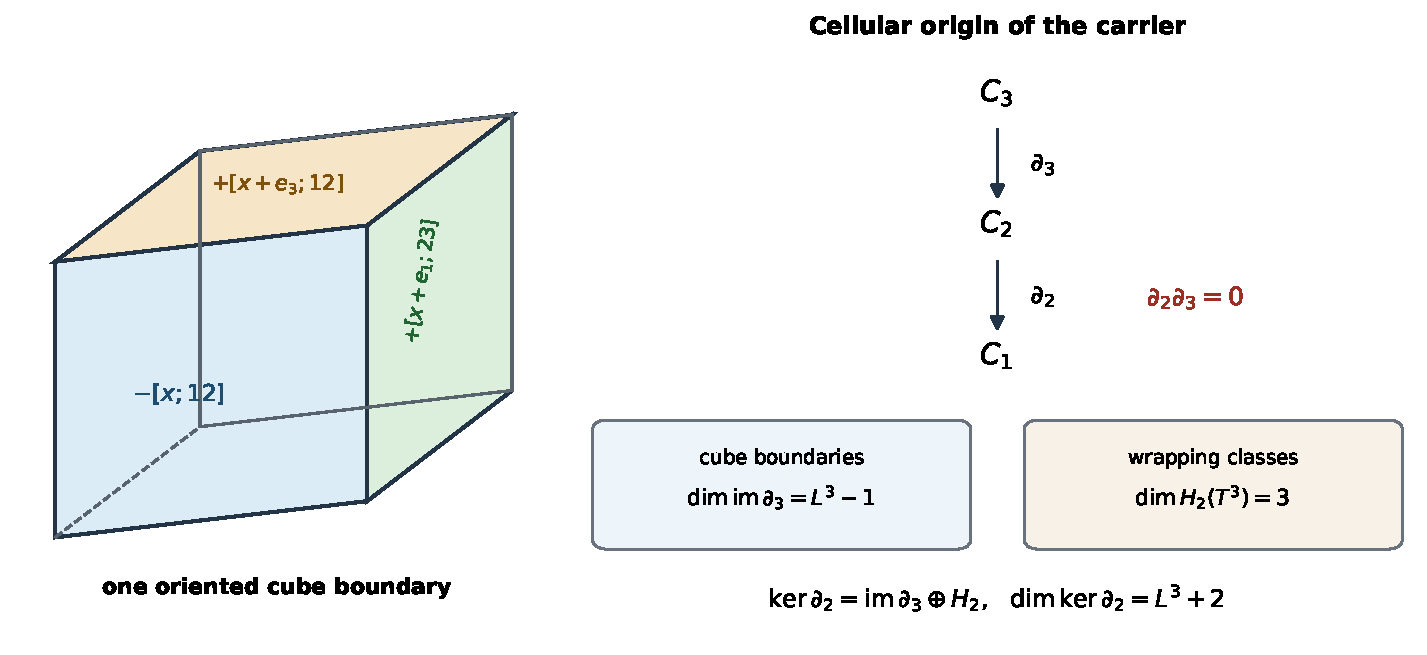
\includegraphics[width=0.97\textwidth]{figure_cellular_carrier.pdf}
\caption{The carrier is a cellular cycle space. The left panel shows three
visible terms in the outward-oriented boundary of one cube; the complete
six-face formula is given in Appendix~\ref{app:chain}. Cube boundaries span
$\operatorname{im}\partial_3$, while three noncontractible wrapping classes
complete $\ker\partial_2$ on the three-torus.}
\label{fig:cellular}
\end{figure}

The count is verified over $\mathbb{Z}$ rather than re-derived from the
formula: the complex is built from the boundary formulas of
Appendix~\ref{app:chain}; the exhibited cycles --- every elementary cube
boundary together with three wrapping sheets --- bound the kernel from below,
and rank over $\mathbb{F}_p$ bounds it from above, since rank can only drop
under reduction. The two bounds meet at $L=1,\dots,5$.
\chk{dim Z\_2 = L\^{}3 + 2 by rank, not by re-arranging the formula}
\chk{cube boundaries and three wrapping sheets SPAN Z\_2}

\begin{remark}
$L^3+2$ is the nullity of the down boundary Laplacian, not a Betti number; the
Betti contribution is the final $3$. The restriction $L\ge3$ belongs to the
twelve-neighbour Bloch adjacency, where $x+e$ and $x-e$ coincide at $L=2$. The
chain-level count has no such restriction and holds at $L=1,2$ as well.
\chk{the L\^{}3+2 count is chain-level, not the Bloch convention}
\end{remark}

The following sum rule joins Theorems~\ref{thm:fact} and~\ref{thm:carrier},
which are otherwise two unrelated statements: a $3\times3$ spectrum and an
$(L^3+2)$-dimensional space.

\begin{theorem}[Bloch--chain bridge]\label{thm:bridge}
On the periodic $L^3$ complex,
\[
  \sum_{k}\bigl(3-\operatorname{rank}B(k)\bigr)=L^3+2 ,
\]
the sum running over the $L^3$ allowed momenta, with nullity profile
$3$ at $\Gamma$ exactly once and $1$ at each of the other $L^3-1$ momenta.
\end{theorem}

\begin{proof}
$B(0)=0$ contributes $3$. For $k\neq0$ some $d_j\neq0$, and
Theorem~\ref{thm:fact} gives $\operatorname{rank}B(k)=2$, contributing $1$
each. Summing gives $3+(L^3-1)=L^3+2$.
\end{proof}
\chk{the Bloch and chain routes to the carrier agree}

\begin{remark}\label{rem:bridge}
Earlier editions of this paper read the agreement as a coincidence worth
checking --- ``the $3$ is the triple degeneracy of $B(0)=0$, not $b_2(T^3)$''.
That was wrong, and the correction is the better statement. Under the discrete
Fourier transform $\partial_2$ block-diagonalises and
$\ker\partial_2=\bigoplus_k\ker\partial_2(k)$; at $k\neq0$ the kernel block is
one-dimensional and is exactly $\operatorname{im}\partial_3(k)$, while
$\partial_3(0)=0$. So all of $\operatorname{im}\partial_3$ sits at nonzero
momenta and the quotient is supported entirely at $\Gamma$: the $\Gamma$ block
\emph{is} $H_2$, and the $3$ \emph{is} $b_2(T^3)$. The two routes do not agree
by accident; they are the same decomposition read in two bases.
\chk{the sheets average to harmonic representatives, and the Gamma block IS b\_2}
\end{remark}

The same block decomposition says exactly what a local seed costs at sharp
momentum.

\begin{proposition}[Fixed-momentum carrier and the locality tradeoff]\label{prop:locality}\label{prop:fixed-k-carrier}
Let $b_x=\partial_3[x;1,2,3]$ be the six-face boundary of the elementary cube
at $x$, and use the unitary discrete Fourier transform
$\hat b_L(k)=L^{-3/2}\sum_{x\in\Lambda_L}e^{-ik\cdot x}b_x$. For every allowed
$k\neq0$, $\hat b_L(k)$ has norm $\sqrt{q(k)}$ and, up to the Fourier phase
convention, is the vector $w(k)$ of Theorem~\ref{thm:fact}. Hence
$\varphi_L(k)=\hat b_L(k)/\sqrt{q(k)}$ is exactly the unique unit carrier
vector in that momentum fibre.

If $k_0=2\pi(r_1,r_2,r_3)/L_0\neq0$, then $k_0$ is an allowed momentum on
every nested volume $L=mL_0$, and the order-$u^2$ internal separation from
each of the two incidence branches is
\begin{equation}\label{eq:nested}
  t_Nu^2q(k_0),
\end{equation}
independent of $m$. More generally it is bounded below by $t_Nu^2q_*$ on any
set of allowed momenta with $q(k)\ge q_*>0$.

This exact sharp-momentum state is not local: it is the Fourier sum of all
cube boundaries. Conversely, for the normalised radius-one seed
$b_x/\sqrt6$,
\begin{equation}\label{eq:seedweight}
  \bigl|\langle\varphi_L(k),\,b_x/\sqrt6\rangle\bigr|
  =\sqrt{\frac{q(k)}{6L^3}},
\end{equation}
and $\hat b_L(0)=0$.
\end{proposition}

\begin{proof}
Fourier transforming the six terms of the cubical boundary gives, in the
$(12,13,23)$ face basis, $(d_3,-d_2,d_1)^T$, with conjugates if the opposite
Fourier sign is chosen. Its squared norm is $q(k)$ and
$\partial_2\partial_3=0$ puts it in $\ker B(k)\dg$; uniqueness for $k\neq0$
follows from Theorem~\ref{thm:fact}. The nested-volume statement is the
integer identity $k_0=2\pi(mr)/(mL_0)$, and \eqref{eq:nested} follows from
Corollary~\ref{cor:assembly}. Inverting the unitary Fourier transform gives
$b_x=L^{-3/2}\sum_k e^{ik\cdot x}\sqrt{q(k)}\,\varphi_L(k)$, which proves
\eqref{eq:seedweight}; the $k=0$ coefficient vanishes.
\end{proof}
\chk{the Fourier sum of cube boundaries IS the carrier, and a local seed costs L\^{}-3}

\begin{remark}[What the $L^{-2}$ collapse does and does not say]\label{rem:collapse}
The minimum of $q(k)$ over all nonzero finite-volume momenta is
$4\sin^2(\pi/L)$, so a contour isolating the single flat sheet from the other
two sheets uniformly over the entire Brillouin zone cannot follow from the
second-order symbol. This is an \emph{internal} sheet separation. It does not
erase the volume-uniform external electric-shell gap \eqref{eq:margin}, and it
does not affect the fixed-$k$ coefficient \eqref{eq:nested}. Neither fact by
itself controls the interacting Riesz projection or supplies transfer-matrix
overlap; those remain the substantive part of G18.
\end{remark}

\subsection{The wrapping sheets are cycles, not harmonic --- and their
harmonic representatives}

Theorem~\ref{thm:carrier} exhibits its three $H_2$ generators explicitly as
wrapping sheets $s_{(ij)}=\sum_{x:\,x_m=0}[x;i,j]$. These satisfy
$\partial_2 s=0$ exactly, so they are cycles and they span the quotient
$\ker\partial_2/\operatorname{im}\partial_3$. They are \emph{not} harmonic:
$\partial_3\dg s\neq0$, and
\begin{equation}
  \frac{\langle s,\;\partial_3\partial_3\dg\,s\rangle}{\|s\|^2}=2
  \qquad\text{exactly, for every }L\ge2 .
\end{equation}
\chk{FINDING: the wrapping sheets are cycles but NOT harmonic}

The distinction matters because $H_2$ is used in two senses: the quotient in
Theorem~\ref{thm:carrier}, which the sheets span, and the harmonic subspace
$\ker\partial_2\cap\ker\partial_3\dg$, which they do not lie in.

Harmonic representatives do exist, and they are one line away. Averaging a
sheet over its $L$ translates in the complementary direction,
\begin{equation}\label{eq:harmavg}
  h_{(ij)}=\frac1L\sum_{r=0}^{L-1}s_{(ij)}(r),\qquad
  \partial_2h_{(ij)}=0,\qquad \partial_3\dg h_{(ij)}=0,
\end{equation}
gives three harmonic chains spanning
$\ker\partial_2\cap\ker\partial_3\dg$, which is exactly three-dimensional; and
$s_{(ij)}-h_{(ij)}\in\operatorname{im}\partial_3$, so a sheet and its average
are the same homology class. The averaging is the $k=0$ Fourier projection,
and what it removes is precisely the non-harmonic part measured above ---
which is Remark~\ref{rem:bridge} again, in real space. Nothing about the
finding is withdrawn --- the generators Theorem~\ref{thm:carrier} exhibits are
still not harmonic --- but a real-space statement phrased for the harmonic
subspace now has representatives to point at, and
Proposition~\ref{prop:rigid} covers both, since $B\dg w=0$ holds on all of
$\ker\partial_2$.
\chk{the sheets average to harmonic representatives, and the Gamma block IS b\_2}

\section{Exact adjacent shared-link dynamics and global assembly}
\label{sec:second}

Two plaquettes sharing a link leave six nonshared fundamental links after the
external contractions. On the shared link the fusion channels depend on the
relative induced orientation,
\begin{equation}\label{eq:fusion}
  F\otimes\bar F=\mathbf{1}\oplus\mathrm{Adj},
  \qquad
  F\otimes F=\Lambda^2F\oplus\mathrm{Sym}^2F ,
\end{equation}
with dimensions and quadratic Casimirs
\begin{equation}\label{eq:table}
\begin{aligned}
  d_{\mathbf 1}&=1, & C_{\mathbf 1}&=0,\\
  d_{\mathrm{Adj}}&=N^2-1, & C_{\mathrm{Adj}}&=N,\\
  d_{\Lambda^2F}&=\tfrac{N(N-1)}2, & C_{\Lambda^2F}&=\tfrac{(N+1)(N-2)}N,\\
  d_{\mathrm{Sym}^2F}&=\tfrac{N(N+1)}2, & C_{\mathrm{Sym}^2F}&=\tfrac{(N-1)(N+2)}N.
\end{aligned}
\end{equation}

The six nonshared half-links contribute $3\CF$ and the fused link $C_\rho/2$,
against an external one-plaquette energy $2\CF$, so the resolvent denominator
is $\CF+C_\rho/2$ exactly.
\chk{each channel gap is C\_F + C\_R/2, and the weights sum to one}

\subsection{The channel weights are a theorem}

Earlier editions assigned the channel projector squared norm $d_\rho/N^2$ by
an isotropy hypothesis, and every statement in this section rests on that
assignment. It is not a hypothesis.

\begin{theorem}[Shared-link channel weights]\label{thm:weingarten}
In the normalised two-plaquette state, the weight of the shared-link channel
$\rho$ is exactly $d_\rho/N^2$, for both orientation families and every
$N\ge3$.
\end{theorem}

\begin{proof}
Two steps. First the six nonshared links collapse. Each plaquette contributes
a product of three independent Haar links, and a product of independent Haar
matrices is Haar, so the amplitude is
$\operatorname{Tr}(AU)\operatorname{Tr}(BU^{\pm1})$ with $A,B$ independent
Haar and $U$ the shared link. Integrating $A$ and $B$ contributes
$\delta/N$ each and leaves a pure degree-$(2,2)$ moment of $U$.

Second, two such moments settle both families. In the Weingarten calculus,
whose asymptotic origin is~\cite{Weingarten1978} and whose finite-$N$ closed
forms are~\cite{CollinsSniady2006}, the order-two values are
$\mathrm{Wg}(e)=1/(N^2-1)$ and
$\mathrm{Wg}((12))=-1/(N(N^2-1))$ --- the inverse of the $S_2$ Gram matrix
$\bigl(\begin{smallmatrix}N^2&N\\N&N^2\end{smallmatrix}\bigr)$ --- the index
sums give
\begin{equation}\label{eq:moments}
  \begin{aligned}
    M_{\mathrm{direct}}&=\sum_{ijkl}\bigl\langle|U_{ij}|^2|U_{kl}|^2\bigr\rangle=N^2,\\
    M_{\mathrm{cross}}&=\sum_{ijkl}\bigl\langle U_{ij}U_{kl}\bar U_{il}\bar U_{kj}\bigr\rangle=N .
  \end{aligned}
\end{equation}
The standard formula is often written for $U(N)$. A degree-$(2,2)$ integrand
is invariant under $U\mapsto zU$ for $z\in U(1)$, so integrating it over
$SU(N)$ and over $U(N)=\bigl(SU(N)\times U(1)\bigr)/\mathbb Z_N$ gives the
same number provided the $SU(N)$-invariants at this degree are exhausted by
the permutation contractions --- which holds exactly when the degree is below
the rank, so that no determinant (Levi-Civita) contraction is available. At
degree two this is the condition $N\ge3$, which is where the construction
already lives.
For the like family, $\operatorname{Tr}(AU)\operatorname{Tr}(BU)$ decomposes
into $\mathrm{Sym}^2\oplus\Lambda^2$ by symmetrising the two index pairs
jointly, and the two squared norms are
$(M_{\mathrm{direct}}\pm M_{\mathrm{cross}})/2$. Normalising,
\[
  n_{\mathrm{Sym}^2}=\frac{N+1}{2N}=\frac{d_{\mathrm{Sym}^2F}}{N^2},
  \qquad
  n_{\Lambda^2}=\frac{N-1}{2N}=\frac{d_{\Lambda^2F}}{N^2}.
\]
For the mixed family the singlet component of $U_{ij}\bar U_{lk}$ is
$\delta_{il}\delta_{jk}/N$, of squared norm $1$ against
$M_{\mathrm{direct}}=N^2$, so $n_{\mathbf 1}=1/N^2=d_{\mathbf 1}/N^2$ and
$n_{\mathrm{Adj}}=1-1/N^2=d_{\mathrm{Adj}}/N^2$.
\end{proof}
\chk{the shared-link weights are Weingarten, not an isotropy assumption}

\begin{remark}
The derivation imports nothing: the Weingarten pair is the inverse of the
$S_2$ Gram matrix and the index sums in \eqref{eq:moments} are explicit, so
the reader can check it without leaving this page. That the pair is not two
fitted constants is separately checked --- the identity-permutation value times
$N^2-1$ is $1$ identically in $N$, so the $SU(3)$ numbers are a specialisation
of a rank-generic formula. Together these make the \emph{local shared-link
coefficient} self-contained. By themselves they do not enumerate every
second-order process; that separate step is supplied by
Lemma~\ref{lem:exhaust}. Appendix~%
\ref{app:wg} records the index sums.
\chk{the Weingarten route is independent of the corpus}
\end{remark}

\begin{remark}[External corroboration]
The same numerator appears in the quantum-simulation literature from an
unrelated direction. Ciavarella, Burbano and Bauer~\cite{CBB2025} publish a
finite-rank plaquette matrix element
$|M_\rho|^2=\dim\rho/(\dim A\,\dim R)$; for two fundamental factors
$\dim A=\dim R=N$ and this is $d_\rho/N^2$ identically in $N$. That is
provenance for a chain already checked here, not a second derivation, and it
is not a second derivation. The exhaustion of the shared-link routes is
proved independently in Lemma~\ref{lem:exhaust}.
\chk{the published dimension-ratio matrix element is this registry's weight formula}
\end{remark}

\begin{remark}[A falsified zero backend]
The organized authority corpus contains an independent exact diagnostic at
$N=3$:
\[
 \mathrm{Wg}(e)=\frac18,\qquad
 \mathrm{Wg}((12))=-\frac1{24},\qquad
 \int_{SU(3)}|U_{11}|^4\,dU=\frac16\ne0.
\]
The related fourth moment $\int|U_{11}|^4\,dU=2/[N(N+1)]$ is $1/6$ at $N=3$
and in particular nonzero, which is what refuted a claimed Haar vanishing in
the balanced $(2,2)$ sector. It therefore falsifies the archived
stranded-flux rule that discards this sector. This is useful negative
evidence for retaining the contractions above; it is not a second derivation
of $t_N$.
\chk{the fourth moment integral |U\_11|\^{}4 = 1/6 at N = 3}
\end{remark}

\subsection{The off-diagonal process list is complete}
\label{sec:complete}

Write $X_q=\chi_q+\bar\chi_q$, so $V=\sum_q X_q$, and let
$Q_0=1-|0\rangle\langle0|$.

\begin{lemma}[Second-order process completeness]\label{lem:exhaust}\label{lem:process-complete}
For $N\ge3$, $L\ge3$, and distinct plaquettes $p,p'$, define
\begin{align}
  K_{2,-}&=P_-VQ_-(E_{F,N}-H_E)^{-1}Q_-VP_- ,\label{eq:K2}\\
  H^{\mathrm{exc}}_{2,-}&=K_{2,-}-E^{(2)}_{\mathrm{vac}}P_-,\qquad
  E^{(2)}_{\mathrm{vac}}=\langle0|VQ_0(0-H_E)^{-1}Q_0V|0\rangle .\label{eq:K2exc}
\end{align}
If $p$ and $p'$ share no link, then $\langle p',-|K_{2,-}|p,-\rangle=0$. If
they share the unique link $e$, every nonzero intermediate lies in exactly one
of $F\otimes\bar F=\mathbf1\oplus\mathrm{Adj}$,
$F\otimes F=\Lambda^2F\oplus\mathrm{Sym}^2F$ or the conjugate of the second
decomposition. Thus these four shared-link channels exhaust every
off-diagonal second-order process.

The conclusion is preserved by the stated link-Casimir budget cutoff, and more
generally by cutoffs that are functions only of the link Casimirs and
therefore act identically on all four orientation assignments. A general
projection inside the degenerate $2E_{F,N}$ eigenspace need not preserve the
non-adjacent cancellation.
\end{lemma}

\begin{proof}
Expand the external states and both insertions in oriented characters. A term
$\chi^\varepsilon_p\chi^\eta_q$, with $\varepsilon,\eta\in\{\pm1\}$ and
$\chi^{-1}=\bar\chi$, has linkwise centre charge
$\partial(\varepsilon p+\eta q)$ in $C_1(\Lambda_L;\mathbb Z_N)$. Since $H_E$
commutes with the independent link-centre actions, a common electric
intermediate between the $p$ and $p'$ sides requires
\begin{equation}\label{eq:centrematch}
  \partial(\varepsilon p+\eta q)=\partial(\varepsilon'p'+\eta'r)\pmod N
\end{equation}
for action plaquettes $q,r$ and signs $\varepsilon,\eta,\varepsilon',\eta'$.

We first record a small-support fact. A nonzero $2$-cycle over $\mathbb Z_N$
cannot be supported on at most four elementary plaquettes. Choose a supported
face $f$. Each of its four boundary links needs another supported face to
cancel its nonzero coefficient, while two distinct cubical faces share at most
one link. Four distinct additional faces would therefore be required.
\chk{the plaquette graph is 12-regular and two faces share at most one link}

Apply this fact to $z=\varepsilon p+\eta q-\varepsilon'p'-\eta'r$. Equation
\eqref{eq:centrematch} makes $z$ a $2$-cycle over $\mathbb Z_N$, so $z=0$
there. Because $p\neq p'$, the four occurrences must pair with opposite signs.
The only possibilities are
\begin{equation}\label{eq:sameface}
  q=p,\quad \eta=-\varepsilon,\quad r=p',\quad \eta'=-\varepsilon',
\end{equation}
or
\begin{equation}\label{eq:exchange}
  q=p',\quad r=p,\quad \eta=\varepsilon',\quad \eta'=\varepsilon .
\end{equation}
This also closes the determinant exceptions. For $SU(3)$ a coefficient $\pm3$
would require three occurrences of one face and leave a distinct fourth face
with coefficient $\pm1$; for $SU(4)$ a coefficient $\pm4$ would require all
four occurrences to be the same face. Both contradict $p\neq p'$.

The first alternative is absent from the charge-odd vector:
\[
  X_p|p,-\rangle=\frac{(\chi_p+\bar\chi_p)(\chi_p-\bar\chi_p)}{\sqrt2}|0\rangle
  =\frac{\chi_p^2-\bar\chi_p^2}{\sqrt2}|0\rangle ,
\]
so its same-face zero-$N$-ality component, including the vacuum, cancels. Only
the exchange alternative remains.

If $p,p'$ are link-disjoint, sharing a vertex being immaterial, linkwise
factorisation gives
$X_{p'}|p,-\rangle=\sqrt2\,|p,-\rangle|p',+\rangle$ and
$X_p|p',-\rangle=\sqrt2\,|p,+\rangle|p',-\rangle$. Both vectors have electric
energy $2E_{F,N}$, so the reduced resolvent is scalar on their span, while
their inner product is zero by charge orthogonality.

If $p,p'$ share $e$, the six nonshared links each carry one fundamental or
antifundamental factor and the shared link carries exactly two. The two
complete tensor-product decompositions above therefore give all common
intermediates. Their energies and gaps are
$E_\rho=3\CF+\tfrac12C_\rho$ and
$E_\rho-E_{F,N}=\CF+\tfrac12C_\rho>0$. Spectral resolution yields only their
four projectors. Vacuum subtraction is diagonal and leaves this cross matrix
element unchanged. The two-face term is connected, so the linked M\"obius
projection leaves it unchanged as well.
\end{proof}
\chk{connected first order vanishes by inclusion-exclusion, not by cancellation of numbers}

With Theorem~\ref{thm:weingarten} the resolvent weight is
\begin{equation}\label{eq:w}
  w_\rho=-\frac{d_\rho/N^2}{\CF+C_\rho/2},
\end{equation}
and summing within the two orientation families,
\begin{align}
  A_N&=w_{\mathbf 1}+w_{\mathrm{Adj}}=-\frac{2N^3}{(N^2-1)(2N^2-1)},\label{eq:AN}\\
  B_N&=w_{\Lambda^2}+w_{\mathrm{Sym}^2}=-\frac{4N(N^2-2)}{(N^2-1)(4N^2-9)}.\label{eq:BN}
\end{align}
\chk{the four channel weights follow from dimension and Casimir}
\chk{A\_N and B\_N are the channel sums, not transcriptions}

\subsection{The shared-link law}

\begin{theorem}[All-rank adjacent shared-link law]\label{thm:allrank}
Let $p\ne p'$ be oriented plaquettes sharing the single link $e$. For every
integer $N\ge3$, let $s=s(p,e)$, $s'=s(p',e)$, and let $\hat\Pi_\rho$ be the
charge-conjugation-closed electric projector onto the shared-link channel
$\rho$ (including the conjugate irrep on the conjugate like-channel
subspace). Define
\[
  \eta_\rho=
  \begin{cases}
    -1,&\rho\in\{\mathbf1,\mathrm{Adj}\},\\
    +1,&\rho\in\{\Lambda^2F,\mathrm{Sym}^2F\}.
  \end{cases}
\]
Then
\begin{equation}\label{eq:projroute}
  \hat\Pi_\rho X_{p'}|p,-\rangle=\eta_\rho ss'\,\hat\Pi_\rho X_p|p',-\rangle,
  \qquad
  \bigl\|\hat\Pi_\rho X_{p'}|p,-\rangle\bigr\|^2=\frac{d_\rho}{N^2},
\end{equation}
\begin{equation}\label{eq:channelme}
  \langle p',-|X_p\,\hat\Pi_\rho\,X_{p'}|p,-\rangle
  =\eta_\rho\,s(p',e)\,s(p,e)\,\frac{d_\rho}{N^2}.
\end{equation}
Consequently the linked order-$u^2$ contribution through all four channels is
\[
  \langle p',-|H_2|p,-\rangle
  =t_N\,s(p',e)s(p,e)
  =t_N(BB\dg)_{p'p},
\]
where $s(p,e)=\pm1$ is the cellular boundary incidence and
\[
  t_N=B_N-A_N=\frac{2N(N^2-4)}{(N^2-1)(2N^2-1)(4N^2-9)}>0 .
\]
\end{theorem}

\begin{proof}
Because distinct cubical faces share at most one link,
$(BB\dg)_{p'p}=ss'$. Expand
$|p;\varepsilon\rangle_{\mathrm{or}}:=\chi^\varepsilon_p|0\rangle$, with
$\chi^{+1}_p:=\chi_p$ and $\chi^{-1}_p:=\bar\chi_p$, so that
$|p,-\rangle=2^{-1/2}\sum_{\varepsilon=\pm1}\varepsilon\,
|p;\varepsilon\rangle_{\mathrm{or}}$.
On the shared link the two oriented factors are $\varepsilon s$ and
$\varepsilon's'$. A like channel requires $\varepsilon\varepsilon'=ss'$, while
a mixed channel requires $\varepsilon\varepsilon'=-ss'$. Thus the two
projected route vectors differ by exactly $\eta_\rho ss'$. Their two
charge-conjugate assignments are orthogonal for $N\ge3$; the two factors
$1/\sqrt2$ therefore sum to one channel weight, not twice one.
Theorem~\ref{thm:weingarten} gives the norm $d_\rho/N^2$, proving
\eqref{eq:projroute} and \eqref{eq:channelme}.

On this channel,
$(E_{F,N}-H_E)^{-1}\hat\Pi_\rho=-\hat\Pi_\rho/(\CF+C_\rho/2)$. Its
contribution is therefore $\eta_\rho ss'w_\rho$. Summing gives
$ss'\bigl(w_{\Lambda^2F}+w_{\mathrm{Sym}^2F}-w_{\mathbf1}-w_{\mathrm{Adj}}\bigr)
 =ss'(B_N-A_N)$. Substitution of \eqref{eq:AN}--\eqref{eq:BN} gives the
displayed rational function. Every denominator factor and $N^2-4$ is positive
for $N\ge3$.
\end{proof}
\chk{t\_N = B\_N - A\_N}\chk{t\_N > 0 for N >= 3}

The opening geometric ingredient of the proof is no longer prose: the
verifier enumerates every distinct face pair of the periodic complex at
$L=3$ and $L=4$ and confirms that no pair meets in more than one link. Two
faces sharing a link span at most two sites per axis, so these windows
already exhibit every local configuration and larger $L$ adds translates
only.

\begin{corollary}[Global torus assembly]\label{cor:assembly}
On the trivial-flux charge-odd electric shell of Theorem~\ref{thm:window},
translation and cubic symmetry make the remaining diagonal contribution a
scalar, and
\[
  H^{(N)}_{\mathrm{eff},-}(k,u)
  =E_{\mathrm{flat},N}(u)I+t_Nu^2B(k)B(k)\dg+O(u^3).
\]
Consequently the three bands through second order are
$E_{\mathrm{flat},N}(u)$ and
$E_{\mathrm{flat},N}(u)+t_Nu^2q(k)$ twice, and the flat carrier is
$\ker\partial_2$, of dimension $L^3+2$.
\end{corollary}

\begin{proof}
The centre-charge argument of Lemma~\ref{lem:exhaust}, now with only three
plaquette occurrences, gives
$\langle p',-|P_-VP_-|p,-\rangle=0$ for $p\neq p'$. A possible $SU(3)$
determinant balance would require all three occurrences to be the same face
and is therefore excluded off diagonal. Translation and cubic symmetry make
the remaining first-order diagonal a scalar, including any $SU(3)$ same-face
determinant contribution, and it is absorbed into $E_{\mathrm{flat},N}(u)$.

At second order Lemma~\ref{lem:exhaust} and Theorem~\ref{thm:allrank} assemble
every off-diagonal entry. Translations act transitively on faces of a fixed
orientation and the cubic group permutes the orientations, so the invariant
second-order diagonal is also a multiple of the identity. Thus the adjacency
part is $t_N(BB\dg-4I)$; absorb $-4t_N$ into the scalar and apply
Theorem~\ref{thm:fact}.
\end{proof}

The status change deserves one sober sentence rather than celebration. What
earlier editions carried as two prose premises is now proved relative to the
standard degenerate perturbation framework of \eqref{eq:heff}, the classical
Casimir arithmetic of Theorem~\ref{thm:window}, and the centre-charge
classification of Lemma~\ref{lem:exhaust}. The finite-volume $L=3,4,5$
enumerations in the verifier are regressions on those proofs, not substitutes
for them. The charge-even identification of Section~\ref{sec:even} remains a
hypothesis, and nothing about convergence, higher orders, or the continuum has
changed.

Two consequences,
\begin{equation}\label{eq:tsmall}
  t_3=\frac{5}{612},\qquad
  t_N=\frac1{4N^3}-\frac1{16N^5}-\frac{77}{64N^7}-\frac{1021}{256N^9}+\cdots
\end{equation}
\chk{t\_2 = 0 and t\_3 = 5/612}\chk{large-N expansion of t\_N through 1/N\^{}9}

The expansion is governed by a closed form. Writing the planar-normalised
coefficient as $4N^3t_N$,
\begin{equation}\label{eq:planar}
  1-4N^3t_N=\frac{2N^4+31N^2-9}{(N^2-1)(2N^2-1)(4N^2-9)},
\end{equation}
an identity of rational functions, and the right side is positive and the
left strictly decreasing for every real $N\ge2$: substituting $N=M+2$ makes
every numerator coefficient of both the remainder and the derivative
nonnegative, so $4N^3t_N$ increases monotonically to $1$. At fixed canonical
coordinate $u$ the conditional bandwidth of Corollary~\ref{cor:assembly} is
$12t_Nu^2$, so the entire dispersive content of the projected sector
switches off at exactly the rate $N^{-3}$, with computable subleading
coefficient $-1/(4N^2)$: conditional on the assembly, the carrier's exact
degeneracy is approached by the \emph{whole} sector in the planar limit.
This is consistent with the general suppression of glueball mixing at large
$N$, but no 't~Hooft-coupling identification is made here: the statement is
about the coefficient in the canonical coordinate, and it is exact.
\chk{deficit identity 1/4 - N\^{}3 t\_N}
\chk{N\^{}3 t\_N increases monotonically to 1/4}

\subsection{The vacuum-mediated route}

Lemma~\ref{lem:exhaust} is specific to the charge-odd shell. The
corresponding assertion is false in general: the charge-even sector admits a
vacuum-mediated route. Its cancellation in the odd sector is the
charge-conjugation selection rule below, and omitting it is a recorded error,
not a hypothetical one.

\begin{proposition}[Vacuum-mediated route]\label{prop:vacuum}
The reduced-resolvent route
\[
 \frac{\langle p'|V|0\rangle\langle 0|V|p\rangle}{E_{F,N}-E_0}
 =\frac{\langle p'|V|0\rangle\langle 0|V|p\rangle}{E_{F,N}}
\]
is available for any
pair of plaquettes, sharing a link or not. It vanishes identically in the
charge-odd sector, because $V$ is charge-even and $|0\rangle$ is charge-even,
so $\langle0|V|p,-\rangle=0$. Consequently the charge-odd hopping
$t_N=B_N-A_N$ carries no such term, while the charge-even shared-link element
acquires $1/\CF$: the normalised charge-even matrix-element product is $2$
and $E_{F,N}=2\CF$.
\[
  \ell_N=A_N+B_N+\frac1{\CF}
  =-\frac{2N(3N^2-5)}{(N^2-1)(2N^2-1)(4N^2-9)} .
\]
\end{proposition}
\chk{ell\_N = A\_N + B\_N + 1/C\_F, the vacuum-mediated route at every rank}

\begin{remark}
At $N=3$, $A_3+B_3=-481/612$ and $1/\CF=3/4$, giving $\ell_3=-11/306$. The
first of these is exactly the value once published for the charge-even hopping
and later superseded; the correction is precisely the omitted route. Stating
the selection rule turns a one-rank erratum into an all-rank formula.

In the charge-odd shell, Lemma~\ref{lem:exhaust} and this proposition dispose
of non-adjacent pairs: the exchange vectors are orthogonal and the vacuum
route vanishes. In the charge-even sector, however, this proposition does not
dispose of the non-adjacent vacuum route. Taken over all pairs it would be a
rank-one operator supported at $k=0$, not the twelve-neighbour adjacency
multiplied by $\ell_N$. The check above establishes the all-rank shared-link
value $\ell_N$; the reorganisation or cancellation of the charge-even
all-pairs term remains a separate requirement.
\end{remark}

\subsection{Finite-volume width}

Let $q_{\max}(L)$ be the largest sampled $q$ on the periodic $L^3$ grid. Then
\begin{equation}\label{eq:qmax}
  q_{\max}(L)=
  \begin{cases}
    12, & L\text{ even},\\[2pt]
    12\cos^2\!\bigl(\pi/2L\bigr), & L\text{ odd},
  \end{cases}
\end{equation}
because only at even $L$ does some $k_j$ reach $\pi$ exactly. The width of the
full retained charge-odd manifold is $W^{(-)}_{N,L}=q_{\max}(L)\,t_Nu^2+O(u^3)$,
so for even $L$, and coefficientwise as $L\to\infty$ at fixed perturbative
order, $[u^2]W^{(-)}=12t_N\sim3/N^3$.
This concerns the stiffness of the dispersive doublet, not motion of the
lowest branch, which is flat at this order.
\chk{the zone maximum of q is 12 only at even L}

The smallest nonzero incidence eigenvalue is $q_{\min}=4\sin^2(\pi/L)$,
attained by one unit of momentum in a single direction.
\chk{q\_min on the L-torus grid is 4 sin\^{}2(pi/L)}

\begin{figure}[t]
\centering
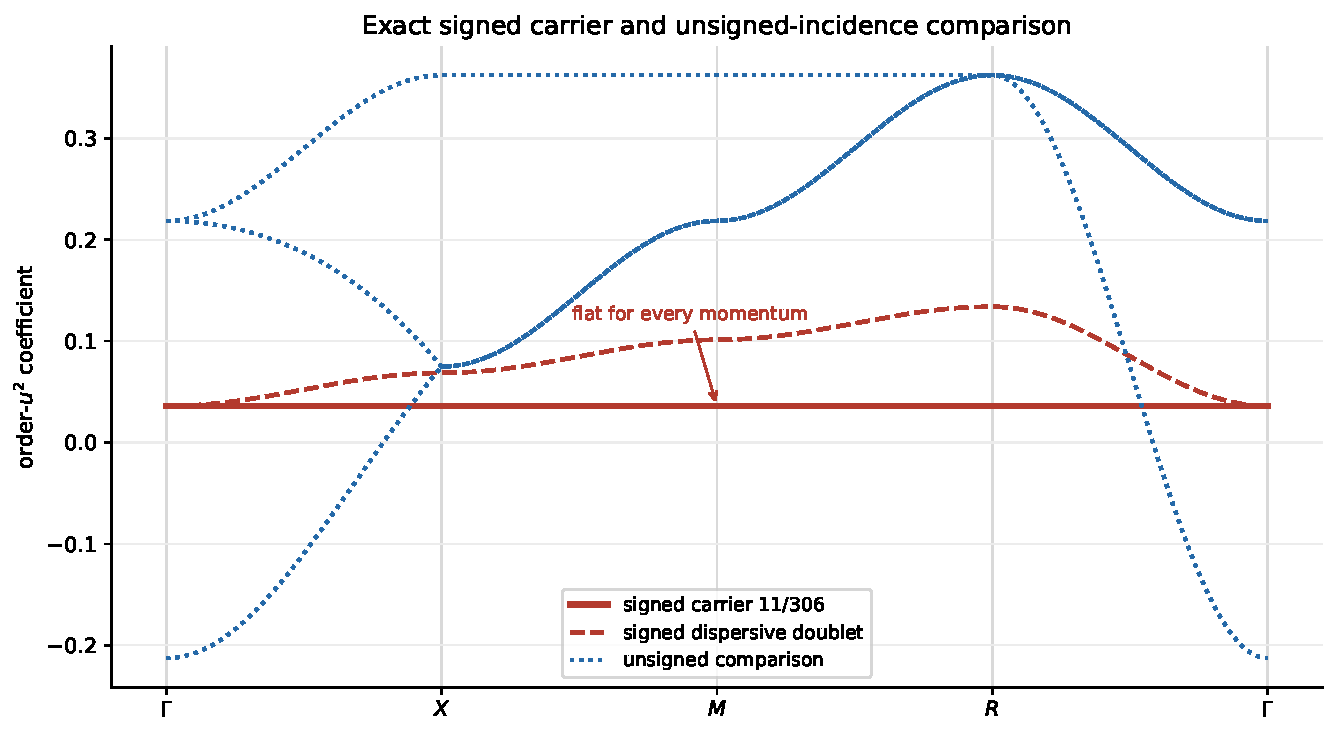
\includegraphics[width=0.94\textwidth]{figure_second_order_bands.pdf}
\caption{Order-$u^2$ coefficients along
$\Gamma$--$X$--$M$--$R$--$\Gamma$. The red carrier and dispersive doublet
are the signed incidence result; their conditional global assembly is
Corollary~\ref{cor:assembly}. The blue curves are the exact unsigned-incidence
comparison spectrum. Reading the blue curves as physical charge-even bands
requires the separate symbol hypothesis of Section~\ref{sec:even}.}
\label{fig:secondorder}
\end{figure}

\subsection{The orientation signs are essential}

Removing the orientation signs --- from the entries of \eqref{eq:B} and from
the phases, so each $e^{ik}-1$ becomes $e^{ik}+1$ --- gives an unsigned
incidence $\mathcal N(k)$. Define its comparison adjacency by
$A_+(k):=\mathcal N(k)\mathcal N(k)\dg-4I$.
Its adjacency spectra at $\Gamma$ and $R$ are $\{12,0,0\}$ and $\{-4,-4,-4\}$,
which share no eigenvalue, so no level can be momentum independent. The flat
branch is therefore not a generic consequence of three face orbitals or cubic
symmetry.

Section~\ref{sec:even} computes the unsigned comparison spectrum in closed
form. The signed span is $8-(-4)=12$, giving the charge-odd second-order width
$12t_3=5/51$ at $N=3$. The unsigned continuous-zone span is
$12-(-4)=16$. Interpreting $16|\ell_3|=88/153$ as a charge-even bandwidth is
conditional on deriving the complete linked charge-even symbol; on a finite
torus the value $-4$ is sampled only when $L$ is even.
\chk{the two band spans ARE the two incidence spectra}

\section{The second-order coefficient on a two-cube space}
\label{sec:twocube}

Everything above derives $t_N$ from a resolvent ledger indexed by the fusion
channel of one shared link. That ledger is representation theory carried out on
a single plaquette pair; it has never been tested against an operator
calculation on a space large enough for two cubes to interact. This section
reports such a test and, more importantly, states what it settles.

The construction is the open face-sharing $(3,2,2)$ prism with its eleven
oriented plaquettes, in the exact-Casimir $\mathcal B=6$ $SU(3)$ truncation, of
basis dimension $1{,}590{,}462$. The delivery reports that it reaches the
relevant sector through $794$ paths and $398$ reachable states; it does not
assemble a $1{,}590{,}462$-dimensional magnetic matrix. Its complete
charge-odd one-plaquette shell at
$E_*=8/3$ has dimension eleven --- a census result and not the plaquette count.
The full $E_*$ eigenspace has dimension $22$, split $11_{C=+}\oplus11_{C=-}$ by
tensor-derived charge conjugation, and the delivery removes all $22$ from the
pseudoinverse; because the eleven columns exhaust the odd half, that agrees
with the $Q=1_--P_-$ prescription of \eqref{eq:heff}. Writing $K_{LR}$ for the raw second-order
operator and $K_L,K_R,K_F$ for the left-cube, right-cube and shared-face
operators in their own coordinates, the connected operator is defined by the
literal M\"obius fold
\begin{equation}\label{eq:mobius}
  K_{\mathrm{conn}}=K_{LR}-J_LK_LJ_L\dg-J_RK_RJ_R\dg+J_FK_FJ_F\dg ,
\end{equation}
and the same fold applied to the geometry gives $G_{\mathrm{conn}}$. The fold
is literal in the sense that no eigenvalue or fitted scalar is subtracted: each
source operator is folded in its own coordinates and lifted. The delivery
corroborates that internally by applying the same weights history by history
over its $1{,}984$ ordered two-step histories, of which $1{,}192$ cancel at
weight zero, and the two routes agree to $4.9\times10^{-15}$.

First order settles itself. On the shell $PVP=I_{11}$, so the first-order term
is nonzero but scalar: it shifts all eleven branches equally and creates no
branch ambiguity. Its connected fold then vanishes \emph{identically}, and by
counting rather than by cancellation --- each of the eleven faces is covered
exactly once by $\{L,R\}$ once the shared face is restored by $F$, so every
M\"obius weight in \eqref{eq:mobius} applied to the identity is $1-1=0$.
Second order is therefore the leading connected term and not a correction to a
first-order one.
\chk{connected first order vanishes by inclusion-exclusion, not by cancellation of numbers}

At second order the result is
\begin{equation}\label{eq:kconn}
  K^{(2)}_{\mathrm{conn}}=\frac{5}{612}\,G_{\mathrm{conn}}+D ,
\end{equation}
with $D$ diagonal and delivered. The geometry alone fixes the \emph{splitting}
inside each block and nothing else: $G_{\mathrm{conn}}$ turns out to be four
disjoint $2\times2$ blocks plus three isolated directions
(Appendix~\ref{app:twocube}), so each pair splits by $2\times5/612=5/306$ about
its own diagonal entry. Given $D$, which Appendix~\ref{app:twocube} prints,
  the spectrum is then closed form: $0$ once, $-\tfrac{15}4$ twice,
  $-\tfrac{34}9$ four times, and $-\tfrac{129}{34}$ four times ---
exact arithmetic on entries that are themselves reconstructions, a boundary
made precise below.
The delivery reports the coefficient recovered target-blind --- supplied to no
builder, graph fit, branching rule or validator --- and reports that the payload
hashes were produced before the recorded comparison, a chronology it itself
calls record-backed and only partly auditable; the value is byte-present in the
nested $\mathcal B=4$ package that the $\mathcal B=6$ build seals as an authority object, so the
defensible statement is dependency-path nonuse and not corpus-wide absence.
This paper re-thresholds those delivered gates rather
than re-running the build, including a deliberately wrong-sign control that the
held-out scaling rejects: on a $66$-dimensional held-out word space the correct
second-order residual falls with log-log slope $2.90$ while the sign-reversed
control falls with slope $2.00$, a minimum error ratio of $325$. What all this
establishes is runtime nonuse of the comparator on the delivered dependency
path, which is not a preregistration. The finite-$u$ validations are
asymmetric: the $\mathcal B=4$ delivery includes a held-out diagonalisation of
the full $4{,}180$-dimensional charge-odd space with an $O(u^3)$ residual,
whereas the $\mathcal B=6$ check is restricted to the $66$-dimensional
$P+Q_1$ star.
\chk{the connected two-cube geometry has exactly four cross-cell pairs, each -1}
\chk{the B=6 connected kernel is (5/612) G\_conn + diag, with the certified spectrum}
\chk{the certificate's own gates pass, target-blind, with the wrong-sign control rejected}

Resolving \eqref{eq:kconn} by the irreducible representation the shared link
actually carries in the ranked intermediate state gives six coefficients rather
than four, because a link distinguishes $\rho$ from $\bar\rho$:
\begin{equation}\label{eq:census}
\begin{array}{c|cccccc}
 \rho & \mathbf1 & \mathbf3 & \bar{\mathbf3} & \mathbf6 & \bar{\mathbf6} & \mathbf8\\
 \hline
 c_\rho & \tfrac1{12} & -\tfrac1{12} & -\tfrac1{12}
        & -\tfrac19 & -\tfrac19 & \tfrac{16}{51}
\end{array}
\end{equation}
\chk{the B=6 six-channel census sums to the registry's own t\_3 = 5/612}

That these six sum to $5/612$ is weak evidence: six rationals reach one target
in many ways, and a fitted set would pass it. The statement worth making is
stronger, and it is what makes this more than a coincidence of one sum. First,
though, the boundary.

The six coefficients of \eqref{eq:census} are not symbolic: the delivery
stores them as rational reconstructions of pinned finite-precision
Clebsch--Gordan contractions, with a maximum reconstruction residual of
$2.2\times10^{-15}$ per channel --- $2.1\times10^{-14}$ across the delivery's
reconstructed matrices as a whole --- and its own certificate declaring
\texttt{symbolic\_exact\_local\_amplitudes: false}. What follows is therefore
reported, conditional on those six numbers, and not a symbolic identity in the
sense of Theorem~\ref{thm:weingarten}.

\begin{reported}[The census is the Weingarten ledger]\label{rep:census}
At $N=3$ the six reconstructed link-irrep coefficients of \eqref{eq:census}
are the four fusion-channel weights \eqref{eq:w} individually:
\[
  c_{\mathbf 1}=-w_{\mathbf 1},\qquad
  c_{\mathbf 8}=-w_{\mathrm{Adj}},
\]
\[
  c_{\mathbf 3}=c_{\bar{\mathbf 3}}=\tfrac12 w_{\Lambda^2F},\qquad
  c_{\mathbf 6}=c_{\bar{\mathbf 6}}=\tfrac12 w_{\mathrm{Sym}^2F}.
\]
\end{reported}

\noindent Substituting \eqref{eq:table} into \eqref{eq:w} at $N=3$ gives
$w_{\mathbf 1}=-1/12$, $w_{\mathrm{Adj}}=-16/51$, $w_{\Lambda^2F}=-1/6$ and
$w_{\mathrm{Sym}^2F}=-2/9$; comparison with \eqref{eq:census} is then
arithmetic. Six reconstructed rationals landing on four predicted ones, with
the two coincidences the correspondence requires, is a strong consistency
statement and not a proof that the underlying contraction is exact.
\chk{the B=6 six-channel census IS the Weingarten four-channel ledger, channel by channel}

One further feature of the census is worth separating out, because it is the
paper's central architecture measured rather than assumed. The six
link-resolved matrices are not merely six numbers that sum correctly: each is
\emph{separately} proportional to the same incidence Gram. The eleven oriented
plaquettes of the prism have exactly $56$ ordered adjacent pairs, each sharing
one link with signed overlap $\pm1$; the delivery reports a constant
channel-to-geometry ratio on all $56$ of them, for every one of the six
channels, with worst residual $2.2\times10^{-15}$. Colour dynamics fixes a
number per channel and the cellular boundary operator fixes the matrix; if the
two mixed, the ratio would be constant for the total and not for the parts.
\chk{every shared-link channel is separately proportional to the geometry, on all 56 pairs}

The correspondence is scoped to what the Casimir closure exhausts: adjacent,
one-action, shared-link intermediates at order $u^2$. Same-face diagonal
routes, on-site terms and higher-action intermediates lie outside it --- the
$\mathcal B=6$ scalar below is exactly a place where one of them is missing --- and so
does any untruncated-Hilbert-space statement.

It is scoped in one further way, which matters more. The two-cube build draws
its local Wilson amplitudes from the same hash-pinned upstream
Clebsch--Gordan archive as the single-cube reconstructions of the next
subsection, and the squared amplitudes that archive produces are the published
$d_\rho/N^2$~\cite{CBB2025} --- the numerator of \eqref{eq:w}. The census
therefore does not confirm the weights from an independent source: it tests the
\emph{assembly} that carries them, which is the reachable-channel list, the
resolvent denominators, the operator-level fold, the even split between
conjugates, and the geometry that survives each channel separately. That is the
statement worth making, and it is a different statement from confirmation.

Two features of the correspondence carry the content. The mixed family enters
negated because $t_N=B_N-A_N$, which is the same relative sign the incidence
orientation carries. And each like-family \emph{fusion} weight is split evenly
between the irrep and its conjugate --- the two orientations of the shared link
weighted equally --- which the delivery resolves on the two-cube space rather
than assuming. It is not measured \emph{here}: what this repository checks is
the identity the six delivered numbers satisfy.

\begin{conjecture}[All-rank even split]\label{conj:split}
For every $N\ge3$ each like-family fusion weight splits evenly between an
irrep and its conjugate in the link-resolved census.
\end{conjecture}

\noindent This is a conjecture and nothing here promotes it. Falsifying it
means a link-resolved census at some $N\ge4$ in a truncation that still
retains every adjacent shared-link channel; at $N=4$ the endpoint budgets make
that $\mathcal B\ge33/4$, and no such construction has been run.

\subsection{One truncation, two constructions}

The two-cube space also isolates why a cutoff can reverse the sign of $t_3$.
An adjacent shared-link channel $\rho$ is reachable only if the endpoint
Casimir budget $C_2(\rho)+2C_2(\mathbf 3)$ fits inside the truncation, meaning
$C_2(\rho)+2C_2(\mathbf 3)\le\mathcal B$: the sextet needs exactly $6$ and the
adjoint $17/3$, so both survive $\mathcal B=6$ and neither survives
$\mathcal B=4$.

The weak inequality is not a convenience. Both retentions this section uses
are decided by an equality: $\Lambda^2F=\bar{\mathbf3}$ has budget exactly $4$
and so sits exactly on the $\mathcal B=4$ cutoff, and the sextet sits exactly
on the $\mathcal B=6$ one. Under a strict rule $\mathcal B=4$ would reach
$\{\mathbf 1\}$ alone and $\mathcal B=6$ would lose the sextet, contradicting
both delivered censuses --- so the deliveries are what fix the convention,
which is also why the budget arithmetic is not an independent confirmation of
either census.
\chk{B=6 retains every adjacent shared-link channel; B=4 provably cannot}
\chk{the retention rule is C2(rho) + 2 C2(3) <= B, and both retentions it decides are equalities}

\begin{corollary}[What a link cutoff drops]\label{cor:cutoff}
Retaining only the singlet and $\Lambda^2F$ routes projects the second-order
hopping to
\[
  w_{\Lambda^2F}-w_{\mathbf 1}=-\tfrac1{12},
\]
opposite in sign to $t_3$ and $10.2$ times larger in magnitude. What is
dropped is
\[
  w_{\mathrm{Sym}^2F}-w_{\mathrm{Adj}}=\tfrac{14}{153},
\]
and $-\tfrac1{12}+\tfrac{14}{153}=\tfrac5{612}=t_3$. This is arithmetic on
\eqref{eq:w} alone.
\end{corollary}

\noindent The published $p+q\le1$ link cutoff retains exactly those two
routes --- a per-link restriction, where $\mathcal B=4$ is a total endpoint
budget, so the two schemes agree on the retained channels at this order and are
not the same rule --- so $-1/12$ is its projected adjacent hopping and
$14/153$ is the adjacent-hopping correction that completes it --- not
$5/612$, which would double-count what it already carries. On the two-cube
space the first of those two numbers is delivered rather than inferred: a
separately sealed $\mathcal B=4$ run on the identical geometry gives
$K^{(2),\,\mathcal B=4}_{\mathrm{conn}}=-\tfrac1{12}G_{\mathrm{conn}}+D_{\mathcal B=4}$
outright, and the Casimir budgets of the previous paragraph say without
reference to any census that $\mathcal B=4$ can reach only
$\{\mathbf1,\mathbf3,\bar{\mathbf3}\}$. Conditional on \eqref{eq:census}, the
same split of the census reproduces it,
$c_{\mathbf 1}+c_{\mathbf 3}+c_{\bar{\mathbf 3}}=-1/12$, and gives the omitted
half as $c_{\mathbf 6}+c_{\bar{\mathbf 6}}+c_{\mathbf 8}=14/153$.
\chk{the B=6 six-channel census IS the Weingarten four-channel ledger, channel by channel}
\chk{FINDING: the T1 link cutoff reverses the sign of t\_3, and 14/153 is what it omits}

\begin{remark}
Two single-cube reconstructions bracket the same statement. A full $\mathcal B=4$ open
cube assembled from the pinned \texttt{ymcirc} $d=3$, $\mathcal B=4$ plaquette data
~\cite{Balaji2026,ymcirc2026} reproduces $-1/12$ and the truncated shell ordering to
$4.3\times10^{-11}$; a $\mathcal B=6$ cube reproduces $+5/612$ and the inverse ordering
to $8.4\times10^{-15}$. Both locate the missing weight at the same $14/153$.

Neither is an independent replication. Both read tabulated plaquette matrix
elements of the same lineage --- and the two-cube build draws its
Clebsch--Gordan amplitudes from the same hash-pinned \texttt{pyclebsch} archive
as the $\mathcal B=6$ cube, so that agreement is a cross-check of assembly and not of
the amplitudes. The published closed form~\cite{CBB2025} is
$d_\rho/N^2$ --- the very numerator of \eqref{eq:w}. This is a cross-check of
assembly, not a third confirmation of $t_3$; the exact rational identity is
Corollary~\ref{cor:cutoff}, which needs no tolerance. The $p+q\le1$
nomenclature and the finite-rank matrix element are both from~\cite{CBB2025},
and single-cube $SU(N)$ diagonalisation in this style goes back
to~\cite{CM2003}.

The correction to the adjacent-hopping coefficient of a published $T_1$
Hamiltonian is therefore $14/153$ and not $5/612$, which would double-count
the two routes $T_1$ already carries. One coincidence of value is worth naming:
$-1/12$ is also the singlet weight $w_{\mathbf 1}$, and the cutoff value is a
\emph{difference} of two weights, not a weight.
\chk{FINDING: a full T1 = B = 4 cube Hamiltonian reproduces -1/12 and the reversed shell}
\chk{FINDING: the B = 6 cube flips the sign back to +5/612, closing the decisive test}
\end{remark}

The $\mathcal B=6$ cube is channel-complete for the hopping and \emph{not} for the
scalar: its scalar is $39/68$ against the bridge's $11/34$, differing by
exactly $1/4$, the local same-face sextet route, which first enters at cutoff
$20/3$ --- integer label $\mathcal B=7$, so any cutoff above $20/3$ already carries it.
\chk{the B = 6 scalar misses the bridge's by exactly the same-face sextet route}

That is a prediction with a cheap test, and the test was executed. A six-face
$\mathcal B=7$ reachable-state probe returns $\alpha_{\mathcal B=7}=11/34$ and
$t_{\mathcal B=7}=5/612$ with scalar-plus-Gram residual $1.1\times10^{-15}$, so
raising the cutoff past the same-face threshold lowers all three absolute
coefficients by exactly $1/4$ and leaves the relative shell
$\{0,\,5/153,\,5/102\}$ untouched --- the scalar moves, the hopping does not.
That probe's artifact did not travel, so it is reported here and not checked.

\subsection{What the cutoff moves, and where}

The connected diagonal $D$ is eleven numbers in both deliveries and is treated
as a remainder in both. It is not eleven numbers. The open prism has a symmetry
group --- the cell exchange $x\mapsto2-x$, the two transverse reflections and
the $y\leftrightarrow z$ swap, of order $16$ --- and $D$ is constant on its
orbits, which are $8+2+1$: the eight side faces, the two end caps, the shared
face.

\begin{proposition}[Where the truncation lives]\label{prop:orbit}
The eight-element orbit is exactly the support of the four cross-cell pairs,
and it is the only orbit whose diagonal value differs between the two
truncations: the end caps carry $-15/4$ and the shared face $0$ at both
$\mathcal B=4$ and $\mathcal B=6$, while the side value moves from $-7/4$ to
$-2317/612$. Together with
the four cross-cell blocks carrying the whole off-diagonal change, the entire
$\mathcal B=4\to\mathcal B=6$ difference is confined to the faces that carry connected transport.
\end{proposition}
\chk{the connected diagonal is orbit-constant, and only the transporting orbit moves}

This also says what the nonuniform $D$ is. Where the faces of a complex form a
\emph{single} orbit --- the closed cube of the next subsection, or the periodic
torus of Corollary~\ref{cor:assembly} --- orbit-constancy forces the diagonal to
be scalar, and the operator is exactly $\alpha I+tG$. The prism has three
orbits because it has a boundary. $D$ is the open boundary showing up in the
diagonal, not a failure of the incidence form.

\subsection{The one-cube shell, and why its flat level cannot move}

Those two single-cube reconstructions are usually read as numerical
cross-checks. They are more than that, because the object they diagonalise is
the same chain complex. The six faces of a cube are a closed surface, so in the
outward orientation $\ker\partial_2$ is one-dimensional and spanned by the sum
of all six --- the fundamental class, $b_2(S^2)=1$. That is
Theorem~\ref{thm:carrier} on a complex with no three-cells, where the $L^3-1$
boundaries are absent and only the class survives.

\begin{proposition}[One-cube shell]\label{prop:cube}
On the closed cube surface $G=\partial_2^{\mathsf T}\partial_2$ commutes with
all $24$ proper rotations. The combinations $b_{+i}-b_{-i}$ carry the defining
vector representation and the combinations $b_{+i}+b_{-i}$ the permutation
representation of the three unordered axes, so with the charge-odd inversion
$Pb_{+i}=-b_{-i}$ the shell is
\[
  A_1^{--}\oplus T_1^{+-}\oplus E^{--},
\]
with $G$-eigenvalues $0$, $4$, $6$ and multiplicities $1$, $3$, $2$.
Consequently $\alpha I+tG$ has levels $\alpha$, $\alpha+4t$, $\alpha+6t$.
\end{proposition}

\begin{proof}
The rotations permute the six outward faces, and $G$ is built from the boundary
map, so it commutes with the permutation action. On the antisymmetric
combinations that action is the defining representation by inspection --- $b_{+i}-b_{-i}$
transforms as $e_i$ --- and on the symmetric combinations it is the
permutation representation of $\{\pm e_i\}$, which is $A_1\oplus E$. Under
$Pb_{+i}=-b_{-i}$ the antisymmetric sector is parity even and the symmetric one
parity odd. In these sectors $G$ is $4I$ and $4I-2(J-I)$ respectively, of
spectra $\{4,4,4\}$ and $\{0,6,6\}$; since the three isotypic components have
distinct dimensions the eigenvalues attach to them uniquely.
\end{proof}
\chk{the one-cube shell is A1 + T1 + E, and its flat level is the S\^{}2 fundamental class}

Three things follow. The cubic labels are derived here rather than assigned:
both deliveries assert them and neither builds the symmetry matrices. The
$A_1^{--}$ level is Proposition~\ref{prop:rigid}'s mechanism on a second
complex --- $Gw=0$ there, so that level sits at $\alpha$ for every $t$, and no truncation, no
channel and no coefficient in dispute anywhere in this paper can move it. And
the reversal the two runs report is therefore a statement about the sign of one
number rather than about the shell as a whole: at $\mathcal B=6$ the levels are
$\{39/68,\,371/612,\,127/204\}$ and at $\mathcal B=4$ $\{37/12,\,11/4,\,31/12\}$, in
the opposite order, with $A_1^{--}$ in each case sitting exactly at the scalar.
The relative shell $\{0,4t,6t\}$ is $\{0,\,5/153,\,5/102\}$ at $\mathcal B=6$.

The finite-volume fingerprint of the 28 August finite-$N$ bridge certificate
--- a different release, and named here because a reader tracing it to the
two-cube one would find nothing --- is worth recording
because its most discriminating multiplicity is not a feature of the
truncation: on the periodic $3^3$ torus the incidence eigenvalues $0,3,6,9$
have multiplicities $29,12,24,16$, respectively, and $29=L^3+2$ is
Theorem~\ref{thm:carrier}.
\chk{the certificate's finite-volume fingerprints, and 29 = L\^{}3 + 2 is the Lean cycle count}

\begin{remark}[Scope of the second-order delivery]
Everything above in this section is second order in $u$, finite volume, strong
coupling and charge odd. It bears on $t_N$ and decides nothing about the
fourth-order coefficient of Section~\ref{sec:fourth}. The
$\mathcal B=6$ two-cube construction was not re-run here: its arithmetic is
audited against geometry rebuilt independently, and its diagonal $D$ is
$B$-truncated and not proved cutoff-stable. The older held-out finite-$u$
validation that rejects the wrong-sign control is a $66$-dimensional $P+Q_1$
word space with the $Q_1$--$Q_1$ magnetic block set to zero; it is not the
radius-two $K_{2,\star}$ operator defined below. The two branches are not
equally covered: at $\mathcal B=4$ the delivery reports a direct diagonalisation
of the complete $4{,}180$-dimensional charge-odd block at four small couplings,
two of them held out, with the residual after
$E_*+u+u^2\operatorname{eig}K^{(2)}_{\mathrm{eff}}$ scaling as $u^3$; at
$\mathcal B=6$ no such diagonalisation exists and the $66$-dimensional star
stands in for it. That $\mathcal B=4$ report carries no check here --- its
certificate did not travel --- and is recorded as the delivery's rather than as
this paper's. No external group has reproduced that release. The later
radius-two release is a distinct construction. It neither upgrades the
$\mathcal B=6$ cutoff-stability claim nor supplies a radius-three test.
\end{remark}

\subsection{A detached-replayed radius-two Ritz extension}
\label{sec:radius2}

A later sealed release (29 August 2026) on the same open $(3,2,2)$ prism
assembles the charge-odd and charge-even $SU(3)$ two-cube Ritz operators with
no Casimir cutoff inside its declared frontiers: the electric seed $P$ (eleven
charge-odd faces), the complete one-action frontier $Q_1$, and the
exact-energy-factorized two-action frontier $Q_2$, with cumulative charge-odd
dimensions $11,77,773$ and charge-even dimensions $1,2,9$. The release calls
this construction \emph{cutoff-free}: here that means no $\mathcal B$ cutoff
inside the declared one- and two-action frontiers. The radius-two projection
itself remains a truncation of the gauge-theory Hilbert space, and the phrase
is used in no wider sense below.

To keep action radius distinct from perturbative order, write the three nested
matrices as $K_1$, $K_{2,\star}$ and $K_{2,\mathrm{full}}$. In
$P+Q_1+Q_2$ block order,
\begin{equation}\label{eq:r2blocks}
  H_0=\operatorname{diag}(E_sI,H_1,H_2),\qquad
  V=\begin{pmatrix}A_0&B&0\\ B\dg&G&C\\ 0&C\dg&D_2\end{pmatrix}.
\end{equation}
Here $E_s=8/3$ in the odd seed and $E_s=0$ in the even seed. The three
finite-coupling operators use $K(u)=H_0+uV$, with
\begin{equation}\label{eq:r2nested}
  \begin{aligned}
    K_1(u)&=(H_0+uV)|_{P+Q_1},\\
    K_{2,\star}(u)&=H_0+u\bigl[V\ \text{with only }D_2=Q_2VQ_2\text{ set to zero}\bigr],\\
    K_{2,\mathrm{full}}(u)&=(H_0+uV)|_{P+Q_1+Q_2}.
  \end{aligned}
\end{equation}
Thus ``full'' means complete only within the retained $Q_2$ block. Every
finite-coupling Cauchy interlacing inequality between the three is checked,
with recorded violation exactly $0$. All quoted quantities are invariant under
diagonal basis rephasing, which is why no signed hopping entry is read as an
observable there. The delivery is finite-precision throughout; everything in
this subsection is reported at stated tolerances, never promoted.

\begin{reported}[The rational sub-block of the cutoff-free second-order
spectrum]\label{rep:radius2}
Six of the eleven eigenvalues of the sealed cutoff-free second-order block
$C_2=BR_1B\dg$ on the odd seed are rationals to within $10^{-12}$
(the worst residual is $5\times10^{-14}$, about $30$ ulps):
\[
  -\tfrac{2429}{306}\ (\times2),\qquad
  -\tfrac{404}{51}\ (\times3),\qquad
  -\tfrac{2419}{306}\ (\times1),
\]
and the outer levels straddle the central triple by exactly
\[
  \tfrac{2429}{306}-\tfrac{404}{51}
  =\tfrac{404}{51}-\tfrac{2419}{306}
  =\tfrac{5}{306}=2t_3 .
\]
The remaining five eigenvalues are not rational at this precision.
\end{reported}

The point is what this operator was \emph{not} told. The census of
Reported result~\ref{rep:census} recovered the shared-link channel
coefficients from a build that retained those channels; here the sealed
radius-two operator retains every second-order route the two-action frontier
supports, makes no shared-link truncation, and the shared-link coefficient
$t_3=5/612$ of Theorem~\ref{thm:allrank} appears anyway --- as the exact
splitting scale of a rational sub-block, embedded in a spectrum whose other
levels are algebraic. A structural identification of that sub-block (which
face combinations carry it, and why the central level is threefold) is not
derived here and is recorded as a lead, not a claim; the open two-cube
cluster has face-inequivalent environments, so a non-scalar diagonal is
expected and no contradiction with Corollary~\ref{cor:assembly}, which is a
torus statement, arises.
\chk{the sealed radius-two report passes its six float checks at stated tolerances}


The nested-difference coefficients have a provable onset, which is what makes
them readable at all.

\begin{proposition}[Onset of the nested-radius differences]\label{prop:onset}
Let $R_i=(E_sI-H_i)^{-1}$. If $PVQ_2=0$, the leading seed-space operator
present in $K_{2,\star}-K_1$ is
\begin{equation}\label{eq:onset}
  I_4=BR_1CR_2C\dg R_1B\dg,\qquad
  I_5=BR_1CR_2D_2R_2C\dg R_1B\dg,
\end{equation}
where $I_5$ is the leading term present in
$K_{2,\mathrm{full}}-K_{2,\star}$.
\end{proposition}

\begin{proof}
Any contribution that enters $Q_2$ must follow the shortest closed block walk
$P\to Q_1\to Q_2\to Q_1\to P$, which contains four insertions of $V$.
Distinguishing the full operator from the star operator additionally requires
one insertion of $D_2$, hence five insertions. The blocks $A_0$ and $G$ may
dress these walks but cannot shorten them. Evaluating the intermediate
resolvents at the seed energy gives \eqref{eq:onset}.
\end{proof}

The proposition is exact conditional on the declared frontier and sealed block
structure. The following values are direct floating-point evaluations of its
closed products, not exact rationals and not eigenvalue extrapolations.

\begin{reported}[Detached radius-two replay]\label{rep:replay}
The lowest eigenvalue of the odd second-order seed operator is isolated by
$0.08438094122012973$; the even seed is one-dimensional. Projection of
\eqref{eq:onset} gives
\begin{center}\small
\begin{tabular}{lrrr}
\toprule
 & $C=-$ & $C=+$ & odd--even gap\\
\midrule
$I_4$ & $-25.63495194947556$ & $-24.807728943850304$ & $-0.8272230056252567$\\
$I_5$ & $-4.933069330883140$ & $-9.116955631684514$ & $+4.183886300801373$\\
\bottomrule
\end{tabular}
\end{center}
The last entry is the leading $K_{2,\mathrm{full}}-K_{2,\star}$ contribution
to the retained odd--even gap. It is \emph{not} the complete fifth-order
coefficient of either unablated sector Hamiltonian. The weak-$u$ cubic
intercept $4.183884987168061$ differs by $1.31\times10^{-6}$; the direct
product, not that fit, defines the reported coefficient.
\end{reported}
\chk{the sealed radius-two report passes its six float checks at stated tolerances}

The hash-pinned detached verifier starts from both sealed parity-sector parent
operators and recomputes the two coupling grids, all three nested spectra,
residuals, interlacing, direct products, rephasing and adaptive path
integrals. It returned zero maximum recomputation error and maximum rephasing
discrepancy $4.09\times10^{-14}$; all $24$ hostile, algebra, numerical-safety
and serialization tests passed. This is an independent downstream replay of
the sealed parents, not an independent derivation of their microscopic
gauge-basis contractions.

The boundary is quantitative. No odd $Q_3$ matrix is present, so no matched
radius-two error enclosure or convergence claim exists. At $g=1$ the odd and
even ground seed weights have fallen to $0.274$ and $0.277$, while the even
exterior residual is $3.784$; the retained eigenvalues are still accurately
computed, but their accuracy as approximations to a larger space is
uncontrolled there.

One further feature bears on Section~\ref{sec:fourth}. The delivery's
fifth-order object on the eleven-dimensional seed is recorded as a
\emph{matrix}: its traceless part is nonzero, with
$\operatorname{tr}(\mathrm{shape}^2)=0.359$ and eleven recorded shape
eigenvalues. It is therefore the first delivered instrument in this corpus
whose output is not a $\Gamma$-point scalar. That observation is about the
instrument class only: an open prism carries no off-axis momentum, so $I_4$
and $I_5$ in \eqref{eq:onset} do not choose a value of $C_{\mathrm{shp}}$, and
nothing here weakens Theorem~\ref{thm:obstruction}.
\chk{the sealed radius-two report passes its six float checks at stated tolerances}

\section{The unsigned-incidence comparison operator}
\label{sec:even}

The unsigned incidence $\mathcal N(k)$ of Section~\ref{sec:second} defines an
exact algebraic comparison operator
$G_+(k)=\mathcal N(k)\mathcal N(k)\dg$. Its identification with the complete
linked charge-even effective Hamiltonian is an additional hypothesis, not a
result of the shared-link calculation: Proposition~\ref{prop:vacuum} exposes
an all-pairs vacuum route whose cancellation or linked-cluster reorganisation
has not been derived. With that boundary explicit, write
\[
  \hat a_m=2+2\cos k_m=|1+e^{ik_m}|^2,\qquad p=\sum_m \hat a_m .
\]
The hat is not decoration: $\hat a_m$ is the \emph{complement} of the
$a_m=4\sin^2(k_m/2)$ used in the charge-odd shape basis \eqref{eq:shapes}
below,
$\hat a_m+a_m=4$, and that complementarity is the sum rule below.

\begin{theorem}[Unsigned-incidence Bloch cubic]\label{thm:evencubic}
$p+q=12$ pointwise, and the characteristic polynomial of
$\mathcal N\mathcal N\dg$ is
\[
  \mu^3-2p\,\mu^2+p^2\mu-4\hat a_1\hat a_2\hat a_3
  \;=\;\mu(\mu-p)^2-4\hat a_1\hat a_2\hat a_3 ,
\]
with the unsigned comparison-adjacency eigenvalues $\lambda=\mu-4$. The signed
counterpart of the same computation is $\mu(\mu-q)^2$.
\end{theorem}
\chk{the C-even characteristic polynomial is mu(mu - p)\^{}2 = 4 a\_1 a\_2 a\_3}
\chk{p + q = 12: one zone function runs both sectors}

The algebraic closed form is complete rather than merely consistent at sampled momenta:
the characteristic polynomial of the $81\times81$ and $192\times192$ finite
plaquette adjacencies factorises coefficient for coefficient over $\mathbb Z$
into this cubic over the momentum grid.
\chk{the Bloch cubic IS the finite L = 3 and L = 4 plaquette spectrum, exactly}

\begin{proposition}[Range and attainment]\label{prop:evenrange}
$\lambda\in[-4,12]$ exactly. The top $\lambda=12$ is attained only at $\Gamma$
($\hat a_1=\hat a_2=\hat a_3=4$). The bottom $\lambda=-4$ is attained on the
whole of the three planes $k_j=\pi$, where the constant term vanishes, and only
at $R$ is it a triple root.
\end{proposition}

\begin{proof}
Write $f(\mu)=\mu(\mu-p)^2-4\hat a_1\hat a_2\hat a_3$. Then
$f(0)=-4\hat a_1\hat a_2\hat a_3\le0$ and $\mu(\mu-p)^2<0$ for $\mu<0$, so no
root lies below $0$; and $f'(\mu)=(3\mu-p)(\mu-p)>0$ for $\mu>p$, with
$\hat a_1\hat a_2\hat a_3\le(p/3)^3$ by AM--GM and
\[
 f(16)\ge16(16-p)^2-\frac{4p^3}{27}
 =\frac4{27}(12-p)(48-p)^2\ge0.
\]
Hence $\mu\in[0,16]$ and
$\lambda=\mu-4\in[-4,12]$. Equality at the top forces $p=12$ and
$\hat a_1\hat a_2\hat a_3=64$, which is $\Gamma$. Equality at the bottom is
$f(0)=0$, i.e. $\hat a_1\hat a_2\hat a_3=0$, i.e. some $k_j=\pi$; there
$f(\mu)=\mu(\mu-p)^2$ and the root $\mu=0$ is simple unless $p=0$, which is
$R$ alone.
\end{proof}
\chk{the C-even range [-4, 12] is exact, and each edge is attained at one point only}
\chk{the C-even band touches its floor exactly on the three planes k\_j = pi}

\begin{remark}
A flat unsigned-comparison branch would need $f(\mu_0)=0$ identically in $k$,
which the constant term already forbids. Its minimum is attained on three
measure-zero planes, against the signed operator's flat band. This contrast is
an exact statement about two incidence constructions, not by itself a
derivation of two physical charge sectors.
\chk{the C-even band touches its floor exactly on the three planes k\_j = pi}
\chk{the C-even spectra at the four high-symmetry momenta}
\end{remark}

\subsection{Conditional charge-even assembly}

The shared-link coefficient at $r=2$ is all-rank and analytic. Turning it into
a charge-even band structure assumes the symbol identification stated above;
the displayed second-order scalar additionally uses the supplied
$SU(3)$ leakage/tower identification. The $r=3$ values ---
$t_{3,+}=-6335/249696$ and everything computed from it --- come from the same
supplied domino ledger as Section~\ref{sec:su3}, and are conditional on it in
the same way.

Conditional on that identification, the scalar ledger is not a list of
separate facts. Writing $\lambda$ for the
adjacency eigenvalue and $\mathrm{tower}_{r,s}$ for the within-plaquette term
in canonical $u$,
\begin{equation}\label{eq:assembly}
  E_s(\lambda,r)=\mathrm{tower}_{r,s}+12\,\mathrm{leak}_{r,s}+\lambda\,t_{r,s},
\end{equation}
with $\lambda\in\{-4,8\}$ in the signed charge-odd sector (carrier and dispersive
top), $\lambda\in\{12,-4\}$ in the unsigned comparison, and $\lambda=0$
returning the on-site diagonals. This reproduces every registered diagonal
and band value --- nine of them --- across both sectors and both orders. The
tower term is the certified coupling conversion $4\Delta_\pm(3u/2)$ on its own
sector's series. The letter $\Delta$ is reused elsewhere with other
subscripts --- $\Delta_s$ for $s\in\{X,M,P,R\}$ are the fourth-order
checkpoint differences of Section~\ref{sec:fourth}, $\Delta_C$ the gap between
the two recorded off-axis coefficients, and $\Delta_L$ the finite-volume
incidence separation of Section~\ref{sec:scope}; only the sector subscript
$\pm$ means this series. With that convention,
\eqref{eq:assembly} takes no unregistered input. The twelve is a count on this
lattice, not a citation: the plaquette graph is $12$-regular and two distinct
faces share at most one link. The two towers are different objects and both
are needed: the charge-odd one contributes
$8/3+u+u^2/2+7u^3/32$ and the charge-even one $8/3-u+(13/20)u^2+(101/200)u^3$,
each of them $4\Delta(3u/2)$ on its own sector's series, so
$\mathrm{tower}_{2,-}=1/2$ against $\mathrm{tower}_{2,+}=13/20$ and
$\mathrm{tower}_{3,-}=7/32$ against $\mathrm{tower}_{3,+}=101/200$.
\chk{one assembly formula gives every registered band value}
\chk{one assembly formula gives every C-even value at both orders}
\chk{the plaquette graph is 12-regular and two faces share at most one link}

Because the supplied ledger has $\mathrm{leak}_{r,+}=t_{r,+}$ at both computed
orders, the conditional charge-even assembly collapses to
$\mathrm{tower}_{r,+}+(12+\lambda)\,t_{r,+}$, a one-parameter family in the
charge-even tower. That
equality is verified and unexplained: at third order the charge-odd leakage
separates from the charge-odd hopping while the charge-even identity survives.
It is recorded as a unifying candidate with a falsifier --- an order at which
the two are computed independently and differ --- not as a mechanism.
\chk{both declared coincidences, checked: one is ell\_N at all ranks, the other is bare}

\subsection{Where the rest frame is not blind}

\begin{conditional}[Charge-even $\Gamma$ splitting]\label{prop:evengamma}
If the unsigned symbol is the complete linked charge-even symbol, then at
$\Gamma$ its comparison spectrum is $\{12,0,0\}$, so the $A_1^{++}$ level
and the $E^{++}$ doublet are distinct, and
\[
  E(A_1^{++})-E(E^{++})=12\,t_{r,+}
\]
exactly: $-22/51$ at $r=2$ and $-6335/20808$ at $r=3$.
\end{conditional}
\chk{the C-even Gamma point pins t\_+, exactly where no C-odd Gamma datum can}

This is the structural counterpart of the charge-odd blindness recorded in
Section~\ref{sec:su3}. The signed spectrum at $\Gamma$ is $\{-4,-4,-4\}$, one
level, so no charge-odd rest-frame series can see the hopping; the unsigned
comparison spectrum has two levels, so the charge-even rest frame could fix
the coefficient under the symbol hypothesis. The $A_1^{++}$
branch is isotropic at leading order without assuming it, with curvature
$\tfrac43|t_{r,+}|$ in all three directions --- $22/459$ at second order and
$6335/187272$ at third.
\chk{the C-even curvature is (4/3)|t\_+| at both orders, and isotropic}

On a finite $L^3$ grid the conditional charge-even width is
\[
 W^{(+)}_{r,L}=|t_{r,+}|\,[12-\lambda_{\min}^{(+)}(L)],
 \qquad \lambda_{\min}^{(+)}(L)=-4\ \Longleftrightarrow\ L\ \text{is even}.
\]
Thus it equals $16|t_{r,+}|$ for even $L$ and approaches that coefficientwise
as $L\to\infty$; the charge-odd manifold width is $12|t_{r,-}|$ for even $L$.
At any order at which the correction
stays in the incidence algebra --- which Proposition~\ref{prop:rigid} warns is
not automatic --- the second-order ratio is $4(3N^2-5)/[3(N^2-4)]$, finite and
greater than one at every rank $N\ge3$, decreasing from $88/15$ at $N=3$
towards $4$. So at second order the charge-even band is the wider one at every
rank under the charge-even symbol hypothesis, and that asymmetry is a channel
statement rather than a geometric one.
\chk{the C-even bandwidth is 16|t\_+| at every order; the C-odd manifold width is 12|t\_-|}
\chk{at N = 2 the C-odd hopping vanishes and the C-even one does not}

\section{\texorpdfstring{$SU(3)$}{SU(3)} through third order}
\label{sec:su3}

The \emph{third-order} content of this section is an externally verified
computational input: the frozen upstream corpus reports a $251/251$ cold exact
replay for the retained chain, while this compact release checks only the
assembled rationals. At second order the hopping coefficient $t_3$ is analytic,
but the displayed flat scalar additionally uses the upstream $SU(3)$
identification $\mathrm{leak}_2=\ell_3$ and its within-plaquette tower. That
tower contributes $8/3+u+u^2/2+7u^3/32$.

\begin{reported}[Third-order ledger]\label{rep:su3}
The supplied ledgers report, in exact rationals,
\[
  b_3=\frac{1975}{124848},\qquad
  \mathrm{leak}_3=-\frac{12331}{249696},
\]
and the assembled flat scalar
$d_3=\tfrac7{32}+12\,\mathrm{leak}_3-4b_3=-\tfrac{109151}{249696}$.
\end{reported}
\chk{d\_3 = 7/32 + 12*leak\_3 - 4*b\_3}
\chk{leak\_3 is assembled from the domino diagonal and the vacuum piece}

\begin{conditional}[Third-order factorisation]\label{cor:su3}
If the lifter census is exhaustive and the linked ledger complete, then
\[
  H_{\mathrm{eff},-}(k,u)=E_{\mathrm{flat}}(u)I+\tau(u)B(k)B(k)\dg+O(u^4),
\]
\[
  \begin{aligned}
    E_{\mathrm{flat}}(u)&=\tfrac83+u+\tfrac{11}{306}u^2-\tfrac{109151}{249696}u^3,\\
    \tau(u)&=\tfrac5{612}u^2+\tfrac{1975}{124848}u^3 .
  \end{aligned}
\]
\end{conditional}
\chk{E\_flat and t(u) carry the ledger coefficients}

The second-order diagonal is the $\lambda=0$ value
$\tfrac12+12\,\mathrm{leak}_2=7/102$ with $\mathrm{leak}_2=-11/306$;
subtracting $4t_3$ gives the flat scalar $11/306$ at $\lambda=-4$.
\chk{d\_- = 1/2 + 12*leak\_2, and leak\_2 = -11/306}

\begin{remark}[What the external comparison can and cannot do]
Hamer's 1989 rest-frame series~\cite{Hamer1989} agrees with $E_{\mathrm{flat}}$
at every shared order. It cannot test $\tau$. The hopping enters the spectrum
only through $\tau(u)q(k)$ and $q(0)=0$, so every \emph{charge-odd}
$\Gamma$-point datum is blind to it. Under the unsigned-symbol hypothesis the
charge-even rest frame is not, by Conditional result~\ref{prop:evengamma}; the one-parameter family
$(b_3+\varepsilon,\ \mathrm{leak}_3+\varepsilon/3)$ leaves $d_3$ and therefore
the entire comparison unchanged. What the agreement pins is the combination
$12\,\mathrm{leak}_3-4b_3$. The $\lambda=8$ band top separates them, via \eqref{eq:assembly}.
Conditional result~\ref{prop:evengamma} is the charge-\emph{even} analogue and
separates $\mathrm{leak}_+$ from $t_+$; it says nothing about $b_3$ or
$\mathrm{leak}_3$.
\chk{FINDING: no Gamma-point datum can constrain the hopping}
\end{remark}

\section{What the homology protects}

\begin{proposition}[Boundary-factorised rigidity]\label{prop:rigid}
If an order-$r$ Bloch correction has the form
$H_r(k)=a_rI+b_rS(k)+B(k)M_r(k)B(k)\dg$, then for every $k\neq0$,
$H_r(k)w(k)=(a_r-4b_r)w(k)$: the correction shifts the carrier without
dispersing it.
\end{proposition}

\begin{proof}
$B\dg w=0$ and $Sw=-4w$, both from Theorem~\ref{thm:fact}. The middle term is
annihilated whatever $M_r$ is, which is the content: the protection belongs to
the boundary operator and not to the dynamics.
\end{proof}
\chk{a boundary-factorised correction shifts the carrier without dispersing it, for generic M}

In real space this is the orthogonality of the two cellular Laplacians,
$L^{\downarrow}_2L^{\uparrow}_2=L^{\uparrow}_2L^{\downarrow}_2=0$, so any
polynomial in them acts on $\ker L^{\downarrow}_2\cap\ker L^{\uparrow}_2$ by
its constant term. The proposition is not an unconditional all-orders
statement: $\{BMB\dg\}$ is not a two-sided ideal in $\mathrm{End}(C_2)$, and a
general higher-order correction need not factor through links. Cubic symmetry
alone permits carrier-projected fourth-order shapes built from
\begin{equation}\label{eq:shapes}
  1,\quad q,\quad e_2,\quad \frac{4e_2}{q},\quad \frac{e_3}{q},
\end{equation}
with $e_2=\sum_{i<j}a_ia_j$, $e_3=a_1a_2a_3$ and $a_i=4\sin^2(k_i/2)$. The
$1/q$ is the carrier projection: $\|w\|^2=q$ by Theorem~\ref{thm:fact}, so the
carrier-projected correction is $\varepsilon_4=(w\dg H_4w)/q$ and the
numerator, not $\varepsilon_4$, is the polynomial.
\chk{the carrier projection is where the 1/q comes from}
\chk{clearing the denominator reproduces the five-element numerator basis}

\section{The fourth-order boundary}
\label{sec:fourth}

Two supplied fourth-order records agree on the axial datum and on the
appearance of mobility, and disagree on one off-axis mixed-gradient
coefficient $C_{\mathrm{shp}}$. This edition does not adjudicate them, and no
fourth-order band or bandwidth is used above. What it does is state precisely
where the disagreement lives, because that geography is now checked and it is
what a decisive calculation must target.

After subtracting the rest value, the recorded carrier ansatz is
\begin{equation}\label{eq:shapeansatz}
 \Delta_4(k):=\varepsilon_4(k)-\varepsilon_4(0)
 =Aq+Be_2+C_{\mathrm{shp}}\frac{4e_2}{q}
   +D\frac{e_3}{q}.
\end{equation}
The continuous $k\to0$ limit is used at $q=0$. Denote the two recorded
mixed-gradient values by $C_{\mathrm{old}}$ and $C_{\mathrm{new}}$ and set
$\Delta_C=C_{\mathrm{new}}-C_{\mathrm{old}}$. A supplied all-rank cube ledger
also reports
\begin{equation}\label{eq:alphaN}
 \alpha_N=\frac{640}{N(N^2-1)^3},
\end{equation}
but this formula and its identification with the complete axial coefficient
remain conditional on that ledger. Sealed packages containing other
fourth-order scalars use incompatible observable labels; none is promoted here
to a canonical rest coefficient.

\subsection{An exact theorem for the saved historical kernel}

The upstream authority corpus supplies the hash-pinned $189$-record historical
kernel. Pulling its centered fourth-order operator back to cube amplitudes with
$\mathsf C=\partial_3$, define
\[
 Q_4=\mathsf C\dg H_4\mathsf C,
 \qquad G=\mathsf C\dg\mathsf C,
 \qquad \mathcal Q_4=Q_4-s_4G,
\]
where $s_4=\operatorname{tr}H_4(\Gamma)/3$. If
$L_i=2I-T_i-T_i^{-1}$, then $G=\sum_iL_i$ and the centered coefficient is the
generalized eigenvalue $\mathcal Q_4\phi=\lambda_4G\phi$. The representative
change $(Q_4,G)\sim(Q_4+\delta G,G)$ is a scalar gauge only when the scalar
anchor changes simultaneously; it cannot change an off-axis shape.

\begin{reported}[Exact saved-kernel Hodge pencil]\label{rep:historical}
For the supplied historical kernel,
\[
 q_{\mathrm{old}}^{(4)}
 =-\frac{20721577909065127111}{7250590288602460800},\qquad
 \alpha_{\mathrm{old}}=\frac5{12},\qquad
 \beta_{\mathrm{old}}
 =\frac{17607806155349}{275331901291200},
\]
and
\begin{equation}\label{eq:oldhodge}
 \mathcal Q_{4,\mathrm{old}}
 =\frac5{48}\sum_iL_i^2
 +\frac{17607806155349}{1101327605164800}
   \sum_{i<j}L_iL_j\succeq0.
\end{equation}
Its continuous-zone and even-$L$ width is
\[
 W_{4,\mathrm{old}}=\alpha_{\mathrm{old}}+\beta_{\mathrm{old}}
 =\frac{132329431693349}{275331901291200}.
\]
These identities are exact for the saved kernel and its cold fixed-kernel
checks. They do not establish that this kernel is the unique physical linked
fourth-order operator.
\end{reported}

The corresponding $25$-point numerator stencil has
\[
 w_0=\tfrac92\alpha+3\beta,\qquad
 w_1=-(\alpha+\beta),\qquad
 w_2=\tfrac14\alpha,\qquad
 w_d=\tfrac14\beta,
\]
and obeys $w_0+6w_1+6w_2+12w_d=0$ exactly. For
$\alpha,\beta>0$, the generalized dispersion is bounded by
$0\le\lambda_4\le\alpha+\beta$, with the continuous-zone extrema at
$\Gamma$ and $R$ respectively; an odd-$L$ grid does not contain $R$.

\begin{figure}[t]
\centering
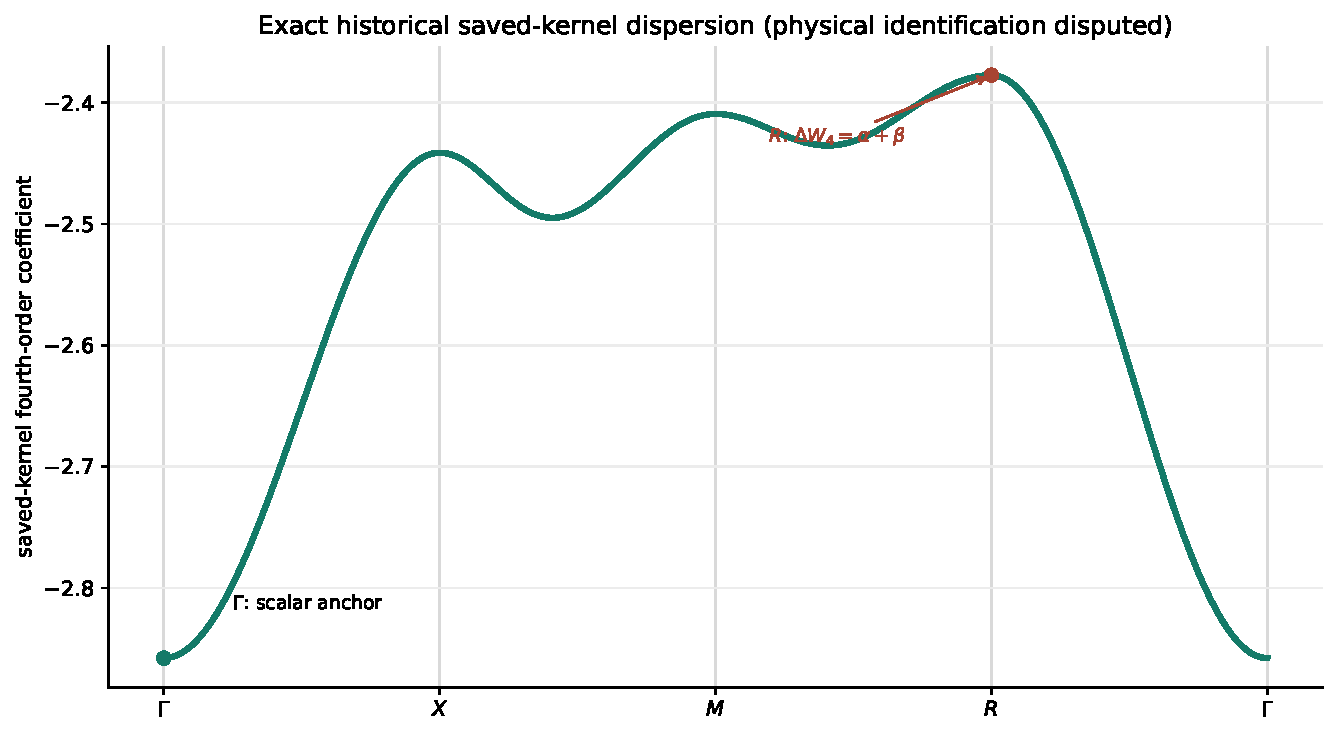
\includegraphics[width=0.94\textwidth]{figure_historical_fourth_order.pdf}
\caption{Exact dispersion of the saved historical kernel in
Reported result~\ref{rep:historical}. The plot is a theorem about that
hash-pinned kernel. Its identification with the complete physical linked
$SU(3)$ fourth-order operator is disputed, so the curve is not used as a
settled physical band.}
\label{fig:historical}
\end{figure}

The two records do agree on the axial datum, but the corpus's own quoted
tolerance does not cover that agreement: the $\alpha$ gap is
$2.43\times10^{-13}$ against a stated bound of $2.3\times10^{-13}$. The sealed core holds internally --- $\alpha_{\mathrm{new}}$ and
$4A_{\mathrm{new}}$ agree to $2\times10^{-15}$ --- which is consistent with the
quoted bound being too tight, but two float comparisons do not discriminate
that from a shared upstream slip. Recorded as a discrepancy rather than
resolved, and the bound is not widened.
\chk{v10a.26 A, B, D match the sealed rationals within 2.3e-13}
\chk{FINDING: alpha\_new falls outside the corpus's own 2.3e-13 bound}

\subsection{The obstruction is polynomial}

\begin{theorem}[Obstruction certificate]\label{thm:obstruction}
The two recorded off-axis coefficients enter \eqref{eq:shapes} only through
the shape $4e_2/q$, so the two records' carrier numerators differ by
$4\Delta_C e_2$ and their bands by $\Delta_C\,(4e_2/q)$. On any
one-dimensional axial cut two of the three $a_i$ vanish, so $e_2$ is the
\emph{zero polynomial} there and both differences vanish identically.
Consequently no $\Gamma$-point or axial datum distinguishes the two records,
at any precision. Off axis they do differ: $e_2(M)=16$ and $e_2(R)=48$, so the
numerators differ by $64\Delta_C$ and $192\Delta_C$ and the bands by
$8\Delta_C$ and $16\Delta_C$.
\end{theorem}
\chk{FINDING: the retained Gamma/axis data cannot identify C\_shp}
\chk{Phi\_C vanishes at Gamma along every direction}

\begin{remark}
The vanishing is polynomial, not numerical: this is non-identifiability, not a
limitation of the data in hand. Re-anchoring cannot substitute, and neither
record is preferred here. An off-axis contraction is the only decider.
\chk{the crosswalk is exactly scalar on the momentum axes}
\end{remark}

On the axial cut itself the invariants collapse to
$q=q_{\mathrm{ax}}(k)=4\sin^2(k/2)$ with $e_2=e_3=0$. Dividing the raw
cube-boundary numerator $(\alpha_N/4)q_{\mathrm{ax}}^2$ by
$\|w\|^2=q=q_{\mathrm{ax}}$ leaves one power of $q_{\mathrm{ax}}$ with
coefficient $\alpha_3/4=5/48$.
\chk{on an axial cut the mixed invariants vanish and the norm divides}

\subsection{A second witness}

Non-identifiability is better exhibited than argued from a difference between
two records, since a difference could always be a computational error in one of
them. The witness below is not itself a candidate for the physical
coefficient. It is the balanced continuation obtained in the supplied source
by setting an auxiliary bookkeeping parameter $\epsilon$ to zero; that source
label carries no physical meaning here. Its sole role is to make the
$4\Delta_Ce_2$ family concrete with an exactly known shift.

\begin{proposition}[Explicit second witness]\label{prop:witness}
There is a value $C_{\mathrm{alt}}$ with
$C_{\mathrm{alt}}-C_{\mathrm{old}}=25/1024$ exactly, appearing verbatim in the
pinned source edition, whose induced band separations are $0$ at $X$,
$25/128$ at $M$ and $25/64$ at $R$. It is identical to
$C_{\mathrm{old}}$ on every retained datum and distinct from it off-axis.
\end{proposition}
\chk{FINDING: an explicit second witness C\_alt exhibits the C2 non-identifiability}
\chk{the C\_alt witness IS the balanced eps-free continuation, and Delta\_C/(A/2) = 15/32}

\subsection{Where the coefficient lives}

The four checkpoint deltas are the $\Gamma$-subtracted carrier corrections
$\Delta_s=\varepsilon_4(k_s)-\varepsilon_4(0)$ at
$k_X=(\pi,0,0)$, $k_M=(\pi,\pi,0)$, $k_P=(\pi,\pi/2,0)$ and
$k_R=(\pi,\pi,\pi)$ --- $P$ is the off-axis, off-corner point that makes the
system invertible, with $a=(4,2,0)$. Its algebraic role is explicit here; no
additional provenance is inferred for that checkpoint. In the shape basis they are
\begin{equation}\label{eq:checkpoints}
\begin{aligned}
  \Delta_X&=4A,\\
  \Delta_M&=8A+16B+8C_{\mathrm{shp}},\\
  \Delta_P&=6A+8B+\tfrac{16}3C_{\mathrm{shp}},\\
  \Delta_R&=12A+48B+16C_{\mathrm{shp}}+\tfrac{16}3D,
\end{aligned}
\end{equation}
and they invert exactly, so the four shape coefficients are recoverable from
four checkpoints. $\Delta_X$ contains $A$ alone, which is why the axial cuts
agree whatever the dispute does.
\chk{checkpoint values at X, M, P, R}
\chk{the four extraction formulas invert the ansatz}
\chk{X is blind to B, C, D — it fixes A alone}

Four further measurements locate the coefficient and bound where a
disagreement could live. The distinction matters and is easy to lose: showing
where a coefficient's \emph{value} is concentrated is not by itself showing
where a \emph{discrepancy} can sit. Only the third item below does the second
thing.

\begin{enumerate}\itemsep2pt
\item \textbf{The shape fit's $C$ row sums to zero}, so no error in the
  $\Gamma$ anchoring can move $C_{\mathrm{shp}}$ at all; the recorded run's own
  re-anchoring moved it by $4.6\times10^{-15}$, as the zero row sum requires.
  A scalar shift is translation-local and changes nothing observable, which is
  why the two anchored scalars $q_{\mathrm{band}}^{(4)}$ and
  $m_\Gamma^{(4)}$ are differently anchored coordinates and not rival
  estimates.
\item \textbf{The coefficient's value is concentrated, not spread.} Six of
  the $189$ kernel records --- the normal $(0,0,1)$ shell --- carry $81\%$ of
  the total weight, while the $120$ rotation records carry $6\%$ and are $255$
  times less sensitive per record. This says where the coefficient lives, not
  yet where the two records can differ.
\item \textbf{The agreed axial coefficient pins the normal sector.} All six
  normal records share one amplitude $h$, and it sets both shapes rigidly:
  $A_{\mathrm{normal}}=-h$ while the raw normal amplitude is $2h$, which in the
  shape normalisation of \eqref{eq:shapes} is $C_{\mathrm{normal}}=h/2$, so
  \[
    C_{\mathrm{normal}}=-\tfrac12 A_{\mathrm{normal}}\quad\text{exactly.}
  \]
  (The factor of four between $2h$ and $h/2$ is the raw-to-shape conversion,
  not a discrepancy.) Granting $A=5/48$ --- which both records share --- together
  with the block decomposition, which puts $5/48+4x$ on the normal block and
  $-4x$ on the mixed one, therefore fixes $h$ and with it $81\%$ of the
  coefficient; and everything free to move without disturbing $A$ totals less
  than half the disputed gap. A rival kernel must differ \emph{structurally} in
  the $A$-carrying sector; no redistribution reaches the gap.
\item \textbf{The two kernels agree almost everywhere.} Their supports are
  identical and $144$ of $189$ records ride one common scale; the divergent
  cross sector is a single uniform ratio. The dispute is three amplitudes.
\end{enumerate}
\chk{the shape fit's C row sums to zero, so no Gamma-anchor error can move C\_shp at all}
\chk{a translation-local scalar shift changes nothing observable}
\chk{FINDING: C\_shp is carried by 6 of 189 records, not spread across the kernel}
\chk{FINDING: A = 5/48 pins the normal sector's whole C4 contribution}
\chk{C\_normal = -A\_normal/2: the agreed axial coefficient pins the normal channel}
\chk{the two 189-record kernels agree everywhere except three amplitudes, and the on-site anchor swap moves C by exactly zero}

Read together these four sharpen the target and prefer no side of it. They say
that a rival kernel must differ structurally in the $A$-carrying sector rather
than by redistribution. That is a constraint on candidates built on the
recorded $189$-record support --- which is where the measurement was made; a
kernel on a different support is not constrained by it at all. Neither record is promoted here and neither is withdrawn: the interval of
\emph{values} between them is not narrowed. What is narrowed is the class of
\emph{kernels} that can reach either end, and that constraint bears on both
records alike.

\subsection{What cannot decide it}

A large sealed sweep over $609$ marked clusters has been the standing candidate
for settling this. It cannot: its engine assembles coefficients through a
$\Gamma$-point scalar and emits no kernel block at all, and by
Theorem~\ref{thm:obstruction} $\Gamma$-point data are structurally incapable of
constraining $C_{\mathrm{shp}}$. This is a statement about the instrument, made
by reading it, not a report of a failed run.
\chk{FINDING: the marked-cluster engine emits the Gamma scalar only — a completed 609-sweep cannot decide C\_shp}

The instrument class that could eventually decide it now demonstrably
exists: the sealed radius-two delivery of Section~\ref{sec:radius2} emits a
seed-space \emph{matrix} at fifth order, not a scalar. What it lacks is
off-axis momentum --- a two-cube cluster has none --- so it too cannot
adjudicate. The requirement is now sharp on both counts: a decisive
instrument must emit more than a $\Gamma$ scalar \emph{and} resolve an
off-axis point such as $P$; the marked-cluster engine fails the first
condition, the radius-two delivery the second, and a target-blind
calculation satisfying both is exactly the next step named in the
conclusion.

\subsection{The kernel is six amplitudes}\label{sec:orbits}

Every non-axial number in the dispute has been a float, and for one reason: the
shape coefficients were obtained by fitting $\varepsilon_4$ at four points of
the zone, with condition number $45.8$. That is avoidable. Clearing the $1/q$
turns the ansatz into a linear identity between Laurent polynomials in
$z_j=e^{ik_j}$,
\[
  T(k)\;=\;\psi^{\dagger}S(k)\psi
   \;=\;c_0e_1+Ae_1^{2}+B\,e_1e_2+4C\,e_2+D\,e_3 ,
\]
with $s_j=4\sin^2(k_j/2)=2-z_j-z_j^{-1}$ and $e_r$ the elementary symmetric
functions of the $s_j$. Both sides are polynomials with rational coefficients,
so the system either has an exact solution valid on the whole zone or none at
all. For the saved historical kernel it has one, with identically vanishing
residual, and it returns $A=5/48$, $B=D=0$ and the registered $C_{\mathrm{shp}}$
as exact rationals.
\chk{the shape coefficients are solved, not fitted: A = 5/48, B = D = 0 exactly}

The decomposition makes a structure visible that the fit could not. The $189$
records carry only \emph{six} distinct weight magnitudes, and each magnitude is
one orbit of the cubic symmetry: a $132$-record skeleton at amplitude $u$; a
$12$-record same-plane $(0,1,1)$ in-plane orbit at $u_2$; a $24$-record
cross-plane orbit at $\rho$; a $12$-record same-plane nearest-neighbour in-plane
orbit at $\pi$; a $6$-record normal orbit at $\nu$; and the $3$ on-site records
at $\sigma$. Each orbit's amplitude, read off its own shape contribution, equals
the weight its records carry up to sign --- which is what makes it an amplitude
rather than a cluster.
\chk{the 189 records carry exactly six weight magnitudes}

Five of the six carrier projections then follow from the orbit's displacement
set in two lines. Writing $n$ for a plane's normal and $\{i,j\}$ for its own
axes, and using $|\psi_P|^2=s_{n(P)}$,
\[
\begin{aligned}
  \text{on-site} &: &S_P&=\sigma
     &&\longrightarrow\;\sigma\,e_1,\\
  \text{normal} &: &S_P&=\nu\,(2-s_n)
     &&\longrightarrow\;\nu\,(2e_1-e_1^{2}+2e_2),\\
  \text{in-plane} &: &S_P&=\pi\bigl((2-s_i)+(2-s_j)\bigr)
     &&\longrightarrow\;\pi\,(4e_1-2e_2),\\
  \text{doubled} &: &S_P&=u_2(2-s_i)(2-s_j)
     &&\longrightarrow\;u_2(4e_1-4e_2+3e_3),\\
  \text{rotation} &: &S_{PQ}&=-\epsilon_P\epsilon_Q\,\rho\,
        \bar d_{n(Q)}\overline{\bar d_{n(P)}}
     &&\longrightarrow\;-2\rho\,e_2,
\end{aligned}
\]
the last because the carrier annihilates the phases outright:
$T=-\rho\sum_{m\neq n}s_ms_n$. The skeleton's displacement set is larger and its
row is solved rather than read off, giving $u\,(12e_1-4e_1^{2}+12e_2-6e_3)$,
again with zero residual. Each of the six is an exact Laurent identity on that
orbit's own records.
\chk{every orbit's carrier projection is closed form in e1, e2, e3}

Collecting the six gives the whole shape table in closed form:
\[
  A=-\nu-4u,\qquad B=0,\qquad D=3u_2-6u,\qquad
  4C=2\nu-2\pi-4u_2-2\rho+12u .
\]
Two consequences are immediate. Only two orbits carry $A$, so the agreed axial
value fixes the normal amplitude outright, $\nu=-(5/48+4u)$: the normal channel
is not independently disputed, it is a consequence of $A$.
\chk{A = 5/48 forces the normal amplitude: nu = -(5/48 + 4u)}
And substituting that together with $u_2=2u$ collapses the fourth-order
off-axis coefficient to three signed numbers,
\[
  \boxed{\;C_{\mathrm{shp}}\;=\;-\tfrac{5}{96}\;-\;u\;-\;\tfrac{1}{2}(\rho+\pi)\;}
\]
which reproduces the registered value exactly. The seven-row displacement-block
ledger is a presentation of three amplitudes.
\chk{C\_shp = -5/96 - u - (rho + pi)/2, exactly}

\subsection{The tier collapse, in the orbit basis}

The two shape coefficients $B$ and $D$ vanish in the recorded kernel even
though the two-hop enumeration generates both, and the degree count does
\emph{not} forbid them. The carrier numerator reaches $a$-degree three, because
the projection contributes one further power of $a$: for any vector whose
components have squared modulus $a_i$ --- the carrier is one, in whichever of
the two equivalent labellings --- the quadratic form $\mathrm{diag}(a_i^2)$
evaluates to $\sum_i a_i^3=q^3-3qe_2+3e_3$, an explicit witness carrying a
nonzero $e_3$. An earlier degree-bound mechanism proposed for the collapse was
therefore retracted.
\chk{RETRACTED: the vertex count does NOT forbid B\_shp and D\_shp}
\chk{the vanishing coefficients are exactly the degree-3 ones}

At the level of displacement shells the vanishing looks like two integer
cancellations: every degree-three block amplitude is an integer multiple of one
raw record weight $x$, and $B=0$ reads $(+1,+1,-2)\cdot x$ while $D=0$ reads
$(-3,+6,-3)\cdot x$.
\chk{FINDING: the tier collapse is two integer cancellations at record level}
That grouping is the wrong one, and the orbit basis shows why. $B$ is the
coefficient of $e_1e_2$, and \emph{no orbit's closed form contains that
monomial}. There is nothing to cancel: $B$ is unpopulated, and needs no
mechanism at all. Inside the skeleton the four $B$-carrying displacement blocks
do cancel in $\pm$ pairs, same-plane against off-plane at the same shell and at
unit weight, which is the $(+1,+1,-2)$ above with the two cross-plane blocks
summed --- but that is an artefact of slicing one amplitude by displacement.
\chk{B = 0 is unpopulated, not cancelled}

$D$ is carried by exactly two orbits, the skeleton at $-6u$ and the doubled
orbit at $+3u_2$, and every other orbit has $D=0$. So the entire $e_3$ collapse
is the single equality
\[
  u_2=2u ,
\]
after which $D=-6u+3u_2$ vanishes for \emph{any} value of $u$. It is an
identity in one amplitude, not a numerical coincidence between sectors, and it
holds in the independently computed cold kernel too, with that kernel's own
$u$. What a mechanism has to explain is no longer two weight vectors: it is why
the same-plane $(0,1,1)$ in-plane orbit carries exactly twice the generic
weight.
\chk{the tier collapse is one identity: D = -6u + 3*u2 with u2 = 2u}

That, in turn, is not an independent coincidence. Fix a plane with own axes
$\{i,j\}$ and normal $n$, and write $X=2\cos k_i$, $Y=2\cos k_j$, $Z=2\cos k_n$.
Everything the plane sends to itself beyond nearest neighbour is sixteen
records: the $(0,0,2)$ shell at amplitude $u$, contributing $(X^2-2)+(Y^2-2)$;
the mixed $(0,1,1)$ records at $u$, contributing $(X+Y)Z$; and the in-plane
$(0,1,1)$ records at $u_2$, contributing $(u_2/u)XY$. Their sum is
\[
  u\bigl[(X+Y)(X+Y+Z)-4\bigr]
\]
\emph{if and only if} the cross term is $2XY$ --- that is, if and only if
$u_2=2u$. The doubling is the condition for the same-plane long-range symbol to
be a product rather than an inhomogeneous quadratic. With the product form,
$D=0$ holds separately in the same-plane sector and in the $96$-record
cross-plane skeleton, so neither vanishing is a cancellation between sectors at
all --- the cross-plane one because it is $-2u\,e_2(e_1-8)$ exactly, pure $e_2$
times a linear factor, which is also why it carries no $A$. What remains of the
question is one level up: why the fourth-order dynamics produces a product
there.
\chk{u2 = 2u is the cross term of a perfect square}

\subsection{Both branches in one basis}

Two things follow for the dispute itself, and neither promotes a side.

First, a caution about the $\epsilon$-free branch, recorded here because the
present authors first got it wrong. Evaluating the pinned structured $B_N$
expression at $N=3$ and comparing with $\beta$ recomputed from the raw $189$
records gives a difference of exactly $25/64$, and it is tempting to read
$C_{\mathrm{hist}}+25/1024$ as an exact balanced value of $C_{\mathrm{shp}}$.
That reading is wrong. At $N=3$ the structured expression returns exactly
$P_{17}(9)/(3R_{20}(9))$, and the source formula is stated only for $N\ge4$
with the explicit caution that it is not to be substituted at $N=3$; the
continuation route to that rank is separately closed, $D_{34}$ carrying
$(z-9)^3$ with $Q_{32}(9)\neq0$. The relation is real --- it is what
$\Delta\beta_3$ records --- but no direct balanced contraction at $N=3$ is held
here, so it is a relation among recorded quantities and not an established
branch.
\chk{RETRACTED: B\_3 - beta\_historical = 25/64 is a forbidden substitution, not an exact branch}

What the exceptional ranks do show is a pattern about the determinant sector,
and it is checked rather than asserted. At $SU(5)$ the shipped stage-1 scan
holds $895{,}524$ candidate support/output pairs with \emph{zero} determinant
sectors. At $SU(6)$ the sole determinant orbit shifts the scalar by exactly
$6/343$ at $q$, $X$, $M$ and $R$ while $A$, $B$ and the bandwidth are
unchanged. At $SU(4)$ the recorded offsets are $\Delta A_4=\Delta B_4=0$. So at
every exceptional rank where the determinant sector has been computed
independently it does not reach $B$, and $N=3$ would be the one rank where it
does. That is a pattern worth explaining. It is not a licence for the
substitution.
\chk{the SU(5) stage-1 scan is shipped: 895,524 pairs, zero determinant sectors}
\chk{the SU(6) determinant correction is exactly 6/343 and momentum-independent}
\chk{the N=3 continuation shift is exactly 25/64, with two exact corollaries}

Second, the two rival kernels are the same computation. The cold $v10a.26$
record dump has the same six orbit sizes, satisfies $u_2=2u$ and
$\nu=-(5/48+4u)$ to one part in $10^{13}$, and gives the same normalised shape
table row for row. Its skeleton unit is $4.1327437$ times the historical one,
and its $\rho$ and $\pi$ are \emph{opposite in sign}. So the free disagreement
is two sign-flipped amplitudes and one scale --- not a re-weighting, and not a
diffuse discrepancy. Six of the eighteen same-plane nearest-neighbour records
are the normal orbit, which $A=5/48$ pins identically on both sides; neither
kernel is self-refuting on its own $A$, so the comparison localises the
disagreement without deciding it.
\chk{FINDING: the cold kernel is the same six orbits with rho and pi sign-flipped}

\subsection{A \texorpdfstring{near-$\Gamma$}{near-Gamma} statement that does not adjudicate}

One quantitative fourth-order statement can be made without adjudicating
anything, because it depends on the kernel only through $\sqrt{W_4}$. Here
$W_4=\sup_k\bigl(\varepsilon_4(k)-\varepsilon_4(0)\bigr)$ is the zone spread of
the carrier-projected fourth-order correction about $\Gamma$, and
$\theta\in(0,1)$ is the fraction of the second-order isolation gap the
fourth-order spread is allowed to occupy; we take $\theta=1/2$ throughout.

What the criterion needs is a lower bound on $q$ over the region $|k|\ge r$,
and there it is sharp: writing $q=\sum_m h(k_m^2)$ with
$h(t)=2(1-\cos\sqrt t)$, the identity $(s\cos s-\sin s)'=-s\sin s\le0$ makes
$h$ concave and increasing on $[0,\pi^2]$, so the minimum over the simplex sits
at a vertex and
\begin{equation}\label{eq:qmin}
  \min_{|k|\ge r}q(k)=4\sin^2(r/2),
\end{equation}
attained on a coordinate axis. With $\tau(u)\ge t_3u^2$ for $u>0$, the
fourth-order shape terms are therefore dominated by the second-order dispersion
outside a ball of radius
$2\arcsin\bigl(u\sqrt{W_4/(\theta t_3)}\bigr)$, which is $Ku$ to leading order
with $K=\sqrt{W_4/(\theta t_3)}$: the two records give $K=10.85$ and
$K=15.06$ --- floating point, since one of the two bandwidths exists only as a
float --- and the larger bounds both, so the exclusion radius can be stated for
either record without choosing between them.

Jordan's inequality $q(k)\ge(4/\pi^2)|k|^2$ also holds on the whole zone and is
tight at $k=0$ and at the corner, but the corner is not where this bound is
used; on the axis it is loose by $\pi^2/4$, and the constants it gives,
$17.04$ and $23.66$, are exactly $\pi/2$ times the sharp ones.

It is not a bound on the open coefficient: a value of $C_{\mathrm{shp}}$
outside the two records carries its own $W_4$, and nothing here confines the
answer to the interval the records span. The statement is non-vacuous only for
$u<0.133$ at $\theta=1/2$, and that threshold is the same for both constants
--- the sharp radius reaches $\pi$ when $u\sqrt{W_4/(\theta t_3)}=1$, which is
exactly where $Ku=\pi$ for the Jordan constant, because the two bounds agree at
the zone corner. The excluded zone fraction grows as $u^3$.
\chk{Jordan bound q(k) >= (4/pi\^{}2)|k|\^{}2 holds on the whole zone}
\chk{the exact zone minimum of q on |k| >= r is 4 sin\^{}2(r/2), and Jordan overstates it by pi/2}
\chk{the criterion survives C2: K depends on the kernel only through sqrt(W\_4)}
\chk{the statement is non-vacuous only below an explicit coupling}

% The G18/G19 inserts below are received documents, input verbatim. They refer
% to one equation label and one citation key under the names used in the Rev5
% source; aliasing here keeps the received files byte-identical rather than
% editing them to match this manuscript.
%
% NOTE, for the maintainer: \cite{Yarotsky2004QP} and
% \cite{Yarotsky2006GroundStates} are resolved here to ONE entry, the CMP 261
% (2006) "Ground states in relatively bounded quantum perturbations of
% classical lattice systems", arXiv:math-ph/0412040 -- the paper the internal
% sheet-closure insert names in its own header. That identification was made
% when the inserts were merged and is not independently verified; in
% particular Yarotsky2004QP is NOT the quasi-particle paper already cited here
% as \cite{Yarotsky2004} (arXiv:math-ph/0411042), whose one-site nondegeneracy
% hypothesis this manuscript explicitly does not invoke.
\makeatletter
\providecommand{\whlabelalias}[2]{%
  \expandafter\global\expandafter\let\csname r@#1\expandafter\endcsname
  \csname r@#2\endcsname}
\providecommand{\whcitealias}[2]{%
  \expandafter\global\expandafter\let\csname b@#1\expandafter\endcsname
  \csname b@#2\endcsname}
\makeatother
\whlabelalias{eq:riesz-contour}{eq:rieszcircle}
\whcitealias{Yarotsky2006GroundStates}{Yarotsky2004QP}

\section{Infinite volume at fixed lattice spacing}\label{sec:g18}

Theorem~\ref{thm:riesz} is a finite-volume statement: it transports the
complete three-component shell through a contour whose constants are uniform
in $L$, but it says nothing about the thermodynamic limit, and its closing
remark is explicit that it supplies an interacting Riesz cluster rather than a
particle. This section closes that step at fixed spacing. The thermodynamic
ground state and infinite-volume Hamiltonian come from the quantum-perturbation
theorems of~\cite{Yarotsky2004QP} applied to the same three-link cell
decomposition as Proposition~\ref{prop:periodic-yarotsky-descent}; the
close-projection and GNS-transport chain then carries the coefficient shell
into the physical sector, and the second-order coefficient of the exact
orthonormal symbol isolates a rank-one internal sheet on every momentum ball
compactly separated from $\Gamma$.

Two boundaries survive and are stated where they arise. No rank-one separation
is claimed \emph{at} $\Gamma$, where the cubic $T_1$ triplet meets; and the
identification of the resulting semigroup with an isotropic Wilson-action
transfer matrix, together with every continuum statement, is a separate problem
taken up in Section~\ref{sec:g19}.

% Publication insert.  The main manuscript inputs this file once; it in turn
% inputs the repaired CMP(1) and internal-sheet closure files.

\subsection{Thermodynamic carrier reduction at fixed lattice spacing}
\label{sec:g18-thermodynamic-reduction}

The finite-volume Riesz island first has a thermodynamic consequence that is
strictly weaker than a particle theorem but stronger than a finite-volume rank
statement.  We isolate that projection step before proving the stronger band,
source-frame and patchwise carrier theorems below; no survival of a
finite-volume eigenvalue is silently assumed.

Let $\mathcal A_{\mathrm{loc}}$ be the local observable algebra of the
unconstrained link system on $\mathbb Z^3$.  Write
$(\mathcal H_u,\pi_u,\Omega_u)$ for the GNS triple of its interacting
ground state, and let $H_\infty(u)$ be the GNS Hamiltonian normalized by
$H_\infty(u)\Omega_u=0$.  Put
\[
 E_F=\frac83,\qquad
 I_F(u)=\left[\frac83(1-\lambda),\frac83(1+\lambda)\right],
 \qquad \lambda=27c_2|u| .
\]

\begin{proposition}[Infinite-volume external Riesz projection]
\label{prop:g18-infinite-riesz}
Assume
\[
 27|u|<c_1,\qquad \lambda<\frac1{33}.
\]
Then Theorems~2 and~3 of~\cite{Yarotsky2004QP}, applied to the same
three-link cell decomposition as Proposition~\ref{prop:periodic-yarotsky-descent},
give a translation-invariant thermodynamic ground state and a self-adjoint
$H_\infty(u)$ satisfying
\begin{equation}
 \operatorname{spec}H_\infty(u)
 \subset
 \bigcup_{a\in\operatorname{spec}H_{E,\infty}^{\rm kin}}
 [a(1-\lambda),a(1+\lambda)] .
 \label{eq:g18-infinite-enclosure}
\end{equation}
Consequently the contour $\Gamma_F$ in~\eqref{eq:riesz-contour} lies in the
resolvent set of $H_\infty(u)$ and defines
\begin{equation}
 P_{F,\infty}(u)
 =-\frac1{2\pi i}\oint_{\Gamma_F}
       (H_\infty(u)-z)^{-1}\,dz .
 \label{eq:g18-infinite-projection}
\end{equation}
The target interval is externally separated from the rest of the spectrum
by
\[
 \delta_-(u)\ge\frac{1-15\lambda}{3},\qquad
 \delta_+(u)\ge\frac{1-33\lambda}{6}.
\]
For local $A,B\in\mathcal A_{\mathrm{loc}}$, along Yarotsky's open-box
thermodynamic sequence (or a symmetry-preserving boundary sequence for which
the same common enclosure and weak-resolvent limit have separately been
proved),
\begin{equation}
 \lim_{L\to\infty}
 \langle A\Omega_L,P_{F,L}(u)B\Omega_L\rangle
 =
 \langle \pi_u(A)\Omega_u,
 P_{F,\infty}(u)\pi_u(B)\Omega_u\rangle .
 \label{eq:g18-projection-limit}
\end{equation}
The local gauge-invariant, charge-odd subspace is reducing, so all of these
statements remain true after restriction to the physical charge-odd local
GNS sector.
\end{proposition}

\begin{proof}
The rescaling and local norm estimate in
Proposition~\ref{prop:periodic-yarotsky-descent} verify the hypotheses of
\cite[Theorems~2 and~3]{Yarotsky2004QP}.  Those theorems give the weak-star
ground-state limit, the weak-resolvent limit, and the same multiplicative
spectral enclosure with the finite-volume free spectrum replaced by its
finite-support additive semigroup.  The Casimir arithmetic in the proof of
Theorem~\ref{thm:riesz-island} is unchanged for that semigroup: the nearest
free energies to $16/6$ are $14/6$ and $17/6$.  This proves the displayed
gaps and places $\Gamma_F$ in a common resolvent set.

Yarotsky's weak-resolvent convergence is initially stated for
$z\in\mathbb C\setminus\mathbb R$.  Choose one connected tubular
neighbourhood of $\Gamma_F$ disjoint from every finite- and infinite-volume
spectral enclosure.  Matrix elements of the resolvents are uniformly bounded
there by the common spectral clearance.  The normal-family theorem and the
identity theorem therefore extend their convergence to the contour.
Integrating the matrix elements around $\Gamma_F$ proves
~\eqref{eq:g18-projection-limit}.

Invariance of the thermodynamic state under finite-support gauge
transformations and charge conjugation gives their canonical GNS
implementing unitaries.  The corresponding automorphisms commute with the
dynamics, so the implementers commute with $H_\infty(u)$.  Define the physical
odd sector to be the closed cyclic subspace generated by local
gauge-invariant, charge-odd observables.  It is reducing for the Hamiltonian,
its resolvent and the contour projection, which proves the last assertion.
\end{proof}

\begin{remark}[What the enclosure alone does not say]
\label{rem:g18-projection-may-vanish}
The enclosure is one-sided: it says where spectrum may occur, not that every
free patch survives.  Thus Proposition~\ref{prop:g18-infinite-riesz} by
itself does not prove $P_{F,\infty}(u)\ne0$.  Nor does the finite-volume rank
$3L^3$ imply a nonzero matrix element against any fixed local source.  The
next two results supply the missing close-projection, totality and source
estimates; they are not consequences of the enclosure by itself.
\end{remark}

% Publication-ready replacement for the unsupported CMP(1) paragraph in
% G18_FIXED_SPACING_CARRIER_BRIDGE_INSERT.tex, lines 103--184.
% This file is input by G18_FIXED_SPACING_CARRIER_BRIDGE_INSERT.tex.

\subsubsection{Coefficient close projection and transport to the physical GNS sector}
\label{sec:g18-cmp1-complete}

We use the three-outgoing-link cell decomposition and the gap-one
normalization of Proposition~\ref{prop:periodic-yarotsky-descent}.  If
$J\Subset\mathbb Z^3$ is a nonempty exact cell support, write
$\mathcal H'_J$ for the corresponding excited tensor factor and
$H_{J,0}$ for the restriction of the free cell Hamiltonian.  Thus
\begin{equation}
 H_{J,0}\ge |J|\,1_{\mathcal H'_J}.
 \label{eq:g18-cmp1-cell-gap}
\end{equation}
The superscript minus below means both local gauge invariance and odd charge
conjugation parity.  Define
\begin{align}
 \mathcal X_0^-&=
 \left\{v=(v_J):v_J\in\mathcal H'_J,
       \ \|v\|_0:=\sum_J\|v_J\|<\infty\right\}^-,
 \label{eq:g18-cmp1-x0}\\
 \mathcal X_1^-&=
 \left\{v\in\mathcal X_0^-:v_J\in\operatorname{Dom}H_{J,0},
       \ \|v\|_1:=\sum_J\|H_{J,0}v_J\|<\infty\right\}.
 \label{eq:g18-cmp1-x1}
\end{align}
The empty coefficient is absent in the odd sector.  Consequently
\eqref{eq:g18-cmp1-cell-gap} makes $\|\cdot\|_1$ a norm, and the finite
coefficient families with entries in $\operatorname{Dom}H_{J,0}$ form a
core, denoted $\mathcal c_{00}^-$, for
\begin{equation}
 D(v_J)_J=(H_{J,0}v_J)_J,
 \qquad \operatorname{Dom}D=\mathcal X_1^-.
 \label{eq:g18-cmp1-D}
\end{equation}

\begin{lemma}[Exact-support symmetry]
\label{lem:g18-cmp1-exact-support-symmetry}
The exact-support projections commute with every local gauge
transformation and with charge conjugation.  Hence $D$, Yarotsky's
coefficient perturbation $F_u$, the free shell projection $R^-$, and the
coefficient Riesz projection $\mathcal P_u^-$ preserve
$\mathcal X_j^-$, $j=0,1$.
\end{lemma}

\begin{proof}
Let $p_x=|\Omega_x\rangle\langle\Omega_x|$ and $q_x=1-p_x$ on a grouped
cell.  In a finite box the exact-support projector is a tensor product of
$q_x$ for $x\in J$ and $p_x$ for $x\notin J$.  A gauge transformation at a
vertex acts on incident link factors by left or right regular
representations.  After the links are regrouped into cells this action still
factorizes over the cell tensor factors, and every factor fixes the constant
cell vacuum $\Omega_x$.  It therefore commutes with $p_x$, $q_x$, and every
exact-support projector.  Charge conjugation is the linkwise pullback by the
group automorphism $U\mapsto\overline U$; it also factorizes and fixes
$\Omega_x$, so the same conclusion holds.

 The free electric Hamiltonian and the plaquette interaction commute with
 these symmetries.  The symmetries fix the product vacuum and preserve the
 normalization
 $\langle\widetilde\Omega_\Lambda(u),\Omega_{\Lambda,0}\rangle=1$.
 Since the interacting ground line is unique in the small-coupling domain,
 this normalization fixes its representative and makes that representative
 invariant.  Uniqueness of the finite-volume coefficient expansion then
 implies that $D$ and $F_u$
commute with the induced coefficient actions.  Passing to Yarotsky's
thermodynamic coefficient limits preserves these commutators.  Functional
calculus for $D$ and the contour definition of $\mathcal P_u^-$ prove the
last assertion.
\end{proof}

\begin{lemma}[Unweighted coefficient close projection]
\label{lem:g18-cmp1-close-projection-complete}
Let $g=\sup_x\|\widehat\phi_x(u)\|=27|u|$.  There is a function
$a(g)\to0$ such that
\begin{equation}
 \|F_uv\|_0\le a(g)\|v\|_1,
 \qquad v\in\mathcal X_1^-.
 \label{eq:g18-cmp1-relative-bound}
\end{equation}
 Assume in addition the spectral-enclosure conditions
 \begin{equation}
  27|u|<c_1,\qquad
  \lambda:=27c_2|u|<\frac1{33}.
  \label{eq:g18-cmp1-enclosure-smallness}
 \end{equation}
 On the circle
 \begin{equation}
  \gamma_u=\{z:|z-4|=r_u\},
  \qquad r_u=\frac{1-\lambda}{8},
  \label{eq:g18-cmp1-dynamic-contour}
 \end{equation}
 put
 \begin{equation}
  R^-=-\frac1{2\pi i}\oint_{\gamma_u}(D-z)^{-1}\,dz,
  \qquad
  \mathcal P_u^-=-\frac1{2\pi i}
        \oint_{\gamma_u}(D+F_u-z)^{-1}\,dz .
  \label{eq:g18-cmp1-projections}
 \end{equation}
 If $q(g):=35a(g)<1$, then
\begin{equation}
 \boxed{\quad
 \|\mathcal P_u^--R^-\|_{\mathcal X_0^-\to\mathcal X_0^-}
 \le \kappa(g):=\frac{q(g)}{1-q(g)}.
 \quad}
 \label{eq:g18-cmp1-kappa}
\end{equation}
In particular, $\kappa(g)\to0$; after decreasing the small-coupling
interval, $\kappa(g)<1$.
\end{lemma}

\begin{proof}
Fix any $0<\rho<1$.  Yarotsky's estimate~(14), for an input of exact
support $J$, gives
\[
 \sum_K\|(F_uv_J)_K\|\rho^{-(d(K,J)+1)}
 \le C_{14}(\rho)g|J|\|v_J\|.
\]
Since the weight on the left is at least $\rho^{-1}$,
\[
 \sum_K\|(F_uv_J)_K\|
 \le \rho C_{14}(\rho)g|J|\|v_J\|
 \le \rho C_{14}(\rho)g\|H_{J,0}v_J\|.
\]
Summing the columns proves~\eqref{eq:g18-cmp1-relative-bound} with
$a(g)=\rho C_{14}(\rho)g$.  This also proves that $D+F_u$, with domain
$\mathcal X_1^-$, is closed when $a(g)<1$.

 The retained-shell gaps put $\gamma_u$ in the resolvent set of $D$ and give
 \[
  K_0:=\sup_{z\in\gamma_u}\|(D-z)^{-1}\|_{0\to0}
  \le\frac8{1-\lambda}.
 \]
 Moreover,
 \[
  D(D-z)^{-1}=1+z(D-z)^{-1},
  \qquad
  K_1:=\sup_{z\in\gamma_u}\|D(D-z)^{-1}\|_{0\to0}
  \le2+\frac{32}{1-\lambda}<35,
 \]
 because $|z|\le4+r_u$ on $\gamma_u$.  Therefore
\[
 \|F_u(D-z)^{-1}\|_{0\to0}\le a(g)K_1\le q(g).
\]
For $q(g)<1$, Yarotsky's Neumann series~(15) converges in
$\mathcal X_0^-$ and yields
\[
 \|(D+F_u-z)^{-1}-(D-z)^{-1}\|_{0\to0}
 \le K_0\frac{q(g)}{1-q(g)}.
\]
 The length of $\gamma_u$ is $2\pi r_u$, and
 $r_uK_0\le1$.  Contour integration therefore proves
 \eqref{eq:g18-cmp1-kappa}.
\end{proof}

\begin{lemma}[Finite-support shell bridge]
\label{lem:g18-cmp1-finite-support-shell-bridge}
In the physical charge-odd coefficient space,
\begin{equation}
 \operatorname{spec}(D|_{\mathcal X_0^-})\cap(-\infty,5)=\{4\},
 \qquad
 \operatorname{Ran}R^-
 =\overline{\operatorname{span}}^{\,\|\cdot\|_0}
   \{w_{x,\alpha}:x\in\mathbb Z^3,\ \alpha=1,2,3\}.
 \label{eq:g18-cmp1-free-shell-span}
\end{equation}
\end{lemma}

\begin{proof}
Let $v_J$ be a finite-support gauge-invariant, charge-odd eigen-coefficient
of rescaled electric energy below $5$.  Choose a periodic side length $L$
larger than the occupied-edge bounding box and embed the support injectively
in the $L^3$ torus, extending by the cell vacuum.  No occupied path winds
  around the torus, so the embedded coefficient belongs to the trivial
  electric one-form sector.  The retained-shell theorem then forces its energy
  to be $4$ and its energy-$4$ component to be a linear combination of odd
  elementary plaquette vectors.  The cell Laplacians have discrete Casimir
  spectrum, and energy below $5$ bounds the number of occupied cells.  Thus
  this diagonal direct sum has no additional approximate spectrum below $5$.
  Finite coefficient families are a core for
$D$, and spectral truncation in each finite tensor factor followed by
truncation in $J$ is dense in $\mathcal X_0^-$.  Applying these truncations
to the spectral projection of $D$ proves
\eqref{eq:g18-cmp1-free-shell-span}.
\end{proof}

\begin{lemma}[Coefficient totality]
\label{lem:g18-cmp1-coefficient-totality-complete}
Assume $\kappa(g)<1$.  Then
\begin{equation}
 \operatorname{Ran}\mathcal P_u^-
 =\overline{\mathcal P_u^-\operatorname{Ran}R^-}^{\,\|\cdot\|_0}.
 \label{eq:g18-cmp1-two-projection-totality}
\end{equation}
Using the finite-support retained-shell classification,
\begin{equation}
 \operatorname{Ran}\mathcal P_u^-
 =\overline{\operatorname{span}}^{\,\|\cdot\|_0}
 \{\mathcal P_u^-w_{x,\alpha}:
 x\in\mathbb Z^3,\ \alpha=1,2,3\}.
 \label{eq:g18-cmp1-seed-totality}
\end{equation}
\end{lemma}

\begin{proof}
Write $P=\mathcal P_u^-$, $R=R^-$, and $Q=1-R$.  Both $R$ and $Q$ are
blockwise orthogonal projections and hence contractions in the direct-sum
$\ell^1$ norm.  For $v\in\mathcal X_0^-$ set
\[
 y_0=Qv,
 \qquad y_{n+1}=QPy_n.
\]
Every $y_n$ lies in $\operatorname{Ran}Q$, and hence
\begin{equation}
 \|y_{n+1}\|_0
 =\|Q(P-R)y_n\|_0
 \le\kappa(g)\|y_n\|_0.
 \label{eq:g18-cmp1-geometric-irrelevant}
\end{equation}
Idempotence of $P$ gives the exact identity
\begin{equation}
 Py_n=P^2y_n=PRPy_n+PQPy_n=PRPy_n+Py_{n+1}.
 \label{eq:g18-cmp1-iteration-identity}
\end{equation}
Consequently, for every $N\ge0$,
\begin{equation}
 Pv=PRv+\sum_{n=0}^{N}PRPy_n+Py_{N+1}.
 \label{eq:g18-cmp1-iteration-finite}
\end{equation}
The last term tends to zero by
\eqref{eq:g18-cmp1-geometric-irrelevant}.  Every preceding term belongs to
$P\operatorname{Ran}R$, which proves~\eqref{eq:g18-cmp1-two-projection-totality}.
The reverse inclusion is immediate because $P$ is a projection.

 Lemma~\ref{lem:g18-cmp1-finite-support-shell-bridge} says that
 $\operatorname{Ran}R^-$ is the $\ell^1$-closed span of the
 $w_{x,\alpha}$.
Applying the bounded operator $P$ and using
\eqref{eq:g18-cmp1-two-projection-totality} proves
\eqref{eq:g18-cmp1-seed-totality}.  This is the complete version of the
iteration compressed into equations~(21)--(24) of
\cite{Yarotsky2004QP}; no one-site nondegeneracy assumption is used.
\end{proof}

\begin{lemma}[Coefficient-to-GNS transport]
\label{lem:g18-cmp1-gns-transport-complete}
 Let $\mathcal H_{u,\mathrm{phys}}^-$ be the closed local gauge-invariant,
 charge-odd cyclic subspace in the GNS representation of the thermodynamic
 ground state.  Put
 \begin{equation}
  \widehat H_\infty^-(u)=\frac32H_\infty^-(u),
  \label{eq:g18-cmp1-rescaled-H-infty}
 \end{equation}
 and let $P_{F,\infty}^-(u)$ be its shell Riesz projection on
 $\gamma_u$.  This is the same projection as the shell Riesz projection of
 $H_\infty^-(u)$, because multiplication of the Hamiltonian and contour by
 the same positive scalar does not change a spectral projection.
Then the coefficient map extends to a contraction
\begin{equation}
 \Gamma_u:\mathcal X_0^-\longrightarrow
 \mathcal H_{u,\mathrm{phys}}^-,
 \qquad
 \Gamma_uv=\pi_u\!\left(\sum_J\widehat v_J\right)\Omega_u,
 \label{eq:g18-cmp1-Gamma}
\end{equation}
and satisfies
\begin{equation}
 P_{F,\infty}^-(u)\Gamma_u
 =\Gamma_u\mathcal P_u^-.
 \label{eq:g18-cmp1-riesz-intertwining}
\end{equation}
Moreover,
\begin{equation}
 \operatorname{Ran}P_{F,\infty}^-(u)
 =\overline{\operatorname{span}}
 \{P_{F,\infty}^-(u)
       \pi_u(\widehat w_{x,\alpha})\Omega_u\}.
 \label{eq:g18-cmp1-gns-totality}
\end{equation}
No injectivity assumption on $\Gamma_u$ is required.
\end{lemma}

\begin{proof}
For a finite coefficient family,
\[
 \|\Gamma_uv\|
 \le\sum_J\|\pi_u(\widehat v_J)\Omega_u\|
 \le\sum_J\|\widehat v_J\|
 =\sum_J\|v_J\|=\|v\|_0.
\]
Thus the series in~\eqref{eq:g18-cmp1-Gamma} converges in operator norm and
$\Gamma_u$ extends by continuity to $\mathcal X_0^-$.  Exact-support
symmetry, Lemma~\ref{lem:g18-cmp1-exact-support-symmetry}, puts its range in
the physical odd sector.

 Yarotsky's equation~(18), in the present gap-one normalization, gives on the
 finite coefficient core
 \begin{equation}
  \widehat H_\infty^-(u)\Gamma_uv=\Gamma_u(D+F_u)v.
 \label{eq:g18-cmp1-generator-intertwining}
\end{equation}
Finite exact-support and local spectral truncations approximate every
$v\in\mathcal X_1^-$ in the $D$-graph norm.  The relative bound
\eqref{eq:g18-cmp1-relative-bound}, boundedness of $\Gamma_u$, and closedness
 of $\widehat H_\infty^-(u)$ therefore extend
\eqref{eq:g18-cmp1-generator-intertwining} to all of
 $\mathcal X_1^-$.  If $z$ lies on $\gamma_u$ and $a\in\mathcal X_0^-$,
apply this equality to
$v=(D+F_u-z)^{-1}a$ to obtain
\begin{equation}
  (\widehat H_\infty^-(u)-z)^{-1}\Gamma_ua
 =\Gamma_u(D+F_u-z)^{-1}a.
 \label{eq:g18-cmp1-resolvent-intertwining}
\end{equation}
Contour integration proves~\eqref{eq:g18-cmp1-riesz-intertwining}.

 It remains only to justify density in the correct sector.  The paragraph
 preceding equation~(18) of \cite{Yarotsky2004QP} states that finite linear
 combinations of creator vectors $\pi_u(\widehat v_J)\Omega_u$ are dense in
 the GNS Hilbert space.  To restrict this dense set to the physical odd
 sector, average a finite creator family over
the compact product of gauge groups at the finitely many vertices incident
to its support, and then apply $(1-C)/2$.  By
Lemma~\ref{lem:g18-cmp1-exact-support-symmetry}, this operation neither
enlarges exact support nor leaves the finite coefficient core.  Since the
corresponding Hilbert-space average is an orthogonal projection that fixes
every physical odd vector, the averaged creator families are dense in
$\mathcal H_{u,\mathrm{phys}}^-$.  Hence
\[
 \operatorname{Ran}P_{F,\infty}^-(u)
 =\overline{P_{F,\infty}^-(u)\Gamma_u\mathcal c_{00}^-}
 =\overline{\Gamma_u\mathcal P_u^-\mathcal c_{00}^-}.
\]
Now apply Lemma~\ref{lem:g18-cmp1-coefficient-totality-complete} and the
boundedness of $\Gamma_u$ to obtain
\eqref{eq:g18-cmp1-gns-totality}.
\end{proof}

\begin{corollary}[Uniform nonvanishing of each canonical seed]
\label{cor:g18-cmp1-seed-nonzero-complete}
For all sufficiently small $g$, every vector
\[
 \psi_{x,\alpha}
 =P_{F,\infty}^-(u)\pi_u(\widehat w_{x,\alpha})\Omega_u
\]
is nonzero, uniformly in $x$ and $\alpha$.
\end{corollary}

\begin{proof}
 The normalized creator has three-cell support $S_s$ and obeys
 $\widehat w_s^{\,*}\widehat w_s
 =p_{S_s}:=|\Omega_{S_s,0}\rangle\langle\Omega_{S_s,0}|\otimes I$.
 Here is the needed local product-vacuum estimate.  In a periodic volume,
 the product vacuum is a trial state, while the sum of interaction terms is
 bounded below by $-|\Lambda|g$.  Hence
 \[
  E_\Lambda(u)\le |\Lambda|g,
  \qquad
  E_\Lambda(u)\ge
  \sum_{x\in\Lambda}\langle\widehat h_x\rangle_{\Lambda,u}
       -|\Lambda|g .
 \]
 Translation invariance gives
 $\langle\widehat h_x\rangle_{\Lambda,u}\le2g$.  Since
 $1-p_x\le\widehat h_x$ and
 $1-p_{S_s}\le\sum_{x\in S_s}(1-p_x)$, every periodic subsequential limit
 obeys
 \[
  1-\omega_u(p_{S_s})\le2|S_s|g=6g.
 \]
 Yarotsky uniqueness identifies that limit with $\omega_u$.
Since $R^-w_s=w_s$, Lemma~\ref{lem:g18-cmp1-close-projection-complete} and
the contraction property of $\Gamma_u$ imply
\begin{align*}
 \|\psi_s\|
 &=\|\Gamma_u\mathcal P_u^-w_s\|\\
 &\ge \|\Gamma_uw_s\|
       -\|\Gamma_u(\mathcal P_u^--R^-)w_s\|\\
 &\ge \sqrt{1-6g}-\kappa(g).
\end{align*}
The last quantity is positive after decreasing the small-coupling interval.
\end{proof}

\begin{remark}[Scope]
\label{rem:g18-cmp1-scope-complete}
Lemmas~\ref{lem:g18-cmp1-close-projection-complete}--
\ref{lem:g18-cmp1-gns-transport-complete} close CMP(1) for the complete
three-component shell at fixed lattice spacing.  They do not identify an
individual internal dispersion sheet, an isotropic Wilson transfer-matrix
particle, or a continuum Yang--Mills particle.
\end{remark}


\begin{lemma}[Exponentially rooted shell dressing]
\label{lem:g18-rooted-shell-dressing}
Under the hypotheses of
Lemma~\ref{lem:g18-cmp1-close-projection-complete}, fix $0<\eta<1$ small
enough for Yarotsky's weighted estimate~(14).  For every seed
$s=(x,\alpha)$,
\begin{equation}
 \mathcal P_u^-w_s=w_s+c_s,\qquad
 \sum_J\eta^{-d(J,S_s)}
       \|H_{J,0}c_{s,J}\|
 \le A_\eta(g),
 \qquad A_\eta(g)\xrightarrow[g\to0]{}0 ,
 \label{eq:g18-rooted-projection}
\end{equation}
uniformly in $s$ and in finite-volume approximants.
\end{lemma}

\begin{proof}
For a root set $S$, put
\[
 \|v\|_{S,0}^{(\eta)}
 =\sum_J\eta^{-d(J,S)}\|v_J\|,
 \qquad
 \|v\|_{S,1}^{(\eta)}
 =\sum_J\eta^{-d(J,S)}\|H_{J,0}v_J\|.
\]
Yarotsky's estimate~(14), the triangle inequality
$d(K,S)\le d(K,J)+d(J,S)$, and $H_{J,0}\ge |J|$ give
\[
 \|F_uv\|_{S,0}^{(\eta)}
 \le a_\eta(g)\|v\|_{S,1}^{(\eta)},
 \qquad a_\eta(g)=\eta C_{14}(\eta)g.
\]
On the dynamic contour $\gamma_u$ of
\eqref{eq:g18-cmp1-dynamic-contour}, put
\[
 K_1=\sup_{z\in\gamma_u}
 \|D(D-z)^{-1}\|_{S,0\to S,0}<35,
 \qquad q_\eta=a_\eta(g)K_1.
\]
For $q_\eta<1$, the Neumann resolvent series converges in the rooted norm.
Since $R^-w_s=w_s$, applying $D$ to the resolvent difference and integrating
gives
\[
 A_\eta(g)\le r_uK_1\frac{q_\eta}{1-q_\eta}.
\]
This proves~\eqref{eq:g18-rooted-projection}.  The argument accepts an
arbitrary finite input support and does not use the one-site nondegeneracy
assumption of \cite[Theorem~4]{Yarotsky2004QP}.
\end{proof}

\begin{theorem}[Fixed-spacing three-component physical band and Wilson-source frame]
\label{thm:g18-fixed-spacing-band}
 Under the hypotheses of Proposition~\ref{prop:g18-infinite-riesz}, shrink
 the existential small-$|u|$ interval so that
 Lemmas~\ref{lem:g18-cmp1-close-projection-complete} and
 \ref{lem:g18-rooted-shell-dressing} hold.  In the physical charge-odd GNS
sector,
\begin{equation}
 \operatorname{Ran}P_{F,\infty}^-(u)
 \simeq \ell^2(\mathbb Z^3)\otimes\mathbb C^3
 \label{eq:g18-three-component-band}
\end{equation}
by a translation-intertwining unitary.  In this representation the
Hamiltonian is convolution by an exponentially summable Hermitian
$3\times3$ kernel, so its Bloch matrix is analytic in a complex momentum
strip.  The complete band retains the external gaps in
Proposition~\ref{prop:g18-infinite-riesz}.

More precisely, let
\[
 \psi_{x,\alpha}
 =P_{F,\infty}^-(u)\pi_u(\widehat w_{x,\alpha})\Omega_u,
 \qquad
 G_{st}=\langle\psi_s,\psi_t\rangle ,
\]
where $\widehat w_{x,\alpha}$ is the bounded rank-one plaquette creator.
For some $\mu>0$,
\begin{equation}
 \|G-I\|_{\mu,\sharp}=g_0(u)<1,\qquad
 G(k)\succeq(1-g_0(u))I_3
 \quad\hbox{for every real }k .
 \label{eq:g18-proved-canonical-frame}
\end{equation}

The same conclusion holds for the literal three-orientation Wilson
multiplication source
\[
 O^W_{x,\alpha}=\operatorname{ImTr}U_{p(x,\alpha)}.
\]
After the fixed normalization $c_W=i\sqrt2$, its projected synthesis map
$T_W$ is an isomorphism onto the band and its Gram symbol satisfies
\begin{equation}
 G_W(k)\succeq
 (1-\|G-I\|_{\mu,\sharp})
 (1-\|E\|_{\mu,\sharp})^2I_3>0
 \quad\hbox{for every real }k ,
 \label{eq:g18-wilson-frame}
\end{equation}
where $\|E\|_{\mu,\sharp}\to0$ as $u\to0$.
\end{theorem}

\begin{proof}
 Lemma~\ref{lem:g18-cmp1-gns-transport-complete} gives
 \[
 \operatorname{Ran}P_{F,\infty}^-
 =\overline{\operatorname{span}}\{\psi_{x,\alpha}\}.
\]
It remains to prove that these generators form a frame rather than merely a
dense family.

Yarotsky's cluster estimate~(16) has the form
\[
 |\omega_u(A^*B)-\omega_u(A^*)\omega_u(B)|
 \le C_0^{|I|+|J|}\tau(g)^{\operatorname{dist}(I,J)}
       \|A\|\|B\|,\qquad \tau(g)\to0 .
\]
The unit onsite gap and the variational energy-density bound also give, for
every fixed cell set $T$,
\[
 1-\omega_u(Q_T)\le2|T|g,\qquad
 |\omega_u(A)-\omega_0(A)|
 \le2\|A\|\sqrt{2|T|g}+4|T|g\|A\|.
\]
Use orthogonality of $P_{F,\infty}^-$ to expand only one Riesz mark:
\[
 G_{st}
 =\omega_u(\widehat w_s^*\widehat w_t)
  +\sum_J\omega_u(\widehat w_s^*\widehat c_{t,J}).
\]
Charge oddness kills all one-point functions and the empty coefficient.
For separated roots, the cluster estimate and
~\eqref{eq:g18-rooted-projection} give
\[
 |G_{st}-\delta_{st}|
 \le C\{\tau(g)^{R_{st}}+
 A_\eta(g)\theta^{R_{st}}\},
 \qquad \theta=\max\{C_0\eta,\tau(g)\}<1 .
\]
For the finitely many contacting roots, local vacuum continuity gives
$|G_{st}-\delta_{st}|\le C_{\rm loc}\sqrt g+A_\eta(g)$.
Choose $\eta$ first and then $g$ so that
$e^\mu C_0\eta<1$ and $e^\mu\tau(g)<1$.  The number of roots at distance
$n$ grows only quadratically, hence the exponentially weighted row and
column sums tend to zero with $g$.  This proves
~\eqref{eq:g18-proved-canonical-frame}.

The synthesis $J_P$ therefore obeys
\[
 (1-g_0)\|f\|_2^2\le\|J_Pf\|^2\le(1+g_0)\|f\|_2^2.
\]
Its range is closed and, by totality, is the whole Riesz range.  Thus
$W=J_PG^{-1/2}$ proves~\eqref{eq:g18-three-component-band}.

For completeness, the energy-kernel estimate uses no unrecorded second Riesz
mark.  In the gap-one coefficient normalization put
$\mathbb D_u=D+F_u$ and write $c_t=\mathcal P_u^-w_t-w_t$.  Since
$Dw_t=4w_t$ and $\mathbb D_u$ commutes with $\mathcal P_u^-$,
\[
 \mathbb D_u\mathcal P_u^-w_t=4w_t+k_t,
 \qquad k_t=Dc_t+F_uw_t+F_uc_t .
\]
The rooted relative bound and~\eqref{eq:g18-rooted-projection} give
\[
 \sum_J\eta^{-d(J,S_t)}\|(k_t)_J\|
 \le B_\eta(g):=A_\eta(g)+4a_\eta(g)
                  +a_\eta(g)A_\eta(g)\longrightarrow0 .
\]
The GNS intertwining~\eqref{eq:g18-cmp1-generator-intertwining} and
orthogonality of the Riesz projection give the one-mark identity
\[
 \bigl\langle\psi_s,\widehat H_\infty^-(u)\psi_t\bigr\rangle
 =\omega_u\!\left(\widehat w_s^*\,
        \widehat{\mathbb D_u\mathcal P_u^-w_t}\right),
 \qquad \widehat H_\infty^-(u)=\frac32H_\infty^-(u).
\]
Applying the same finite-contact/cluster-tail split to $4w_t+k_t$ now shows
that this energy kernel belongs to the same exponentially weighted
convolution algebra.  The convergent binomial series for $G^{-1/2}$ in that
algebra then puts $W^*H_\infty W$ there as well, proving analyticity of its
Bloch matrix.

For the literal source put
\[
 D_s=c_WO_s^W-\widehat w_s,\qquad
 M_D=3\sqrt2+1.
\]
Character orthogonality gives $c_W=i\sqrt2$ and
$D_s\Omega_0=0$.  Hence
\[
 \|\pi_u(D_s)\Omega_u\|^2
 \le6gM_D^2 .
\]
Define the three synthesis maps by
\[
 T_cf=\sum_s f_s\psi_s,
 \qquad
 T_Df=\sum_s f_sP_{F,\infty}^-(u)\pi_u(D_s)\Omega_u,
 \qquad T_W=T_c+T_D .
\]
Thus $T_W$ is exactly the projected, $c_W$-normalized literal Wilson source.
Its cross kernel is $C=T_c^*T_D$.  For contacting roots, the displayed
$O(\sqrt g)$ norm bound and Cauchy--Schwarz control $C_{st}$.  For separated
roots, use $\psi_s=\Gamma_u(w_s+c_s)$: charge oddness removes both one-point
terms, while the cluster bound controls $w_s$ and the rooted estimate controls
$c_s$.  The same contact/tail summation therefore gives
$\|C\|_{\mu,\sharp}\to0$.

Since $G=T_c^*T_c$ is invertible, put $E=G^{-1}C$.  Both $T_c$ and $T_D$ take
values in the target band, and $T_c$ is onto it.  Hence the exact identities
\[
 T_cG^{-1}T_c^*=I_{\operatorname{Ran}P_{F,\infty}^-},
 \qquad
 T_D=T_cG^{-1}T_c^*T_D=T_cE,
 \qquad
 T_W=T_c(I+E)
\]
show that $T_W$ is onto and bounded below once
$\|E\|_{\mu,\sharp}<1$.  Taking Gram matrices,
$G_W=(I+E)^*G(I+E)$, proves
~\eqref{eq:g18-wilson-frame}.
\end{proof}

\begin{remark}[Exact meaning of the closed result]
Theorem~\ref{thm:g18-fixed-spacing-band} closes the complete
three-component plaquette-shell band and the literal Wilson
\emph{source} residue at sufficiently small strong coupling and fixed
lattice spacing.  It does not isolate the one-dimensional $BB\dg$ kernel
inside each nonzero-momentum fiber, and it does not identify the Hamiltonian
semigroup with the isotropic Wilson-action transfer matrix.
\end{remark}

There is also a sharp scalar consequence for the compact carrier seed.  For an
oriented plaquette $p$, define the normalized self-adjoint charge-odd source
\[
 A_p=\frac{\chi_p-\bar\chi_p}{i\sqrt2}.
\]
Let $c_x$ be the elementary cube based at $x$, with outward incidence signs
$s(c_x,p)$, and put
\begin{equation}
 C_x=\frac1{\sqrt6}\sum_{p\subset\partial c_x}s(c_x,p)A_p,
 \qquad
 \eta_x(u)=P_{F,\infty}(u)\pi_u(C_x)\Omega_u .
 \label{eq:g18-cube-source}
\end{equation}
Its projected Gram kernel is
\begin{equation}
 G_u(x)=\langle\eta_0(u),\eta_x(u)\rangle .
 \label{eq:g18-gram-kernel}
\end{equation}
At $u=0$, plaquette orthogonality and
Proposition~\ref{prop:fixed-k-carrier} give the exact symbol
\begin{equation}
 \widehat G_0(k)=\sum_xe^{-ik\cdot x}G_0(x)=\frac{q(k)}6 .
 \label{eq:g18-free-gram}
\end{equation}

\begin{corollary}[Compact carrier-source residue]
\label{lem:g18-one-estimate}
Let $G_W(k)$ be the three-orientation literal-Wilson-source Gram symbol in
~\eqref{eq:g18-wilson-frame}.  Then the cube-boundary source
in~\eqref{eq:g18-cube-source} obeys
\begin{equation}
 \widehat G_u(k)
 \ge(1-g_0(u))
       (1-\|E\|_{\mu,\sharp})^2\frac{q(k)}6 .
 \label{eq:g18-positive-residue}
\end{equation}
In particular, on every $U\Subset\mathbb T^3\setminus\{0\}$ with
$q(k)\ge q_*>0$, the compact carrier source has residue at least
$(1-g_0(u))(1-\|E\|_{\mu,\sharp})^2q_*/6$, uniformly for $k\in U$.
\end{corollary}

\begin{proof}
In the three-orientation plaquette fiber, the normalized cube boundary has
coefficient vector $w(k)/\sqrt6$.  Theorem~\ref{thm:fact} gives
$\|w(k)\|^2=q(k)$, while the literal source in
~\eqref{eq:g18-cube-source} has the Wilson Gram, not the canonical-creator
Gram.  Equation~\eqref{eq:g18-wilson-frame} gives
$G_W(k)\succeq(1-g_0(u))(1-\|E\|_{\mu,\sharp})^2I_3$.  Therefore
\[
 \widehat G_u(k)
 =\frac16w(k)^*G_W(k)w(k)
 \ge(1-g_0(u))(1-\|E\|_{\mu,\sharp})^2\frac{q(k)}6 .
\]
\end{proof}

The full three-component band and its compact carrier-source residue are
therefore closed at fixed spacing.  The following continuation identifies the
second-order coefficient of the exact orthonormal symbol and closes its
rank-one internal sheet on every momentum ball compactly separated from
$\Gamma$.

% Publication-ready G18 continuation.  This file is input by
% G18_FIXED_SPACING_CARRIER_BRIDGE_INSERT.tex and assumes its repaired CMP(1)
% close-projection/GNS transport lemma and complete fixed-spacing
% three-component band theorem.
%
% Bibliography addition required if this insert is merged:
% \bibitem{Yarotsky2006GroundStates} D. A. Yarotsky,
%   \emph{Ground states in relatively bounded quantum perturbations of
%   classical lattice systems}, Commun. Math. Phys. \textbf{261}, 799--819
%   (2006), \href{https://arxiv.org/abs/math-ph/0412040}
%   {arXiv:math-ph/0412040}.

\subsection{Exact isolation of the internal carrier sheet away from
\texorpdfstring{$\Gamma$}{Gamma}}
\label{sec:g18-internal-sheet-closure}

This subsection works at fixed lattice spacing in the $SU(3)$ Hamiltonian
theory and in the unrescaled energy convention of Eq.~\eqref{eq:H}.  It uses
the repaired close-projection theorem and
Theorem~\ref{thm:g18-fixed-spacing-band}; no Wilson-action transfer matrix is
used.  The result closes the internal rank-one sheet on every fixed momentum
patch whose closure avoids $\Gamma$.  It does not give a gap uniform as
$k\to0$.

For $\mu>0$, let $\mathcal A_\mu$ denote the unital Banach $*$-algebra of
$3\times3$ convolution kernels $K=(K_{\alpha\beta}(x))$ on $\mathbb Z^3$ with
norm
\begin{equation}
 \|K\|_{\mu,\sharp}:=
 \max\left\{
 \max_\alpha\sum_{x,\beta}e^{\mu|x|_1}|K_{\alpha\beta}(x)|,
 \max_\beta\sum_{x,\alpha}e^{\mu|x|_1}|K_{\alpha\beta}(x)|
 \right\}.
 \label{eq:g18-weighted-algebra}
\end{equation}
Its Fourier transform is analytic for
$|\operatorname{Im}k_j|<\mu$ and
$\sup_{k\in\mathbb T^3}\|K(k)\|\le\|K\|_{\mu,\sharp}$.

\begin{lemma}[Coupling-analytic exponentially local symbol]
\label{lem:g18-u-analytic-symbol}
There are $\rho_0>0$ and $\mu>0$ such that the orthonormal-frame Hamiltonian
of Theorem~\ref{thm:g18-fixed-spacing-band} is represented by a map
\begin{equation}
 u\longmapsto h_u\in\mathcal A_\mu
 \label{eq:g18-banach-holomorphic}
\end{equation}
which is holomorphic for complex $|u|<\rho_0$.  For real $u$, $h_u(k)$ is
Hermitian.  The same statement holds for the canonical Gram kernel $G_u$ and
the physical one-mark energy kernel $\mathcal K_u$, and
\begin{equation}
 h_u=G_u^{-1/2}\mathcal K_uG_u^{-1/2}.
 \label{eq:g18-h-from-gk}
\end{equation}
Here the inverse square root is the branch satisfying $G_0^{-1/2}=I$.
\end{lemma}

\begin{proof}
Choose $\rho_0$ strictly inside both the repaired CMP(1) smallness domain and
the complex ground-state contraction domain.  With
$\lambda_0=27c_2\rho_0<1/33$, one may use the fixed contour
\[
 \gamma_{\rho_0}:\quad |z-4|=(1-\lambda_0)/8
\]
in the gap-one rescaling.  It encloses the target cluster for every
$|u|\le\rho_0$ and stays in the coefficient resolvent set.  Indeed, the
target disc has radius at most $4\lambda_0$, while the nearest other free
centres are $7/2$ and $17/4$.  The inequalities separating all three discs
from this contour reduce on the upper side to
$33\lambda_0<1$ (and on the lower side to the weaker
$\lambda_0<1/9$).  For complex $u$ this statement uses the coefficient
Neumann-resolvent bound, whose absolute majorant depends on $|u|$, rather
than a self-adjoint spectral-ordering argument.  This fixed contour, rather
than a contour depending on the evaluation point $u$, is what makes the
following holomorphic calculation literal.

The product-ground-state fixed-point map used in
\cite{Yarotsky2004QP} is analytic in the bounded interaction.  On a closed
complex $u$-disc contained in the contraction domain its contraction
constant and all coefficient majorants depend only on $|u|$.  The analytic
contraction theorem therefore makes its fixed point, the dressed coefficient
perturbation $F_u$, and the Neumann resolvent series holomorphic in their
weighted coefficient norms.  Contour integration on $\gamma_{\rho_0}$ makes
the coefficient Riesz projection $\mathcal P_u^-$ holomorphic in every
slightly weaker rooted norm.

We record why the spatial estimate remains valid on a complex disc.  In the
proof of \cite[Theorem~1]{Yarotsky2006GroundStates}, Lemmas~3--4 give
holomorphic polymer activities whose absolute values, uniformly on a closed
parameter disc, obey a majorant of the form
\[
 |a_u(\chi)|\le C_\rho\varepsilon_\rho^{|\operatorname{supp}\chi|},
 \qquad \varepsilon_\rho<1,
\]
after the coupling disc is made small enough.  The number of polymers of
size $n$ through a specified point grows at most exponentially in $n$.
Consequently the connected-cluster series is absolutely and locally
uniformly convergent for complex $u$, which is the argument used there to
prove weak-star analyticity.  With two marked local insertions, every
connected cluster joining supports $I$ and $J$ has size bounded below by a
constant times $\operatorname{dist}(I,J)$.  Summing the same activity
majorant therefore gives the complex-disc estimate
\begin{equation}
 \sup_{|u|\le\rho}
 |\omega_u^{\mathbb C}(A^*B)
   -\omega_u^{\mathbb C}(A^*)\omega_u^{\mathbb C}(B)|
 \le C_\rho^{|I|+|J|}\tau_\rho^{\operatorname{dist}(I,J)}
       \|A\|\|B\|,
 \qquad \tau_\rho<1.
 \label{eq:g18-complex-cluster-majorant}
\end{equation}
Here $\omega_u^{\mathbb C}$ denotes the holomorphic continuation; for real
$u$ it is the physical ground state.  This is an absolute cluster bound, not
an inference from real-$u$ positivity or from pointwise weak-star
analyticity.

Put $\mathbb D_u:=D+F_u$ for the gap-one coefficient Hamiltonian
and use the one-mark identities
\begin{align}
 (G_u)_{st}
 &=\omega_u\!\left(\widehat w_s^*\,\widehat{\mathcal P_u^-w_t}\right),
 \label{eq:g18-one-mark-g-analytic}\\
 (\widehat{\mathcal K}_u)_{st}
 &=\omega_u\!\left(\widehat w_s^*\,
       \widehat{\mathbb D_u\mathcal P_u^-w_t}\right),
 \qquad \mathcal K_u:=\frac23\widehat{\mathcal K}_u.
 \label{eq:g18-one-mark-k-analytic}
\end{align}
They agree with the Hilbert-space Gram and energy kernels for real $u$ but,
unlike a two-mark norm formula, also give their holomorphic continuation to
complex $u$.  To make the summation explicit, write
$\mathcal P_u^-w_t=w_t+c_t(u)$.  The rooted Neumann majorant gives, uniformly
for $|u|\le\rho<\rho_0$,
\[
 \sum_J\eta^{-d(J,S_t)}\|D_Jc_{t,J}(u)\|\le A_{\eta,\rho},
\]
and the same calculation applied to
\[
 \mathbb D_u\mathcal P_u^-w_t
 =4w_t+Dc_t+F_uw_t+F_uc_t
\]
gives a rooted majorant $A'_{\eta,\rho}$.  Both coefficient families are
holomorphic.  Exact-support projections commute with charge conjugation, so
$w_t$, $c_{t,J}$ and every displayed energy correction are charge odd.  The
analytically continued ground-state functional is charge even; hence both
one-point terms in
\eqref{eq:g18-complex-cluster-majorant} vanish identically, for complex as
well as real $u$.  For separated roots apply
\eqref{eq:g18-complex-cluster-majorant} term by term and use
$\operatorname{dist}(S_s,S_t)\le
\operatorname{dist}(S_s,J)+d(J,S_t)$, exactly as in the real CMP(3) Schur
sum.  Contacting roots form a fixed finite list and are bounded directly by
the absolutely convergent marked-cluster series.  Choose $\eta$ and then the
disc so that
$\theta_\rho:=\max\{C_\rho\eta,\tau_\rho\}<1$.  Since the number of roots at
distance $n$ grows quadratically, any
$0<\mu_0<-\log\theta_\rho$ gives constants $C,\mu_0>0$ such that
\[
 \sum_{x\in\mathbb Z^3}e^{\mu_0|x|_1}
 \sup_{|u|\le\rho}\bigl(
   |G_{\alpha\beta}(x;u)|
   +|\mathcal K_{\alpha\beta}(x;u)|
 \bigr)\le C,
 \qquad \rho<\rho_0.
\]
Finite spatial truncations are holomorphic, and this summable supremum
majorant makes them converge locally uniformly in $\mathcal A_\mu$ for any
$0<\mu<\mu_0$.  Thus $G_u$ and $\mathcal K_u$ are Banach-valued holomorphic
maps.

After shrinking $\rho_0$ if necessary,
$\|G_u-I\|_{\mu,\sharp}<1$.  The binomial series for $G_u^{-1/2}$ converges
locally uniformly in the unital Banach algebra $\mathcal A_\mu$ and is
holomorphic.  Equation~\eqref{eq:g18-h-from-gk} proves the claim.  The
coefficient calculation in the gap-one Hamiltonian
$\widehat H=(3/2)H$ would give the non-scalar coefficient
$(3/2)t_3=5/408$.  Multiplying the completed symbol by $2/3$ returns exactly
$t_3=5/612$ in the unrescaled normalization of Eq.~\eqref{eq:H}.
\end{proof}

\begin{lemma}[Finite-to-infinite second-order coefficient]
\label{lem:g18-finite-infinite-u2}
In the orthonormal frame of
Theorem~\ref{thm:g18-fixed-spacing-band},
\begin{equation}
 [u^0]h_u(k)=\frac83I_3,\qquad
 [u^1]h_u(k)=I_3,\qquad
 [u^2]h_u(k)=\sigma_2I_3+\frac5{612}B(k)B(k)^\dagger,
 \label{eq:g18-exact-infinite-u2}
\end{equation}
where $\sigma_2$ is a real scalar.  If the separate $SU(3)$ diagonal ledger
quoted in Section~\ref{sec:su3} is adopted, then $\sigma_2=11/306$; the
internal-sheet conclusion below does not use this value.
\end{lemma}

\begin{proof}
First work in a sufficiently large finite periodic box ($L\ge5$), in the
physical charge-odd trivial-flux shell, and use a fixed contour valid on a
complex $u$-disc.  Kato parallel transport gives a holomorphic intertwiner
from the free plaquette shell to the interacting Riesz island; on the real
axis it is unitary.  Differentiating its reduced operator at $u=0$ gives the ordinary
degenerate reduced-resolvent coefficient
\[
 P_-(-V)Q_-(E_{F,3}-H_E)^{-1}Q_-(-V)P_-
   -[u^2]E_{\rm vac,L}(u)I,
\]
with the conventional scalar terms absorbed into the diagonal ledger.  This
is precisely the $Q_-=1_--P_-$ prescription of Eq.~\eqref{eq:heff}, rather
than an eigenvalue-only comparison.  The retained-shell theorem,
the first-order charge/determinant census, and
Corollary~\ref{cor:assembly} therefore give
\[
 k_{L,0}=\frac83I,\qquad k_{L,1}=I,\qquad
 k_{L,2}=\sigma_{2,L}I+\frac5{612}BB^\dagger.
 \label{eq:g18-finite-kato-u2}
\]

The canonical Gram orthonormalization used to define $h_{L,u}$ is another
holomorphic intertwiner which equals the free plaquette frame at $u=0$ and
is unitary for real $u$.  The two identifications differ by a holomorphic
near-identity similarity $Z(u)$, unitary on the real axis.  If
$Z_0=I$ and
\[
 a(u)=a_0I+ua_1I+u^2a_2+\sum_{n\ge3}u^na_n,
\]
then direct expansion gives
\[
 [u^2]\,Z(u)^{-1}a(u)Z(u)=a_2;
\]
all possible frame terms are commutators with $a_0I$ or $a_1I$.  Thus the
full second-order matrix, not merely its eigenvalues, is unchanged by the
orthonormal-frame choice.  This is the point at which scalarity of both the
zeroth- and first-order coefficients is essential.

It remains to justify passage to infinite volume without confusing torus
convolution with convolution on $\mathbb Z^3$.  Let $\mathcal A_{\mu,L}$ be
the corresponding weighted convolution algebra on $\mathbb Z_L^3$, using
the torus distance, and let
\[
 (\Pi_LK)([x])=\sum_{n\in\mathbb Z^3}K(x+nL)
\]
be periodisation.  Then $\Pi_L:\mathcal A_\mu\to\mathcal A_{\mu,L}$ is a
contractive algebra homomorphism.  Let $G_{L,u}$ and
$\mathcal K_{L,u}$ be the periodic finite-volume one-mark kernels.  The
coefficient fixed-point and marked-cluster series converge term by term to
their infinite-volume series for every fixed centred displacement, locally
uniformly on a smaller complex $u$-disc.  The periodic ground-state limit is
the same state as the open-box limit because the small-perturbation ground
state is unique \cite{Yarotsky2005Uniqueness}.  This first identifies the
two limits for real $u$; local uniform holomorphy and the identity theorem
then identify their complex continuations on the common disc.

The proof of Lemma~\ref{lem:g18-u-analytic-symbol} gives the stronger bound,
uniformly in $L$,
\[
 \sum_{[x]}e^{\mu_0d_L([x],0)}
 \sup_{|u|\le\rho}
 \bigl(|G_{L,\alpha\beta}(x;u)|
       +|\mathcal K_{L,\alpha\beta}(x;u)|\bigr)\le C_\rho.
\]
Fix $0<\mu<\mu_0$.  Split the torus norm at
$d_L([x],0)=R$, with $2R<L$.  The finite part of
$G_{L,u}-\Pi_LG_u$ (and of the energy kernel) converges locally uniformly by
the preceding termwise limit.  Both tails, including every periodised image,
are at most $C_\rho e^{-(\mu_0-\mu)R}$.  Letting first $L\to\infty$ and then
$R\to\infty$ proves
\[
 \|G_{L,u}-\Pi_LG_u\|_{\mu,\sharp,L}\longrightarrow0,\qquad
 \|\mathcal K_{L,u}-\Pi_L\mathcal K_u\|_{\mu,\sharp,L}
 \longrightarrow0
\]
locally uniformly in $u$.  On a smaller disc all Gram kernels obey a common
$\|G_{L,u}-I\|_{\mu,\sharp,L}\le r_G<1$.  The binomial series is therefore
uniform in $L$, and the homomorphism property of $\Pi_L$ gives
\[
 \|h_{L,u}-\Pi_Lh_u\|_{\mu,\sharp,L}\longrightarrow0
\]
locally uniformly.  This also shows explicitly that wrap-around products in
the finite-torus inverse square root are accounted for by periodisation, not
silently identified with infinite convolution.  Cauchy's formula on any
circle inside that disc now gives
\begin{equation}
 [u^2]h_u(x) =
 \lim_{L\to\infty}[u^2]h_{L,u}(x)
 \label{eq:g18-cauchy-coefficient-limit}
\end{equation}
for each fixed displacement $x$.  This is stronger than convergence at a
few real couplings: local uniformity on a complex contour is what permits
interchanging the thermodynamic limit with Taylor-coefficient extraction.

At order two every connected process is supported on one face or on two
faces sharing one link.  Hence, once the roots and this finite process
neighbourhood fit without wrapping, the finite-volume coefficient is exactly
the infinite-lattice coefficient.  Lemma~\ref{lem:process-complete} excludes
all other off-diagonal supports, and
Theorem~\ref{thm:allrank} assigns the surviving oriented shared-link element
$t_3=5/612$.  Translation and cubic symmetry make the remaining diagonal a
scalar.  The coefficient is finite range, so the entrywise identity also
holds in every $\mathcal A_\mu$.  This proves
\eqref{eq:g18-exact-infinite-u2}.
\end{proof}

Define
\begin{equation}
 s_{\le2}(u):=\frac83+u+\sigma_2u^2,\qquad t_3:=\frac5{612}.
 \label{eq:g18-s2-definition}
\end{equation}

\begin{theorem}[Exact fixed-spacing carrier sheet on a nonzero-momentum patch]
\label{thm:g18-exact-fixed-k-carrier}
Assume the repaired CMP(1) lemma and
Theorem~\ref{thm:g18-fixed-spacing-band}.  Let $U$ be a relatively compact
open momentum ball whose closure lies in
$\mathbb T^3\setminus\{0\}$, and put
\[
 q_*:=\inf_{k\in U}q(k)>0.
\]
Then there is $u_U>0$ such that for every real
$0<|u|<u_U$ the exact infinite-volume target band over $U$ has a rank-one
analytic Riesz subbundle, descended from $\ker B(k)^\dagger$, separated from
the other two target branches by
\begin{equation}
 \operatorname{gap}_{\rm int}(k,u)
 \ge\frac12t_3u^2q_*,
 \qquad k\in U.
 \label{eq:g18-closed-internal-gap}
\end{equation}
Its direct integral is a reducing, translation-invariant subspace unitarily
equivalent to $L^2(U)$, on which translations and the Hamiltonian act as
\begin{equation}
 (T_xf)(k)=e^{ik\cdot x}f(k),
 \qquad
 (H_{\rm car}(u)f)(k)=E_{\rm car}(k,u)f(k).
 \label{eq:g18-carrier-representation-closed}
\end{equation}
The function $E_{\rm car}(k,u)$ is real analytic in $k$ on $U$.
\end{theorem}

\begin{proof}
Choose $0<r<\rho_0$ in Lemma~\ref{lem:g18-u-analytic-symbol} and set
\[
 M_r:=\sup_{|\zeta|=r}\|h_\zeta\|_{\mu,\sharp}<\infty,
 \qquad C_r:=\frac{2M_r}{r^3}.
\]
Cauchy's estimate in $\mathcal A_\mu$, followed by summing the Taylor tail,
gives for $|u|\le r/2$
\begin{equation}
 h_u(k)=s_{\le2}(u)I_3+t_3u^2B(k)B(k)^\dagger+R_u(k),
 \qquad
 \sup_{k\in\mathbb T^3}\|R_u(k)\|
 \le C_r|u|^3.
 \label{eq:g18-uniform-cubic-remainder}
\end{equation}
Indeed, the $n$th Banach-valued Taylor coefficient has norm at most
$M_rr^{-n}$, and
$\sum_{n\ge3}(|u|/r)^n\le2|u|^3/r^3$ on this disc.

One may therefore take, in addition to the smallness thresholds required by
CMP(1)--CMP(3),
\begin{equation}
 u_U:=\min\left\{\frac r2,
          \frac{t_3q_*}{4C_r}\right\}>0.
 \label{eq:g18-explicit-uU}
\end{equation}
For $0<|u|<u_U$,
\[
 \sup_{k\in U}\|R_u(k)\|
 \le\frac14t_3u^2q_*.
\]
The comparison matrix in
\eqref{eq:g18-uniform-cubic-remainder} has a simple carrier eigenvalue
$s_{\le2}(u)$ and a double eigenvalue
$s_{\le2}(u)+t_3u^2q(k)$.  Weyl's inequality separates the corresponding
exact spectral clusters by at least
\[
 t_3u^2q(k)-2\|R_u(k)\|
 \ge\frac12t_3u^2q_*.
\]
The small contour surrounding the lower cluster therefore defines a rank-one
Riesz projection analytic in $k$.  Put
$P_0(k)=v_0(k)v_0(k)^\dagger$ with
$v_0(k)=w(k)/\sqrt{q(k)}$; this is the limiting comparison projection chosen
by the $BB^\dagger$ coefficient, not a spectral projection of the triply
degenerate $u=0$ fiber.  The same Riesz estimate and
$\|R_u\|/(t_3u^2q_*)=O(|u|/q_*)$ show that, after decreasing $u_U$ if
necessary,
$\sup_{k\in U}\|P_{\rm car}(k,u)-P_0(k)\|<1/2$.  Hence
\[
 v_u(k):=\frac{P_{\rm car}(k,u)v_0(k)}
 {\|P_{\rm car}(k,u)v_0(k)\|}
\]
is a globally defined real-analytic unit section on the whole momentum ball.
Fourier direct integration gives
\eqref{eq:g18-carrier-representation-closed}; analyticity of the simple
eigenvalue follows from analyticity of the matrix symbol.
\end{proof}

\begin{corollary}[No dark carrier on a fixed momentum patch]
\label{cor:g18-no-dark-fixed-patch}
After possibly decreasing $u_U$, the rank-one sheet in
Theorem~\ref{thm:g18-exact-fixed-k-carrier} is seen uniformly by a dressed
cube-boundary Wilson source.  More precisely, put
\[
 v_0(k):=\frac{w(k)}{\sqrt{q(k)}},\qquad k\in U,
\]
and let $S_W(k,u)$ be the normalized literal-Wilson projected synthesis map
written in the orthonormal band frame, with the fixed CMP(4) normalization
chosen so that $S_W(k,0)=I_3$.  If $P_{\rm car}(k,u)$ is the exact rank-one
projection, then $u_U$ may be chosen so that
\begin{equation}
 \inf_{k\in U}
 \bigl\|P_{\rm car}(k,u)S_W(k,u)v_0(k)\bigr\|^2
 \ge\frac14,
 \qquad 0<|u|<u_U.
 \label{eq:g18-fixed-patch-carrier-overlap}
\end{equation}
The number $1/4$ is an absolute projected-norm bound for this normalized
coefficient vector, not a spectral fraction normalized by the full raw-source
covariance.  Consequently every $f\in C_c^\infty(U)$ gives a rapidly decaying
spatial smearing of the literal Wilson plaquettes, with cube-boundary
incidence, whose projection onto the exact carrier sheet is nonzero and
volume independent.
\end{corollary}

\begin{proof}
At $u=0$ the three target levels coincide, so there is no spectrally defined
rank-one carrier projection.  Instead let
$P_0(k)=v_0(k)v_0(k)^\dagger$ be the limiting comparison projection selected
by the $BB^\dagger$ coefficient.  Then
$P_0(k)S_W(k,0)v_0(k)=v_0(k)$.  The remainder estimate
\eqref{eq:g18-uniform-cubic-remainder} and the order-$u^2$ gap imply, by the
finite-dimensional Riesz-projection estimate, that
\[
 \sup_{k\in U}\|P_{\rm car}(k,u)-P_0(k)\|\longrightarrow0
 \quad (u\to0).
\]
CMP(3)--CMP(4) make this explicit.  In the notation
$W=T_cG^{-1/2}$ and $T_W=T_c(I+E)$,
\[
 S_W=W^*T_W=G^{1/2}(I+E),
\]
so $\|S_W-I\|_{\mu,\sharp}\to0$.  Therefore
\[
 \|P_{\rm car}S_Wv_0\|
 \ge1-\|P_{\rm car}-P_0\|-\|S_W-I\|.
\]
Since $\overline U$ is compact, the right-hand side is at least $1/2$ after
shrinking $u_U$.
Squaring gives \eqref{eq:g18-fixed-patch-carrier-overlap}.  Fourier transform
then turns $f\in C_c^\infty(U)$ into a rapidly decaying spatial smearing.
The identity
$f(k)v_0(k)=w(k)f(k)/\sqrt{q(k)}$ identifies its coefficients as the
cube-boundary incidence combination of the three literal Wilson plaquettes.
\end{proof}

\begin{remark}[What has and has not been closed]
\label{rem:g18-internal-sheet-firewall}
Theorem~\ref{thm:g18-exact-fixed-k-carrier} removes the two hypotheses in the
former conditional fixed-$k$ statement: it proves both the exact
orthonormal-symbol coefficient
$[u^2]h_u=\sigma_2I+(5/612)BB^\dagger$ and a remainder uniform in momentum
on a nonzero-momentum patch.  The threshold $u_U$ is
existential because the Yarotsky contraction majorants are existential, and
it necessarily deteriorates as $q_*\downarrow0$.  No rank-one separation at
$\Gamma$ is claimed; the cubic $T_1$ triplet meets there.

For every $a_t>0$, the exact Hamiltonian semigroup restricts to this subspace
as multiplication by $e^{-a_tE_{\rm car}(k,u)}$.  This does \emph{not}
identify $e^{-a_tH_\infty(u)}$ with the finite-temporal-spacing isotropic
Wilson-action transfer matrix.  The anisotropic-time/operator equivalence and
every continuum-limit statement remain separate open problems.
\end{remark}



\section{The continuum bridge, and where it is blocked}\label{sec:g19}

The previous section works at one fixed lattice spacing. The remaining step is
the continuum limit, and the first result below is that it cannot be reached by
extending the domain of Theorem~\ref{thm:riesz}: in the Hamiltonian coordinate
$u=g_H^{-4}$ an asymptotically free trajectory has $u(a)\to\infty$, while the
proved island requires $u<u_*$. The hypotheses are eventually \emph{disjoint},
so this is a theorem about the two domains rather than a caution about
extrapolating between them, and computing the existential constants would not
change it. The corollary that follows sharpens it: no nonzero finite
strong-coupling Taylor truncation yields a finite continuum mass at all.

What the section does supply is the shape of what would be needed --- the
necessary scaling law an electric-unit branch must obey, an unconditional
atom-passage proposition showing that a uniformly source-visible bottom atom
survives vague convergence without any isolation or Haag--Ruelle hypothesis,
and a reflection-positivity-preserving blocking corollary for the raw
deterministic Balaban average with reflection-adapted block and path data. A
two-point counterexample closes off the stochastic variant. The section ends by
naming the remaining object explicitly, which is a Hamiltonian--Wilson matching
package rather than a further estimate.

% G19 insertion used by the Rev5 manuscript source.

\begin{proposition}[Exact strong/weak-coupling separation]
\label{prop:g19-axis}
For $SU(3)$ the Hamiltonian coordinate of this paper is
$u=g_H^{-4}$.  Put
\[
 u_*:=\min\left\{\frac{c_1}{27},\frac{1}{891c_2}\right\},
\]
the coupling radius in Theorem~\ref{thm:riesz-island}.  If $a\downarrow0$ is
any asymptotically-free Hamiltonian trajectory with $g_H(a)\to0$, then
$u(a)\to\infty$.  In particular, there is $a_0>0$ such that
$u(a)>u_*$ for $0<a<a_0$.  No tail of a continuum trajectory therefore lies
in the proved Riesz-island domain.
\end{proposition}

\begin{proof}
The function $x\mapsto x^{-4}$ tends to infinity as $x\downarrow0$.
The eventual inequality is the definition of this limit.
\end{proof}

This is stronger than a warning about extrapolation: the hypotheses of the
fixed-cutoff theorem and of the continuum trajectory are eventually disjoint.
Numerical evaluation of the existential constants $c_1,c_2$ would not change
that fact.

\begin{conditional}[Necessary continuum scaling of an electric-unit branch]
\label{cond:g19-scaling}
Use the universal pure-gauge beta-function coefficients and the standard
two-loop lattice scaling law~\cite{GrossWilczek1973,Politzer1973,LuscherWeisz1995}.
Let
\[
 b_0=\frac{11N}{48\pi^2},\qquad
 b_1=\frac{34N^2}{3(16\pi^2)^2},\qquad
 p=\frac{b_1}{2b_0^2}=\frac{51}{121}.
\]
Assume that the Hamiltonian coupling has been matched to an
asymptotically-free Wilson scheme, including the anisotropy/time
normalisation, so that for a finite $\Lambda_H>0$
\begin{equation}\label{eq:g19-asymptotic-scaling}
 a\Lambda_H=
 \exp\!\left[-\frac{1}{2b_0g_H(a)^2}\right]
 \bigl(b_0g_H(a)^2\bigr)^{-p}[1+o(1)].
\end{equation}
Assume also that a vacuum-subtracted electric-unit excitation $E(u)$ obeys
\begin{equation}\label{eq:g19-hamiltonian-normalisation}
 aM(a)=c_Hg_H(a)^2E(u(a))[1+o(1)],\qquad c_H>0,
\end{equation}
and $M(a)\to M\in(0,\infty)$.  With $u=g_H^{-4}$, necessarily
\begin{equation}\label{eq:g19-necessary-law}
 E(u(a))=
 \frac{M}{c_H\Lambda_H}b_0^{-p}
 u(a)^{(1+p)/2}
 \exp\!\left[-\frac{\sqrt{u(a)}}{2b_0}\right][1+o(1)].
\end{equation}
For $SU(3)$ the essential exponential is
$\exp[-(8\pi^2/11)\sqrt u]$ and $(1+p)/2=86/121$.
\end{conditional}

The Hamer crosswalk printed earlier gives
$aM_{\rm phys}=(g^2/2)M_A(x)$ and
$E(u)=M_A(2u)/2$.  Hence $x=2u$ and $g=g_H$ would fix $c_H=1$,
not $1/2$: the half is already present in $E=M_A/2$.  We leave $c_H$
explicit because the upstream hostile audit still records the operator
normalisation $H=W/2$, $u=x/2$ as an asserted bridge and because the
Hamiltonian--Wilson anisotropy/time map needed at weak coupling has not been
derived.  Proving that map would set $c_H=1$ in the present convention.

\begin{proof}
Set $x=g_H^{-2}=\sqrt u$.  Equation
\eqref{eq:g19-asymptotic-scaling} gives
$a=\Lambda_H^{-1}e^{-x/(2b_0)}(x/b_0)^p[1+o(1)]$, while
\eqref{eq:g19-hamiltonian-normalisation} gives
$E=aMx/c_H[1+o(1)]$.  Substitution proves
\eqref{eq:g19-necessary-law}.
\end{proof}

\begin{corollary}[Finite Taylor data cannot supply the continuum mass]
\label{cor:g19-polynomial-obstruction}
Under the matching assumptions of Conditional result
\ref{cond:g19-scaling}, substituting any nonzero polynomial $P(u)$ for
$E(u)$ makes
\[
 \left|\frac{c_Hg_H(a)^2P(u(a))}{a}\right|\longrightarrow\infty.
\]
Thus no nonzero finite strong-coupling Taylor truncation yields a finite
continuum mass.
\end{corollary}

\begin{proof}
If $P$ has degree $d$ and leading coefficient $q_d\ne0$, then with
$x=\sqrt u$ the expression is
\[
 c_H\Lambda_Hq_db_0^p
 e^{x/(2b_0)}x^{2d-1-p}[1+o(1)].
\]
Its absolute value diverges because the exponential dominates every real
power.  The conclusion is about finite truncations, not about a
nonperturbatively continued branch.
\end{proof}

\begin{conditional}[Bare absolute-weight power counting]
\label{cond:g19-bare-residue}
Work first in a periodic box of fixed physical volume and let
\[
 \widetilde O_{a,n}=L(a)^{-3/2}\sum_x
       \operatorname{ImTr}U_{p_n(x)}
\]
be the volume-normalized zero-momentum source made from plaquettes normal to
direction $n$.  Suppose a continuum operator matching exists in the form
\begin{equation}
 \operatorname{ImTr}U_{p_n(x)}
 =a^d Z_d(a)\mathcal O_n(x)+o(a^dZ_d(a))
 \label{eq:g19-local-source-matching}
\end{equation}
in matrix elements against a fixed normalized state, and suppose the
corresponding continuum matrix element is finite.  Then
\begin{equation}
 \left|\langle\Psi,\widetilde O_{a,n}\Omega\rangle\right|^2
 =O\!\left(a^{2d-3}|Z_d(a)|^2\right).
 \label{eq:g19-overlap-power}
\end{equation}
For the charge-odd plaquette source, tracelessness and
\begin{equation}
 \operatorname{ImTr}e^{iX}
 =-\frac16\operatorname{Tr}X^3+O(\|X\|^5)
 \label{eq:g19-imtr-expansion}
\end{equation}
give $d=6$ and
$\mathcal O_n\propto d^{abc}B_n^aB_n^bB_n^c$.  Thus this state's absolute
spectral-atom weight for the unrenormalized, volume-normalized source has the
power $a^9|Z_6(a)|^2$.  If $Z_6$ contains only the usual logarithmic matching
factors, that absolute weight vanishes as $a\downarrow0$.
\end{conditional}

\begin{proof}
At fixed physical volume, $L(a)^3\asymp a^{-3}$.  Replacing the lattice sum
by its Riemann sum in~\eqref{eq:g19-local-source-matching} gives
\[
 L(a)^{-3/2}\sum_x a^dZ_d(a)\mathcal O_n(x)
 =a^{d-3/2}Z_d(a),
   \frac1{\sqrt{V}}\int_V\mathcal O_n(y)\,d^3y+o(a^{d-3/2}Z_d(a)).
\]
Squaring proves~\eqref{eq:g19-overlap-power}.  For a plaquette,
$X=a^2g_HF_{ij}+O(a^3)$; the linear term in
$\operatorname{Tr}e^{iX}$ vanishes and the first imaginary term is cubic,
which proves~\eqref{eq:g19-imtr-expansion} and $d=6$.
\end{proof}

This conditional result is an absolute-weight power count for the
volume-normalized operator $\widetilde O_{a,n}$ above; it is not a
statement about the Hilbert-normalized spectral fraction.  At fixed physical
Euclidean time the same overall operator normalization multiplies the bottom
atom and the full correlator, so it cancels from their ratio.  Consequently
the factor $a^9|Z_6(a)|^2$ alone proves neither collapse nor survival of a
normalized residue.  Smearing over a radius fixed in physical units changes
the operator and its matching factors; a uniform lower bound for the
renormalized source fraction still requires independent spectral-measure and
matching control.  Moreover, the three diagonal tensors
$d^{abc}B_n^aB_n^bB_n^c$ transform as $T_1$ under the cubic group but belong
to a symmetric rank-three continuum tensor; the label $T_1^{+-}$ alone does
not distinguish continuum spin one from spin three.  Auxiliary
$A_2^{+-}$ and $T_2^{+-}$ operators are required for that degeneracy test.
This is the standard cubic-subduction partner method used in continuum-spin
assignments~\cite{MorningstarPeardon1999,AthenodorouTeper2020}.

\begin{proposition}[Passage of a source-visible spectral atom]
\label{prop:g19-atom-passage}
Let $\mu_n$ be positive locally finite Borel measures on $[0,\infty)$,
and suppose
\[
 M_n=\inf\operatorname{supp}\mu_n\in[m_-,m_+],
 \qquad \mu_n(\{M_n\})\ge z_*>0 .
\]
Assume that the source spectral measures converge vaguely,
$\mu_n\Rightarrow\mu$.  After passage to any subsequence on which
$M_n\to M$, one has
\begin{equation}
 \operatorname{supp}\mu\subset[M,\infty),
 \qquad \mu(\{M\})\ge z_* .
 \label{eq:g19-atom-passage}
\end{equation}
Thus a uniformly source-visible bottom atom survives as a nonzero atom of
the limiting spectral measure; no isolation annulus, spin assignment, or
Haag--Ruelle hypothesis is needed for this weaker conclusion.
\end{proposition}

\begin{proof}
Compactness of $[m_-,m_+]$ supplies the stated subsequence.  If
$K\Subset[0,M)$, then $K\cap\operatorname{supp}\mu_n=\varnothing$ for all
sufficiently large $n$, and vague convergence gives $\mu(K)=0$.  Hence the
limiting support is contained in $[M,\infty)$.

For $\varepsilon>0$, choose $f_\varepsilon\in C_c([0,\infty))$ with
$0\le f_\varepsilon\le1$, equal to one on
$[M-\varepsilon/2,M+\varepsilon/2]\cap[0,\infty)$ and supported in
$[M-\varepsilon,M+\varepsilon]\cap[0,\infty)$.  Eventually
$f_\varepsilon(M_n)=1$, so positivity and vague convergence give
\[
 \int f_\varepsilon\,d\mu
 =\lim_n\int f_\varepsilon\,d\mu_n\ge z_* .
\]
Consequently
$\mu([M-\varepsilon,M+\varepsilon]\cap[0,\infty))\ge z_*$.  Continuity
from above as $\varepsilon\downarrow0$ proves
$\mu(\{M\})\ge z_*$.
\end{proof}

For a positive transfer Hamiltonian and a charge-odd source, write
\[
 C_n(t)=\int e^{-tE}\,d\mu_n(E),\qquad
 Z_n=\mu_n(\{M_n\}).
\]
Osterwalder--Schrader convergence~\cite{OsterwalderSeiler1978} strong enough
to imply vague convergence
of these source measures therefore turns a uniform lower bound on $Z_n$
and a two-sided physical bound on $M_n$ into the nonzero limiting atom in
Proposition~\ref{prop:g19-atom-passage}.  This is an exact reduction, not a
proof of either uniform bound or of the required OS convergence.

\begin{lemma}[What a finite-time correlator can certify]
\label{lem:g19-residue-bound}
Let a finite positive measure have the form
\[
 \mu=Z\delta_M+\nu,
 \qquad \operatorname{supp}\nu\subset[M+\Delta,\infty),
 \qquad \Delta>0,
\]
and put $C(t)=\int e^{-tE}\,d\mu(E)$ and $F(t)=e^{Mt}C(t)$.  Then
\begin{equation}
 Z\le F(t),
 \qquad
 Z\ge
 \frac{F(t)-e^{-\Delta t}C(0)}{1-e^{-\Delta t}} .
 \label{eq:g19-residue-bound}
\end{equation}
The second inequality may be replaced by zero when its right-hand side is
negative.
\end{lemma}

\begin{proof}
Positivity gives $F(t)\ge Z$.  The spectral gap gives
\[
 F(t)
 =Z+\int e^{-t(E-M)}\,d\nu(E)
 \le Z+e^{-\Delta t}\bigl(C(0)-Z\bigr),
\]
and rearrangement proves the lower bound.
\end{proof}

Without a gap above the atom, every finite-$t$ value of $F(t)$ is only an
upper bound on $Z$; an absolutely continuous threshold can imitate a
mass edge at finite time while having $Z=0$.  Lemma
\ref{lem:g19-residue-bound} therefore explains exactly where a uniform
external gap can enter a nonperturbative residue proof, while
Proposition~\ref{prop:g19-atom-passage} shows that isolation is not part of
the final atom-passage statement itself.

\begin{proposition}[Conditional OS gap passage]
\label{prop:g19-mosco}
Let $q_n$ be nonnegative closed forms of physical transfer Hamiltonians
$H_n$, with vacuum projections $P_n$, after isometric embedding in a common
Hilbert space.  Suppose $q_n$ Mosco-converges to the form $q$ of an
OS-reconstructed Hamiltonian $H$, $P_n\to P$ strongly,
$\operatorname{ran}P=\ker H$, and for one $m>0$ independent of $n$,
\[
 q_n[\psi]\ge m\lVert(1-P_n)\psi\rVert^2
 \quad(\psi\in D(q_n)).
\]
Then
\[
 q[\psi]\ge m\lVert(1-P)\psi\rVert^2,
 \qquad
 \operatorname{spec}(H)\subset\{0\}\cup[m,\infty).
\]
\end{proposition}

\begin{proof}
For $\psi\in D(q)$ choose a Mosco recovery sequence $\psi_n\to\psi$.
The recovery and liminf properties give $q_n[\psi_n]\to q[\psi]$.
Strong convergence of the projections gives
$(1-P_n)\psi_n\to(1-P)\psi$.  Passing to the limit proves the form bound;
the spectral inclusion follows from the spectral theorem.
\end{proof}

\begin{proposition}[Deterministic reflection-positive pushforward]
\label{prop:g19-rp-pushforward}
Let $(X,\mu,\theta;\mathcal A_+)$ be a reflected probability space with
\[
 (\Theta F)(U)=\overline{F(\theta U)},\qquad
 \int_X(\Theta F)F\,d\mu\ge0\quad(F\in\mathcal A_+).
\]
Let $(X',\theta';\mathcal A'_+)$ be a coarse reflected configuration space,
and let $P:X\to X'$ be measurable.  If
\begin{equation}
 P\theta=\theta'P\quad\mu\text{-a.e.},
 \qquad P^*\mathcal A'_+\subset\mathcal A_+,
 \label{eq:g19-rp-map}
\end{equation}
then the pushforward $P_\#\mu$ is reflection positive on
$\mathcal A'_+$.  On the gauge-invariant algebra the first equality may hold
only modulo a coarse gauge transformation.
\end{proposition}

\begin{proof}
For $F'\in\mathcal A'_+$ put $F=F'\circ P$.  Then
\[
 \int_{X'}(\Theta'F')F'\,d(P_\#\mu)
 =\int_X\overline{F'(\theta'P(U))}F'(P(U))\,d\mu(U)
 =\int_X(\Theta F)F\,d\mu\ge0.
\]
If equivariance holds modulo a coarse gauge transformation, gauge invariance
of $F'$ gives the same middle equality.
\end{proof}

\begin{corollary}[Reflection-adapted Balaban-form blocking]
\label{cor:g19-balaban-rp}
Let the Wilson measure live on a periodic lattice of even temporal extent and
be reflection positive on the gauge-invariant positive-time algebra.  Let an
odd block factor $L$ divide that extent.  Use centered $L^d$ blocks, put the
reflection plane between two adjacent layers of block centres, and choose the
reference trees and Balaban paths in reflection pairs, with reversed coarse
bonds defined by group inverse.  Then the raw deterministic Balaban-form
average of Eq.~(15) in Ref.~\cite{Balaban1985Averaging} pushes the Wilson
measure to a reflection-positive coarse measure.
\end{corollary}

\begin{proof}
Choose paths so that
\[
 \theta\Gamma_{c,x}=\Gamma_{\theta'c,\theta x},
 \qquad \Gamma_{c^{-1},x'}=\Gamma_{c,x}^{-1}.
\]
Holonomy is functorial under reflection, while logarithm and exponential
commute with unitary conjugation.  Reindexing the equal-weight average by
$x\mapsto\theta x$ proves $P(\theta U)=\theta'P(U)$ off the principal-log
branch set, which is Haar-null; Balaban's Eq.~(11) supplies gauge covariance.
For a positive coarse bond, both endpoint blocks lie wholly in the fine
positive half.  The locality statement following Eq.~(43) of
Ref.~\cite{Balaban1985Averaging} therefore gives
$P^*\mathcal A'_+\subset\mathcal A_+$.  Proposition
\ref{prop:g19-rp-pushforward} applies, using Wilson reflection positivity from
Ref.~\cite{OsterwalderSeiler1978}.
\end{proof}

The corollary proves preservation for the raw deterministic average with
reflection-adapted block and path data.  It does not cover Balaban's literal
lower-corner convention, field-dependent gauge fixing, an asymmetric
large/small-field partition, a softened stochastic constraint, or a complete
multistep effective action.  For the literal convention the finite-volume
geometry gate is now exactly
\begin{equation}
 P_{\rm CMP98}(\theta U)
 =g_\theta(U)\cdot\theta'P_{\rm CMP98}(U),
 \qquad
 \operatorname{supp}P_c\subset\Lambda_+
 \quad(c\in E'_+),
 \label{eq:g19-balaban-gate}
\end{equation}
where $g_\theta$ is the coarse gauge change induced by moving the reflected
upper-corner basepoint back to the chosen lower corner.  Block alignment by
itself does not prove Eq.~\eqref{eq:g19-balaban-gate}.

\begin{remark}[Equivariant Markov blocking is insufficient]
\label{rem:g19-markov-counterexample}
Let the fine space be one point.  On the coarse space
$X'=\{(s_-,s_+):s_\pm=\pm1\}$ with reflection
$(s_-,s_+)\mapsto(s_+,s_-)$, take the reflection-invariant law
\[
 \nu=\tfrac12\delta_{(+1,-1)}+\tfrac12\delta_{(-1,+1)}.
\]
The resulting Markov kernel is reflection equivariant and maps every
positive-time observable to a fine constant.  Nevertheless, for
$F(s_-,s_+)=s_+$,
\[
 \int(\Theta'F)F\,d\nu=\mathbb E_\nu[s_-s_+]=-1.
\]
Thus equivariance and one-sided mapping do not suffice for a stochastic
kernel.  A sufficient replacement is a reflection factorisation: there is a
one-sided $T:\mathcal A'_+\to\mathcal A_+$ such that
\[
 K\bigl((\Theta'F)G\bigr)=(\Theta TF)(TG)
 \qquad(F,G\in\mathcal A'_+).
\]
\end{remark}

The hypotheses of Proposition~\ref{prop:g19-mosco} are not supplied here.
Theorem~\ref{thm:riesz-island} controls a finite-volume cluster in a
fixed-cutoff small-$u$ domain, not the whole physical transfer Hamiltonian
along $a\downarrow0$.  The separate local weak-well expansion in the upstream
corpus also has no proved operator identity relating its $\beta_{\rm loc}$ to
$u$.  The exact next G19 object is therefore a Hamiltonian--Wilson matching
package: the physical energy prefactor, anisotropy/speed-of-light
renormalisation, $g_H$--$g_W$ scheme map, and a renormalised spectral measure
that can be followed to large $u$.  On a Balaban route this package must also
close Eq.~\eqref{eq:g19-balaban-gate} for the literal path convention and
preserve reflection positivity through every later gauge-fixing and
large/small-field operation.


\section{External comparisons}
\label{sec:external}

External results count here because they are \emph{independent} --- produced
without knowledge of this program --- not because they are published. We use
them only within the scope stated below; all normalisation conversions and
coefficient matches are calculations of this paper.

\paragraph{Hamer 1989, both sectors.} Let $a_n$ denote the coefficient of
$x^n$ in Hamer's tabulated dimensionless mass series. The $1^{+-}$ rest-frame series agrees
with $E_{\mathrm{flat}}$ at every shared order: $16/3\div2=8/3$ exactly,
$a_1=+1$, and $2a_2$, $4a_3$ matching $11/306$ and $d_3$ to $9.9\times10^{-14}$
and $1.1\times10^{-12}$. Conditional on the unsigned-symbol identification,
the $0^{++}$ series also matches the charge-even $A_1^{++}$ $\Gamma$-point
coefficients at $x^2$ and $x^3$, with the sign structure ($a_1=-1$ in the
scalar channel where the carrier's is $+1$) reproduced; the $E^{++}$ doublet is
not constrained by it, which is why Conditional result~\ref{prop:evengamma}
uses the splitting rather than the level. The conversion
$m_n=2^{n-1}a_n$ is $x=2u$ together
with Hamer's normalisation $ma=(g^2/2)M$ --- the $2^n$ from the substitution,
the half from the normalisation --- exactly, with no $4^r$ ambiguity anywhere.
Hamer states in print that his $x^3$ and $x^4$ terms disagree with the earlier
series of~\cite{KSS1976}. We report Hamer's comparison and do not independently
adjudicate the earlier coefficient table.
\chk{Hamer's 1+- series matches the C-odd Gamma-point coefficients through x\^{}3}
\chk{Hamer's 0++ series matches the C-even Gamma-point coefficients through x\^{}3}
\chk{the m\_n = 2\^{}(n-1) a\_n bridge is the x = 2u conversion}
\chk{the Hamer table is pinned, and the a\_4 agreement is primary-source}

\paragraph{The string tension.} Let $t_n$ denote the coefficient sequence in
the transcribed Kogut--Pearson--Shigemitsu $SU(3)$ table~\cite{KPS1981} ---
read here from the 1980 preprint, the journal pages themselves being unread
--- and let $\sigma_n$ denote the corresponding ledger coefficient after the
displayed convention conversion. The transcription satisfies exactly
$2^{n-1}t_n=\sigma_n$ for $n=2,\dots,5$, in the physical sign convention
$\sigma_n^{\mathrm{phys}}=(-1)^n\sigma_n^{\mathrm{raw}}$. The same series
reproduces $E_{\mathrm{flat}}$ term by term through $u^3$, including the
discriminating $u^3$ coefficient.
\chk{the KPS 1980 string-tension table equals the certified sigma series EXACTLY}
\chk{sigma\_n\^{}phys = (-1)\^{}n sigma\_n\^{}raw, and C5 is the n = 3 case}
\chk{the ratio and sigma series reproduce E\_flat exactly}

\paragraph{Euclidean series.} Historical Euclidean strong-coupling series by
M\"unster, Seo and Smit~\cite{Munster1981,Seo1982,Smit1982,Munster1983,Munster1985}
provide context only. Two printings of the same M\"unster/Seo series --- the
second erratum to~\cite{Munster1981}, which prints the definitive corrected
table and credits Ukawa and Seo~\cite{Seo1982} with locating the error, and
Smit's Table~1 scalar column~\cite{Smit1982}, which credits them --- agree
rational for rational through $u^8$. The accompanying corpus also contains an
apparent eighth-order discrepancy between the 1982 erratum and the 1985
table. Because every original table page has not been
independently re-transcribed for this paper, neither the apparent equality nor
the discrepancy is used as evidence. No Hamiltonian coefficient is inferred
from these Euclidean records.
\chk{the errata-resolved Euclidean series is doubly sourced, transcription for transcription}
\chk{FINDING: Munster's 1985 table shifts his 1982 erratum at eighth order}

\paragraph{The overlap obstruction.} Schierholz~\cite{Schierholz1988}
measured in 1988 that at $\beta=5.9$ --- in the Euclidean scaling region, not
at strong coupling --- a bare local operator carries only a couple of percent
of the state it interpolates, and gave the scaling $a^5$ for a local
dimension-four operator. Together with Brandstaeter, Kronfeld and
Schierholz~\cite{BKS1990} these document the degradation of local-operator
projection and its critical signal-to-noise scaling as the lattice spacing is
reduced. Nothing quantitative is transferred to the
present strong-coupling finite-order setting. Read only as a warning, these
results motivate posing \texttt{G18} in a smeared basis; they supply no bound
and do not identify the carrier with a physical glueball.
\chk{the overlap obstruction was published in 1988, and it scales}

\paragraph{Cross-regime discipline.} Two indexed papers declare an explicit
scope firewall and neither supplies a value here:
Davoudi--Raychowdhury--Shaw~\cite{DRS2021}, whose Hilbert-space cost comparison
is locked to $1{+}1$ dimensions with matter, and
Kadam--Raychowdhury--Stryker~\cite{KRS2023}. The rule is enforced by the
literature validator rather than recorded in prose.
\chk{a cross-regime paper never supplies a value}

\section{Scope}
\label{sec:scope}

This work does not establish a four-dimensional infinite-volume Yang--Mills
mass gap, a continuum glueball mass, convergence of the strong-coupling series
to the continuum, regulator independence of the first dispersive order, the
full $SU(3)$ fourth-order rest coefficient or off-axis shape, or an
identification of any level here with a physical glueball. Two of those
exclusions are now sharper than a disclaimer.
Section~\ref{sec:g18} \emph{does} reach infinite volume --- at one fixed
lattice spacing --- so what the first item excludes is the continuum, not the
thermodynamic limit. And the continuum exclusion is a theorem rather than a
caution: by Proposition~\ref{prop:g19-axis} the hypotheses of
Theorem~\ref{thm:riesz} and those of an asymptotically free trajectory are
eventually \emph{disjoint} in the coupling coordinate $u=g_H^{-4}$, so no tail
of a continuum trajectory lies in the proved domain and evaluating the
existential constants $c_1,c_2$ would not change that. Corollary
\ref{cor:g19-polynomial-obstruction} adds that no nonzero finite
strong-coupling truncation yields a finite continuum mass at all.
Section~\ref{sec:g19} names what would be required instead. At $\Gamma$ the
three face orbitals transform as an axial vector of the cubic group, which
with parity even and charge conjugation odd gives the retained-space label
$T_1^{+-}$; this is an operator-space assignment, not a spectral one.

The carrier is macroscopically degenerate at finite $L$. Under the
third-order factorisation input, the minimum internal separation of one sheet
from the incidence sheets is
$\Delta_L(u)=4\tau(u)\sin^2(\pi/L)+O(u^4)$, which falls as $L^{-2}$; it cannot
provide a volume-uniform contour for that single sheet over the entire
Brillouin zone. This statement must not be conflated with external isolation
of the complete electric shell. Theorem~\ref{thm:window} gives the latter a
volume-independent free margin $\CF/2$, while
Proposition~\ref{prop:locality} gives an $L$-independent internal coefficient
at every fixed nonzero nested momentum.
\chk{Delta\_L = 4 tau(u) sin\^{}2(pi/L) is positive and falls as L\^{}-2}

Three crossings are named explicitly, and none of them is made here.

\begin{proposition}[Exact reduction of the \texttt{G17} free-energy target]\label{prop:g17}
For the Euclidean $SU(3)$ Wilson plaquette density
$W_p=1-\tfrac13\operatorname{Re}\operatorname{Tr}U_p$, let
\[
  Z_\Lambda(b)=\int\exp\Bigl(-\sum_p b_pW_p\Bigr)d\mu,
  \qquad
  b_p(s)=\begin{cases}s,&p\in\Gamma,\\ \beta,&p\notin\Gamma,\end{cases}
\]
and write $Z_{\beta,\alpha,\Gamma}=Z_\Lambda(b(\alpha\beta))$ and
$Z_\beta=Z_\Lambda(b(\beta))$. Then
\begin{equation}\label{eq:g17int}
  \log\frac{Z_{\beta,\alpha,\Gamma}}{Z_\beta}
  =\int_{\alpha\beta}^{\beta}\sum_{p\in\Gamma}\langle W_p\rangle_{s,\Gamma}\,ds .
\end{equation}
Consequently the single local estimate
\begin{equation}\label{eq:g17est}
  \sup_{\Lambda,\Gamma,\,p\in\Gamma,\,s\in[\alpha\beta,\beta]}
  s\,\langle W_p\rangle_{s,\Gamma}\ \le\ C
\end{equation}
would imply the desired animal-uniform bound with
\begin{equation}\label{eq:g17bound}
  \frac{Z_{\beta,\alpha,\Gamma}}{Z_\beta}\le K_\alpha^{|\Gamma|},
  \qquad \log K_\alpha\le C\log(1/\alpha).
\end{equation}
\end{proposition}

\begin{proof}
Differentiating $\log Z_\Lambda(b(s))$ gives
$-\sum_{p\in\Gamma}\langle W_p\rangle_{s,\Gamma}$ and integration from $\beta$
down to $\alpha\beta$ proves \eqref{eq:g17int}. Under \eqref{eq:g17est}, each
summand is at most $C/s$, which proves \eqref{eq:g17bound}.
\end{proof}

\noindent The elementary pointwise estimate $0\le W_p\le3/2$ gives only
$\log K_\alpha\le\tfrac32(1-\alpha)\beta$; its growth in $\beta$ is precisely
why the uniform $C/s$ estimate remains a substantive open problem.

\begin{itemize}\itemsep2pt
\item \textbf{Finite lattice to infinite volume} requires an inhomogeneous
  Wilson free-energy bound with a useful $\log K_\alpha$ and a source-radius
  reduction. Proposition~\ref{prop:g17} turns the first item into the explicit
  one-plaquette estimate \eqref{eq:g17est}, but does not prove it; the
  source-radius theorem is also still unstated. Both are carried in the
  accompanying gap register as \texttt{G17}. The Hamiltonian Riesz island of
  Theorem~\ref{thm:riesz} belongs to small $u$ and does not prove this
  Euclidean weak-coupling bound.
\item \textbf{Protected level to particle} requires a volume-uniform overlap
  of a smeared, dressed $T_1^{+-}$ operator built on the carrier with the
  transfer-matrix spectrum, and multi-plaquette survival of the protected
  level (\texttt{G18}). The published overlap measurement of
  Section~\ref{sec:external} is why this theorem must live in the smeared
  basis. This edition now settles the free external gap, the complete
  finite-volume interacting Riesz island at existentially small $|u|$, the
  fixed-$k$ carrier, and the exact price of combining locality with sharp
  momentum. It does not prove a volume-uniform Wilson-source frame,
  infinite-volume totality, or the transfer map.
\item \textbf{Lattice to continuum} (\texttt{G19}) is untouched. Small $u$ is
  strong coupling; the continuum is the opposite end of the axis.
\end{itemize}

\noindent All three crossings are required and none is completed here. The new
window and Riesz-island theorems remove the free-spectrum obstruction and its
small-$u$ finite-volume persistence subproblem from \texttt{G18}, but they do
not promote the protected lattice cluster to an infinite-volume physical
particle.

The two former charge-odd completeness premises are now theorems.
Theorem~\ref{thm:window} proves more than shell completeness: below
$\tfrac52\CF$ the full trivial-flux electric spectrum is exactly $\{0,2\CF\}$
for every $N\ge3$ and $L\ge3$, and the range of $P_-$ is exactly the
charge-odd one-plaquette span. Lemma~\ref{lem:exhaust} proves that the only
off-diagonal second-order routes are the four adjacent shared-link channels:
disjoint exchange routes are orthogonal and the same-face route cancels. The
explicit projector matrix element \eqref{eq:channelme} then fixes their signs
and normalisations. These statements are analytic results; the finite-volume
$L=3,4,5$ enumerations in the verifier are regressions, not substitutes for
their proofs. They are new in this edition and have not yet faced external
referees; a reader auditing this paper should start there.

One earlier physical identification remains conditional.

That the complete linked charge-even Bloch symbol is the unsigned incidence
$\mathcal N(k)$ --- the signed incidence with the boundary orientations
dropped --- is not derived. The cubic and range in Section~\ref{sec:even} are
exact algebraic properties of the defined comparison operator; only their
physical charge-even interpretation, bandwidth and $\Gamma$-splitting rest on
this additional hypothesis.

\section{Evidence, authority, and reproducibility}
\label{sec:repro}

The accompanying dependency-free program
\texttt{verify\_publication\_core.py} uses exact integers and
\texttt{Fraction} arithmetic. Its thirty-eight checks are the coefficient
ledger and Weingarten sums, signed incidence and torus homology, closed-cube
shell, two-cube connected geometry and reported channel arithmetic, the
unsigned cubic, the saved historical Hodge pencil, the fourth-order
obstruction, the coupling convention, the planar closed form
\eqref{eq:planar}, and the exhaustive shared-link geometry, cycle censuses
and torus ranks through $L=5$ --- every value a \texttt{Fraction} and no
float constructed anywhere in the file.

It does \emph{not} cover the arithmetic new in this edition: the all-rank
Casimir shelf of Theorem~\ref{thm:window}, the $SU(3)$ additive-spectrum and
Riesz-contour arithmetic of Theorem~\ref{thm:riesz}, the cycle censuses those
proofs delegate to, the fixed-momentum carrier, the harmonic representatives
and the sharp zone minimum. Those are checked in the accompanying repository
instead, and each carries its own printed marker; the boundary is stated
rather than blurred, because a standalone verifier that is described as
covering more than it runs is worse than one with a stated edge. A second
program, \texttt{verify\_radius2\_report.py}, holds everything the sealed
radius-two artifact of Section~\ref{sec:radius2} can support: it is also
standard-library only (the payload is read with \texttt{zipfile} and
\texttt{struct}, and the $11\times11$ block is diagonalised by cyclic
Jacobi), but it works in floats at stated tolerances, and the two files are
kept separate precisely so that the exact one stays float-free. Neither
reconstructs the finite-precision Clebsch--Gordan inputs, replays the
third-order microscopic contractions, or chooses $C_{\mathrm{shp}}$.

Every sentence of this paper that a machine check certifies carries an
inline \texttt{\textbackslash chk} marker in the source; the markers are
extracted verbatim into Appendix~\ref{app:coverage}, so the coverage claim
is itself auditable rather than asserted. In the accompanying repository
\texttt{workhouse verify --only '<name>'} reruns any one of them alone, with
its numbers, in about a second.

That device is itself checked. A registered invariant reads every pinned
edition in \texttt{paper/} --- this one included --- resolves every printed
label against the live registry, and fails if one is renamed, deleted, or left
red. The guard is the reason this edition's labels can be trusted at all: the
same invariant read only the earliest pinned edition until this one landed,
and nineteen labels that had drifted in the intervening editions passed
unnoticed until it was made to read them all.

A few displayed objects deliberately carry no marker, because none is a result
of this program: the dimension and Casimir table \eqref{eq:table}, which is
standard $SU(N)$ representation theory; the boundary formulas of
Appendix~\ref{app:chain}, which are definitions --- what is checked there is
that they compose to zero; and Table~\ref{tab:counters}, which is provenance
about a commit rather than a claim about the physics.

\begin{table}[ht]
\centering\small
\begin{tabular}{@{}lr@{}}
\toprule
Layer & Count \\
\midrule
T0 --- Lean 4 theorems, no \texttt{sorry} & 37 \\
T1 --- exact re-derivations & 191 \\
T2 --- numerical, within a stated tolerance & 48 \\
Repository tests & 484 \\
\bottomrule
\end{tabular}
\caption{Counters at the pinned commit. The T0 row counts theorem
declarations with no \texttt{sorry}, which is a scrape of the tree;
\texttt{make lean} is what compiles them, and the standard the tree is held to
is that every axiom footprint lies in
$\{\texttt{propext},\texttt{Classical.choice},\texttt{Quot.sound}\}$. That
compilation was last run elsewhere: the environment this edition was typeset
in carries no Lean toolchain, and the row is not asserted as remeasured here.
The T1 and T2 rows are \texttt{make verify} and the test row is
\texttt{make check}. They are provenance rather than independent evidence; the
argument is above, and the checks are the checks.}
\label{tab:counters}
\end{table}

A smaller layer is proof-checked rather than merely re-derived. The Lean
development compiles the rank law with denominators cleared, $t_3=5/612$ and
$t_2=0$, the third-order ledger identity, the axial law at every exceptional
rank, the cycle count $(L^3-1)+3=L^3+2$, the four checkpoint-extraction
formulas and the deltas they invert, and four statements about the charge-even
cubic including the identity that its middle coefficient is $p^2$. It is
exact-rational and polynomial algebra, plus the trigonometric checkpoint
evaluations over $\mathbb R$ that supply those deltas --- the $\mathbb R$
section exists because the extraction theorems formalised only half a
statement without it. There is no perturbative derivation and no operator
theory. An earlier edition added that ``nothing that bears on
$C_{\mathrm{shp}}$ appears there''. That was false, and false about the one
genuinely open item here. The tree carries $C_{\mathrm{shp}}^{\mathrm{old}}$
as a rational constant, proves it from the pencil coefficients
($C=(\beta-2\alpha_3)/16$), and proof-checks the four checkpoint-extraction
formulas of Section~\ref{sec:fourth} --- which is precisely the
$C_{\mathrm{shp}}$ algebra. What remains true is the weaker and duller
statement: nothing in the Lean tree \emph{decides} between the two recorded
values, and by Theorem~\ref{thm:obstruction} nothing stated on $\Gamma$ or an
axis could.

\subsection{Claim-level evidence map}

\begin{table}[ht]
\centering
\small
\begin{tabular}{@{}p{0.29\textwidth}p{0.24\textwidth}p{0.39\textwidth}@{}}
\toprule
Claim & Status & Evidence in this edition \\
\midrule
Signed incidence spectrum and $L^3+2$ carrier
 & Proven & Analytic integer topology; exact replay \\
Adjacent all-rank coefficient $t_N$
 & Proven locally & Weingarten derivation; exact replay \\
Global order-$u^2$ torus assembly
 & Proven & Retained-shell theorem; process-completeness lemma; explicit projector matrix element \\
Uniform first electric spectral window
 & Proven & Spin-network support census; all-rank Casimir shelf; trivial one-form flux \\
$SU(3)$ all-orders finite-volume Riesz island
 & Proven, existential domain & Yarotsky enclosure; exact additive spectrum; periodic bounded-degree transport \\
Two-cube six-channel census
 & Reported numerical & Rational reconstructions; shared amplitude lineage; assembly test \\
Unsigned-incidence cubic and range
 & Proven algebraically & Exact characteristic polynomial and finite-grid replay \\
Physical charge-even identification
 & Conditional & Complete linked symbol, including vacuum route, not derived \\
$SU(3)$ factorisation through $u^3$
 & Upstream cold-exact & $251/251$ exact gates reported by the frozen authority; raw replay not bundled here \\
Historical fourth-order pencil
 & Exact for saved kernel & Hash-pinned payload and cold fixed-kernel checks \\
Complete physical fourth-order kernel
 & Disputed/open & Historical and August candidates differ off axis \\
Radius-two rational sub-block and $C_4$/$C_5$ increments
 & Reported numerical & Sealed hash-pinned artifact; stdlib float verifier at stated tolerances; detached replay of pinned parents; no odd $Q_3$ enclosure \\
Exact \texttt{G17} reduction
 & Proven reduction; estimate open & Differentiated inhomogeneous partition function; missing uniform one-plaquette bound \\
Infinite-volume particle or continuum gap
 & Open & No thermodynamic Wilson frame, transfer identification, or continuum bridge \\
\bottomrule
\end{tabular}
\caption{Truth status and evidence level are separate. ``Exact for a saved
kernel'' does not establish that kernel's physical identification.}
\label{tab:evidence}
\end{table}

\subsection{Upstream corpus and downstream verifier}

The organised \texttt{ALL THEORY} archive was consulted as
the upstream scientific corpus. Its four-document v4.3 authority stack is
frozen by byte count and SHA-256 in
\nolinkurl{export/MAN_GOV_export_manifest.csv}; all four entries were
rehashed for this edition and matched. The downstream verifier is
\href{https://github.com/ats314/WORKHOUSE}{WORKHOUSE}. Document flow is
one-way---frozen corpus to hash manifest to verifier---while verifier findings
return to review and status records. The later two-cube results are not in the
August 20 corpus and are therefore kept as later WORKHOUSE-local evidence.

The current hostile-scope audit branch is pinned at
\nolinkurl{ff9a5976a5b03cd763e3e50daf4326138770460d}. On Windows, its registry was
rerun locally: $229/230$ registered checks passed. The sole failure was the
known path-separator comparison for a restored payload; the payload hash and
all paper-relevant arithmetic checks passed. This is a platform-specific local
audit result, not a claim that the complete test suite or Lean tree was rerun.
The source-level \texttt{\string\chk} labels remain in this TeX file but are
suppressed typographically; this revised edition is not claimed to be covered
by the repository's older manuscript-label guard.

The authority files are identified by the following SHA-256 values:
\begin{itemize}
\item master v4.3:
  \nolinkurl{1f8295c3a797aeb854b4b0ca82485bd7f4a149617777d2a43fc147a4a53c26dd};
\item detailed formulas v3.1:
  \nolinkurl{924d5b26f865e33f530d166735e847b89f60df7fe363995e2788ab24e1ff4254};
\item consolidation guide v4.3:
  \nolinkurl{60b8a93c8149049f50ed3ce8e0cfd1b379723b6765f201395a2fda6c4a7e7aa7};
\item canonical source manifest v4.3:
  \nolinkurl{730bc99ed8d749de0dffbabfda85cd4512d8f7748782620b694759a03bacde05}.
\end{itemize}

\subsection{Data and code availability}

This release directory contains the TeX source, generated vector figures,
figure generator, exact verifier, build log, rendered-page audit, and a
SHA-256 manifest. The historical kernel payload used in
Reported result~\ref{rep:historical} has SHA-256
\nolinkurl{635d40fa8a5d7da841fd30f36185eb96f14ec4c040678ddd8fb010379afb2900}.
The pinned \texttt{ymcirc} $d=3$, $\mathcal B=4$ data blob is identified in
Ref.~\cite{ymcirc2026} and has SHA-256
\nolinkurl{4cad9538f2c052488556362e0cf6e4e63363e7f5801597aeab9013ef945c59dc}.
The exact stranded-flux audit source and result have SHA-256
\nolinkurl{a42800a91809a77bbd1d339ac604ea80a234eed305377bbabbf890fee98fde55}
and
\nolinkurl{d215fa1e9cd0bde0410eec16c687182c30bc62fa3f28c1445fd81e93888e1d60}.
The sealed radius-two spectrum of Section~\ref{sec:radius2} and its
certificate are bundled, with SHA-256
\nolinkurl{52a17f87d3990b234635828a0c92f73f781e9a3abec8bb3c127e990b7a717e6c}
and
\nolinkurl{b9b14d28438585fc4f7d88f96497e9c6e01d0532a8402ffd6db17258a1638c0e};
\texttt{verify\_radius2\_report.py} refuses to run against any other bytes.
The upstream release governs the wider supplement through
\texttt{two\_cube\_cutoff\_free\_radius2\_finite\_u\_spectrum\_manifest.json},
which pins twelve members --- derivation note, builder, hostile tests, six
sealed-parent files, result NPZ, certificate and detached verifier --- of
which only the two named above travelled with this edition. The two-cube build
and its finite-precision Clebsch--Gordan payloads are not reproduced by the
compact verifier; the exact statements that depend on them are labelled
reported. A durable tag or archival DOI is still needed before journal
submission.

Machine checks certify algebra relative to their definitions and inputs. They
do not replace derivations, promote numerical contractions to symbolic ones,
or certify an uncompleted off-axis contraction.

\section{Conclusion}

The strongest exact coefficient result is a finite-order operator theorem
built on a volume-uniform free spectral window: for every $N\ge3$ and periodic
$L\ge3$, the trivial-flux electric spectrum below $\tfrac52\CF$ is exactly
$\{0,2\CF\}$, the retained-shell theorem identifies the full charge-odd $2\CF$
eigenspace, the process-completeness lemma exhausts its second-order
off-diagonal routes, and the four shared-link fusion projectors give the
closed coefficient $t_N$ with the oriented cellular boundary fixing its sign
and geometry. This assembles \emph{without} a completeness hypothesis into a
homological flat carrier of dimension $L^3+2$: the flat sector is not a
fine-tuned interference band but the cycle space of the lattice two-complex,
degenerate because $\partial_2\partial_3=0$. Those proofs are the newest and
least-reviewed material here, and they deserve the reader's hardest look.

The apparent $L^{-2}$ obstruction is now localised: it is the minimum internal
sheet separation near $\Gamma$, whereas the free external shell margin is at
least $\CF/2$ and the coefficient at every fixed nonzero nested momentum is
volume-independent. The $SU(3)$ two-cube calculation supplies a nontrivial
operator-level assembly check, including channel-by-channel geometry and orbit
localisation, but shares its amplitude lineage and remains numerical at the
contraction layer.

For $SU(3)$ the analysis goes one step beyond finite order. Yarotsky's local
spectral enclosure, together with the exact additive Casimir arithmetic and a
periodic bounded-degree transport, gives an all-orders rank-$3L^3$ Riesz island
for the complete neutral charge-odd cluster whenever $27|u|<c_1$ and
$27c_2|u|<1/33$. This is a volume-uniform finite-volume statement with
existential constants. It neither isolates one internal sheet nor proves a
source-carrying thermodynamic particle. A later detached-replayed radius-two
extension adds nested finite-$u$ Ritz spectra and leading incremental
order-$u^4$ and order-$u^5$ effects; because the odd exterior action is absent,
it supplies neither a matched truncation error nor a complete fourth- or
fifth-order physical coefficient.

The unsigned-incidence cubic is exact as an algebraic comparison; its physical
charge-even identification is not assumed silently. At fourth order the saved
historical kernel has an exact positive generalized Hodge pencil and stencil,
yet the later candidate differs in an off-axis coefficient that no scalar
reanchoring, $\Gamma$ datum, or axial datum can determine. The decisive next
object is therefore one target-blind, hash-sealed calculation that returns the
rest scalar and off-axis shape from the same kernel. Independently, promoting
the finite-volume Riesz island to a thermodynamic, source-carrying multiplet
with a volume-uniform Wilson frame and a controlled transfer map is now the
precise fixed-spacing \texttt{G18} target, and Proposition~\ref{prop:g17}
isolates \texttt{G17}'s first missing estimate without pretending to prove it.
Until those steps are supplied, the operator and Riesz-island theorems are
substantial, but the physical fourth-order kernel, infinite-volume particle
interpretation, and continuum limit remain open.

\appendix

\section{Channel weights in closed form}\label{app:closed}

Substituting \eqref{eq:table} into \eqref{eq:w},
\begingroup\small
\begin{align*}
  w_{\mathbf 1}&=-\frac{2}{N(N^2-1)}, &
  w_{\Lambda^2F}&=-\frac{N-1}{(N+1)(2N-3)},\\
  w_{\mathrm{Adj}}&=-\frac{2(N^2-1)}{N(2N^2-1)}, &
  w_{\mathrm{Sym}^2F}&=-\frac{N+1}{(N-1)(2N+3)} .
\end{align*}
\endgroup
Their family sums are \eqref{eq:AN} and \eqref{eq:BN}, and the difference has
numerator $2N(N^2-4)$, which is the $SU(2)$ zero and the positivity for
$N\ge3$ at once.
\chk{the four channel weights follow from dimension and Casimir} At $N=3$:
$w_{\mathbf 1}=-1/12$, $w_{\mathrm{Adj}}=-16/51$, $w_{\Lambda^2F}=-1/6$,
$w_{\mathrm{Sym}^2F}=-2/9$, which are the four values
Reported result~\ref{rep:census} matches against \eqref{eq:census}.

\section{The Weingarten index sums}\label{app:wg}

With $\mathrm{Wg}(e)=1/(N^2-1)$ and $\mathrm{Wg}((12))=-1/(N(N^2-1))$, and
$\sigma,\tau$ running over $S_2$,
\[
  \begin{aligned}
    &\bigl\langle U_{i_1j_1}U_{i_2j_2}
       \bar U_{i'_1j'_1}\bar U_{i'_2j'_2}\bigr\rangle\\
    &\qquad=\sum_{\sigma,\tau}\mathrm{Wg}(\sigma\tau^{-1})
      \prod_a \delta_{i_ai'_{\sigma(a)}}\delta_{j_aj'_{\tau(a)}} .
  \end{aligned}
\]
Summing the delta products over all $N^4$ index quadruples,
\[
  M_{\mathrm{direct}}=\mathrm{Wg}(e)(N^4+N^2)+2\,\mathrm{Wg}((12))N^3=N^2,
\]
\[
  M_{\mathrm{cross}}=2\,\mathrm{Wg}(e)N^3+\mathrm{Wg}((12))(N^4+N^2)=N .
\]
Both are confirmed by explicit summation at $N=3,4,5$.
\chk{the shared-link weights are Weingarten, not an isotropy assumption}
The related fourth moment $\int|U_{11}|^4\,dU=2/[N(N+1)]$ is $1/6$ at $N=3$ and in particular
nonzero, which is what refuted a claimed Haar vanishing in the balanced
$(2,2)$ sector.
\chk{SU(3) Weingarten values follow from the general formula}
\chk{the fourth moment integral |U\_11|\^{}4 = 1/6 at N = 3}

\section{The \texorpdfstring{$SU(3)$}{SU(3)} coefficient ledger}\label{app:ledger}

\begin{center}
\begin{tabular}{@{}lll@{}}
\toprule
Order & Quantity & Value\\
\midrule
$u^0$ & electric plaquette & $8/3$\\
$u^1$ & scalar & $1$\\
$u^2$ & $BB\dg$ coefficient & $5/612$\\
$u^2$ & flat scalar & $11/306$\\
$u^3$ & $BB\dg$ coefficient & $1975/124848$\\
$u^3$ & per-neighbour leakage & $-12331/249696$\\
$u^3$ & flat scalar & $-109151/249696$\\
\bottomrule
\end{tabular}
\end{center}
\chk{the manuscript's SU(3) ledger is this registry, value by value}

The $u^1$ row is $SU(3)$-only rather than an $SU(3)$ specialisation: it is
$-\langle p,-|V|p,-\rangle=1$, which needs the $\epsilon$ channel and vanishes
for $N\ge4$. Of the rest, the $u^0$ row and the $u^2$ $BB\dg$ coefficient
specialise all-rank statements ($2\CF$ and $t_N$); the $u^2$ flat scalar
inherits the $SU(3)$ tower term through \eqref{eq:assembly}; and the three
$u^3$ rows are $SU(3)$-only and conditional on the supplied domino ledger,
exactly as Section~\ref{sec:su3} says.

\section{Unsigned comparison and conditional charge-even ledger}\label{app:even}

Conditional on identifying the unsigned-incidence comparison with the complete
linked charge-even symbol, the same convention, with
$\lambda\in\{12,-4\}$ and \eqref{eq:assembly}, gives:

\begin{center}
\begin{tabular}{@{}lll@{}}
\toprule
Order & Quantity & Value\\
\midrule
$u^2$ & hopping $t_{2,+}=\ell_3$ & $-11/306$\\
$u^2$ & on-site diagonal & $223/1020$\\
$u^2$ & band bottom ($\lambda=12$) & $-217/1020$\\
$u^2$ & band top ($\lambda=-4$) & $1109/3060$\\
$u^2$ & bandwidth $16|t_+|$ & $88/153$\\
$u^3$ & hopping $t_{3,+}$ & $-6335/249696$\\
$u^3$ & on-site diagonal ($\lambda=0$) & $52163/260100$\\
$u^3$ & band bottom ($\lambda=12$) & $-54049/520200$\\
$u^3$ & band top ($\lambda=-4$) & $471353/1560600$\\
\bottomrule
\end{tabular}
\end{center}

\chk{one assembly formula gives every C-even value at both orders}

Because $t_{r,+}<0$ at both orders, the $\lambda=-4$ endpoint is the band
\emph{maximum} in this sector. A certificate key naming it \texttt{bandmin} at
both orders is a naming error against its own arithmetic, recorded rather than
silently corrected.
\chk{FINDING: the certificate key 'bandmin' holds the band MAXIMUM, at both orders}

\section{Finite-volume chain calculation}\label{app:chain}

For $i<j$,
\[
  \partial_2[x;i,j]=[x+e_i;j]-[x;j]-[x+e_j;i]+[x;i],
\]
\begin{align*}
  \partial_3[x;1,2,3]=\;&[x+e_1;2,3]-[x;2,3]\\
  &-[x+e_2;1,3]+[x;1,3]\\
  &+[x+e_3;1,2]-[x;1,2].
\end{align*}
Substituting the second into the first cancels every edge pairwise, so
$\partial_2\partial_3=0$ over $\mathbb Z$.
\chk{d\_2 d\_3 = 0 on the built complex}
On the torus $\ker\partial_3$ is generated by the sum of all oriented cubes,
so $\operatorname{rank}\partial_3=L^3-1$.
\chk{rank d\_3 = L\^{}3 - 1 on the built complex}

\section{The two-cube geometry}\label{app:twocube}

The eleven oriented plaquettes of the $(3,2,2)$ prism, by base vertex and
ordered plane axes, are
\[
\begin{aligned}
&(000;12),\;(000;13),\;(000;23),\;(001;12),\\
&(010;13),\;(100;12),\;(100;13),\;(100;23),\\
&(101;12),\;(110;13),\;(200;23),
\end{aligned}
\]
with left, right and shared-face index sets
$I_L=(0,1,2,3,4,7)$, $I_R=(5,6,7,8,9,10)$, $I_F=(7)$. Building $G=BB^{\mathsf
T}$ from the oriented boundaries and applying the geometric M\"obius fold
\eqref{eq:mobius} leaves exactly four nonzero off-diagonal pairs,
$(0,5),(1,6),(3,8),(4,9)$, each equal to $-1$: four disjoint $2\times2$ blocks
and three isolated directions, which is why the spectra in
Section~\ref{sec:twocube} are closed form once the diagonals below are
supplied. The two connected diagonals are
\[
  D_{\mathcal B=6}=\tfrac1{612}\operatorname{diag}
  (-2317,-2317,-2295,-2317,-2317,
\]
\[
  \qquad -2317,-2317,0,-2317,-2317,-2295),
\]
\[
  D_{\mathcal B=4}=\operatorname{diag}
  (-\tfrac74,-\tfrac74,-\tfrac{15}4,-\tfrac74,-\tfrac74,
\]
\[
  \qquad -\tfrac74,-\tfrac74,0,-\tfrac74,-\tfrac74,-\tfrac{15}4),
\]
so both spectra are one line of arithmetic: a pair block contributes
$D_{ii}\mp c$ twice and each isolated direction its own $D_{ii}$. The $\mathcal B=4$
comparator on the same geometry gives $0$ once, $-\tfrac{15}4$ twice,
$-\tfrac{11}6$ four times, and $-\tfrac53$ four times:
the paired levels sit \emph{above} the isolated $-15/4$ pair, where at $\mathcal B=6$
they sit below it. The three isolated levels $\{-\tfrac{15}4,-\tfrac{15}4,0\}$
are identical in the two truncations, so the entire effect of the cutoff lives
in the four cross-cell blocks. That reversal is not the coefficient's sign by itself --- within a
$2\times2$ block the pair splits as $D\mp c$, which is invariant under
$c\to-c$ --- but the truncation's effect on the connected diagonal as well.
What the sign of $c$ alone does reverse is the ordering on a \emph{single}
cube, where the kernel is $\alpha I+tG$ with one diagonal and the spectrum of
$G$ fixed; that is the shell reversal the one-cube reconstructions report.
\chk{the B=4 comparator on the same geometry gives -1/12 with the reversed spectrum}

\section{Machine-check coverage}\label{app:coverage}

The paper's discipline is that a machine check, not a sentence, is the unit
of evidence. This appendix makes that auditable: every inline
\texttt{\textbackslash chk} marker in the source --- each one naming the
check that certifies the sentence it sits beside --- is extracted verbatim
by \texttt{make\_coverage.py} and printed here. A reader can therefore see
exactly which statements are covered, and, by their absence from this list,
which are not: the remaining load-bearing hypothesis of
Section~\ref{sec:scope} --- the charge-even identification --- appears
nowhere below, and that is the point.

% generated by make_coverage.py -- do not edit
The source carries 141 inline markers. Each line below is one marker, verbatim, under the section that carries it.

\begin{itemize}\footnotesize\itemsep1pt
\item[] \textbf{Introduction}
\begin{itemize}\itemsep0pt
  \item the discrete index theorem gives 0 on the signed face-edge operator, bounding nothing
\end{itemize}
\item[] \textbf{Hamiltonian and projected sector}
\begin{itemize}\itemsep0pt
  \item the printed towers are canonical-u: 4*Delta(3u/2) reproduces them verbatim
  \item the 4**r rescaling breaks the bridge: order 2 off by 16, order 3 by 64
  \item at N = 2 the C-odd hopping vanishes and the C-even one does not
  \item every nontrivial irrep clears 5/4 C\_F, except the fundamental pair
  \item the torus graph is simple, and the only short cycles are the L = 3 winding triangles
  \item every 4-cycle is an elementary face, except exactly the 3L\^{}2 straight winding loops at L = 4
  \item the SU(3) additive electric spectrum leaves 14, 16, 17 around the shell
\end{itemize}
\item[] \textbf{Oriented incidence and the exact carrier}
\begin{itemize}\itemsep0pt
  \item B B\^{}dagger = q I - d conj(d)\^{}T for the curl incidence
  \item dim Z\_2 = L\^{}3 + 2 by rank, not by re-arranging the formula
  \item cube boundaries and three wrapping sheets SPAN Z\_2
  \item the L\^{}3+2 count is chain-level, not the Bloch convention
  \item the Bloch and chain routes to the carrier agree
  \item the sheets average to harmonic representatives, and the Gamma block IS b\_2
  \item the Fourier sum of cube boundaries IS the carrier, and a local seed costs L\^{}-3
\end{itemize}
\item[] \textbf{The wrapping sheets are cycles, not harmonic --- and their
harmonic representatives}
\begin{itemize}\itemsep0pt
  \item FINDING: the wrapping sheets are cycles but NOT harmonic
  \item the sheets average to harmonic representatives, and the Gamma block IS b\_2
\end{itemize}
\item[] \textbf{Exact adjacent shared-link dynamics and global assembly}
\begin{itemize}\itemsep0pt
  \item each channel gap is C\_F + C\_R/2, and the weights sum to one
\end{itemize}
\item[] \textbf{The channel weights are a theorem}
\begin{itemize}\itemsep0pt
  \item the shared-link weights are Weingarten, not an isotropy assumption
  \item the Weingarten route is independent of the corpus
  \item the published dimension-ratio matrix element is this registry's weight formula
  \item the fourth moment integral |U\_11|\^{}4 = 1/6 at N = 3
\end{itemize}
\item[] \textbf{The off-diagonal process list is complete}
\begin{itemize}\itemsep0pt
  \item the plaquette graph is 12-regular and two faces share at most one link
  \item connected first order vanishes by inclusion-exclusion, not by cancellation of numbers
  \item the four channel weights follow from dimension and Casimir
  \item A\_N and B\_N are the channel sums, not transcriptions
\end{itemize}
\item[] \textbf{The shared-link law}
\begin{itemize}\itemsep0pt
  \item t\_N = B\_N - A\_N
  \item t\_N > 0 for N >= 3
  \item t\_2 = 0 and t\_3 = 5/612
  \item large-N expansion of t\_N through 1/N\^{}9
  \item deficit identity 1/4 - N\^{}3 t\_N
  \item N\^{}3 t\_N increases monotonically to 1/4
\end{itemize}
\item[] \textbf{The vacuum-mediated route}
\begin{itemize}\itemsep0pt
  \item ell\_N = A\_N + B\_N + 1/C\_F, the vacuum-mediated route at every rank
\end{itemize}
\item[] \textbf{Finite-volume width}
\begin{itemize}\itemsep0pt
  \item the zone maximum of q is 12 only at even L
  \item q\_min on the L-torus grid is 4 sin\^{}2(pi/L)
\end{itemize}
\item[] \textbf{The orientation signs are essential}
\begin{itemize}\itemsep0pt
  \item the two band spans ARE the two incidence spectra
\end{itemize}
\item[] \textbf{The second-order coefficient on a two-cube space}
\begin{itemize}\itemsep0pt
  \item connected first order vanishes by inclusion-exclusion, not by cancellation of numbers
  \item the connected two-cube geometry has exactly four cross-cell pairs, each -1
  \item the B=6 connected kernel is (5/612) G\_conn + diag, with the certified spectrum
  \item the certificate's own gates pass, target-blind, with the wrong-sign control rejected
  \item the B=6 six-channel census sums to the registry's own t\_3 = 5/612
  \item the B=6 six-channel census IS the Weingarten four-channel ledger, channel by channel
  \item every shared-link channel is separately proportional to the geometry, on all 56 pairs
\end{itemize}
\item[] \textbf{One truncation, two constructions}
\begin{itemize}\itemsep0pt
  \item B=6 retains every adjacent shared-link channel; B=4 provably cannot
  \item the retention rule is C2(rho) + 2 C2(3) <= B, and both retentions it decides are equalities
  \item the B=6 six-channel census IS the Weingarten four-channel ledger, channel by channel
  \item FINDING: the T1 link cutoff reverses the sign of t\_3, and 14/153 is what it omits
  \item FINDING: a full T1 = B = 4 cube Hamiltonian reproduces -1/12 and the reversed shell
  \item FINDING: the B = 6 cube flips the sign back to +5/612, closing the decisive test
  \item the B = 6 scalar misses the bridge's by exactly the same-face sextet route
\end{itemize}
\item[] \textbf{What the cutoff moves, and where}
\begin{itemize}\itemsep0pt
  \item the connected diagonal is orbit-constant, and only the transporting orbit moves
\end{itemize}
\item[] \textbf{The one-cube shell, and why its flat level cannot move}
\begin{itemize}\itemsep0pt
  \item the one-cube shell is A1 + T1 + E, and its flat level is the S\^{}2 fundamental class
  \item the certificate's finite-volume fingerprints, and 29 = L\^{}3 + 2 is the Lean cycle count
\end{itemize}
\item[] \textbf{A detached-replayed radius-two Ritz extension}
\begin{itemize}\itemsep0pt
  \item the sealed radius-two report passes its six float checks at stated tolerances
  \item the sealed radius-two report passes its six float checks at stated tolerances
  \item the sealed radius-two report passes its six float checks at stated tolerances
\end{itemize}
\item[] \textbf{The unsigned-incidence comparison operator}
\begin{itemize}\itemsep0pt
  \item the C-even characteristic polynomial is mu(mu - p)\^{}2 = 4 a\_1 a\_2 a\_3
  \item p + q = 12: one zone function runs both sectors
  \item the Bloch cubic IS the finite L = 3 and L = 4 plaquette spectrum, exactly
  \item the C-even range [-4, 12] is exact, and each edge is attained at one point only
  \item the C-even band touches its floor exactly on the three planes k\_j = pi
  \item the C-even band touches its floor exactly on the three planes k\_j = pi
  \item the C-even spectra at the four high-symmetry momenta
\end{itemize}
\item[] \textbf{Conditional charge-even assembly}
\begin{itemize}\itemsep0pt
  \item one assembly formula gives every registered band value
  \item one assembly formula gives every C-even value at both orders
  \item the plaquette graph is 12-regular and two faces share at most one link
  \item both declared coincidences, checked: one is ell\_N at all ranks, the other is bare
\end{itemize}
\item[] \textbf{Where the rest frame is not blind}
\begin{itemize}\itemsep0pt
  \item the C-even Gamma point pins t\_+, exactly where no C-odd Gamma datum can
  \item the C-even curvature is (4/3)|t\_+| at both orders, and isotropic
  \item the C-even bandwidth is 16|t\_+| at every order; the C-odd manifold width is 12|t\_-|
  \item at N = 2 the C-odd hopping vanishes and the C-even one does not
\end{itemize}
\item[] \textbf{\texorpdfstring{$SU(3)$}{SU(3)} through third order}
\begin{itemize}\itemsep0pt
  \item d\_3 = 7/32 + 12*leak\_3 - 4*b\_3
  \item leak\_3 is assembled from the domino diagonal and the vacuum piece
  \item E\_flat and t(u) carry the ledger coefficients
  \item d\_- = 1/2 + 12*leak\_2, and leak\_2 = -11/306
  \item FINDING: no Gamma-point datum can constrain the hopping
\end{itemize}
\item[] \textbf{What the homology protects}
\begin{itemize}\itemsep0pt
  \item a boundary-factorised correction shifts the carrier without dispersing it, for generic M
  \item the carrier projection is where the 1/q comes from
  \item clearing the denominator reproduces the five-element numerator basis
\end{itemize}
\item[] \textbf{An exact theorem for the saved historical kernel}
\begin{itemize}\itemsep0pt
  \item v10a.26 A, B, D match the sealed rationals within 2.3e-13
  \item FINDING: alpha\_new falls outside the corpus's own 2.3e-13 bound
\end{itemize}
\item[] \textbf{The obstruction is polynomial}
\begin{itemize}\itemsep0pt
  \item FINDING: the retained Gamma/axis data cannot identify C\_shp
  \item Phi\_C vanishes at Gamma along every direction
  \item the crosswalk is exactly scalar on the momentum axes
  \item on an axial cut the mixed invariants vanish and the norm divides
\end{itemize}
\item[] \textbf{A second witness}
\begin{itemize}\itemsep0pt
  \item FINDING: an explicit second witness C\_alt exhibits the C2 non-identifiability
  \item the C\_alt witness IS the balanced eps-free continuation, and Delta\_C/(A/2) = 15/32
\end{itemize}
\item[] \textbf{Where the coefficient lives}
\begin{itemize}\itemsep0pt
  \item checkpoint values at X, M, P, R
  \item the four extraction formulas invert the ansatz
  \item X is blind to B, C, D --- it fixes A alone
  \item the shape fit's C row sums to zero, so no Gamma-anchor error can move C\_shp at all
  \item a translation-local scalar shift changes nothing observable
  \item FINDING: C\_shp is carried by 6 of 189 records, not spread across the kernel
  \item FINDING: A = 5/48 pins the normal sector's whole C4 contribution
  \item C\_normal = -A\_normal/2: the agreed axial coefficient pins the normal channel
  \item the two 189-record kernels agree everywhere except three amplitudes, and the on-site anchor swap moves C by exactly zero
\end{itemize}
\item[] \textbf{What cannot decide it}
\begin{itemize}\itemsep0pt
  \item FINDING: the marked-cluster engine emits the Gamma scalar only --- a completed 609-sweep cannot decide C\_shp
\end{itemize}
\item[] \textbf{The kernel is six amplitudes}
\begin{itemize}\itemsep0pt
  \item the shape coefficients are solved, not fitted: A = 5/48, B = D = 0 exactly
  \item the 189 records carry exactly six weight magnitudes
  \item every orbit's carrier projection is closed form in e1, e2, e3
  \item A = 5/48 forces the normal amplitude: nu = -(5/48 + 4u)
  \item C\_shp = -5/96 - u - (rho + pi)/2, exactly
\end{itemize}
\item[] \textbf{The tier collapse, in the orbit basis}
\begin{itemize}\itemsep0pt
  \item RETRACTED: the vertex count does NOT forbid B\_shp and D\_shp
  \item the vanishing coefficients are exactly the degree-3 ones
  \item FINDING: the tier collapse is two integer cancellations at record level
  \item B = 0 is unpopulated, not cancelled
  \item the tier collapse is one identity: D = -6u + 3*u2 with u2 = 2u
  \item u2 = 2u is the cross term of a perfect square
\end{itemize}
\item[] \textbf{Both branches in one basis}
\begin{itemize}\itemsep0pt
  \item RETRACTED: B\_3 - beta\_historical = 25/64 is a forbidden substitution, not an exact branch
  \item the SU(5) stage-1 scan is shipped: 895,524 pairs, zero determinant sectors
  \item the SU(6) determinant correction is exactly 6/343 and momentum-independent
  \item the N=3 continuation shift is exactly 25/64, with two exact corollaries
  \item the on-site orbit IS the momentum-independent channel
  \item CORRECTED PREDICTION: the eps-sector at N=3 is Delta(rho + pi~) = -25/512; u is NOT constrained
  \item FINDING: the cold kernel is the same six orbits with rho and pi sign-flipped
\end{itemize}
\item[] \textbf{A \texorpdfstring{near-$\Gamma$}{near-Gamma} statement that does not adjudicate}
\begin{itemize}\itemsep0pt
  \item Jordan bound q(k) >= (4/pi\^{}2)|k|\^{}2 holds on the whole zone
  \item the exact zone minimum of q on |k| >= r is 4 sin\^{}2(r/2), and Jordan overstates it by pi/2
  \item the criterion survives C2: K depends on the kernel only through sqrt(W\_4)
  \item the statement is non-vacuous only below an explicit coupling
\end{itemize}
\item[] \textbf{External comparisons}
\begin{itemize}\itemsep0pt
  \item Hamer's 1+- series matches the C-odd Gamma-point coefficients through x\^{}3
  \item Hamer's 0++ series matches the C-even Gamma-point coefficients through x\^{}3
  \item the m\_n = 2\^{}(n-1) a\_n bridge is the x = 2u conversion
  \item the Hamer table is pinned, and the a\_4 agreement is primary-source
  \item the KPS 1980 string-tension table equals the certified sigma series EXACTLY
  \item sigma\_n\^{}phys = (-1)\^{}n sigma\_n\^{}raw, and C5 is the n = 3 case
  \item the ratio and sigma series reproduce E\_flat exactly
  \item the errata-resolved Euclidean series is doubly sourced, transcription for transcription
  \item FINDING: Munster's 1985 table shifts his 1982 erratum at eighth order
  \item the overlap obstruction was published in 1988, and it scales
  \item a cross-regime paper never supplies a value
\end{itemize}
\item[] \textbf{Scope}
\begin{itemize}\itemsep0pt
  \item Delta\_L = 4 tau(u) sin\^{}2(pi/L) is positive and falls as L\^{}-2
\end{itemize}
\item[] \textbf{Channel weights in closed form}
\begin{itemize}\itemsep0pt
  \item the four channel weights follow from dimension and Casimir
\end{itemize}
\item[] \textbf{The Weingarten index sums}
\begin{itemize}\itemsep0pt
  \item the shared-link weights are Weingarten, not an isotropy assumption
  \item SU(3) Weingarten values follow from the general formula
  \item the fourth moment integral |U\_11|\^{}4 = 1/6 at N = 3
\end{itemize}
\item[] \textbf{The \texorpdfstring{$SU(3)$}{SU(3)} coefficient ledger}
\begin{itemize}\itemsep0pt
  \item the manuscript's SU(3) ledger is this registry, value by value
\end{itemize}
\item[] \textbf{Unsigned comparison and conditional charge-even ledger}
\begin{itemize}\itemsep0pt
  \item one assembly formula gives every C-even value at both orders
  \item FINDING: the certificate key 'bandmin' holds the band MAXIMUM, at both orders
\end{itemize}
\item[] \textbf{Finite-volume chain calculation}
\begin{itemize}\itemsep0pt
  \item d\_2 d\_3 = 0 on the built complex
  \item rank d\_3 = L\^{}3 - 1 on the built complex
\end{itemize}
\item[] \textbf{The two-cube geometry}
\begin{itemize}\itemsep0pt
  \item the B=4 comparator on the same geometry gives -1/12 with the reversed spectrum
\end{itemize}
\end{itemize}


\begin{thebibliography}{99}\small\sloppy\raggedright

% Entries below marked (register) are transcribed from literature/index.yaml,
% which records them as verified. The remainder are standard references supplied
% when the G18/G19 inserts were merged; they have not been through this
% repository's literature verification and should be spot-checked before
% submission.
\bibitem{Yarotsky2004QP} D.~A. Yarotsky,
  \emph{Ground states in relatively bounded quantum perturbations of classical
  lattice systems}, Commun. Math. Phys. \textbf{261}, 799--819 (2006),
  \href{https://arxiv.org/abs/math-ph/0412040}{arXiv:math-ph/0412040}.

\bibitem{Yarotsky2005Uniqueness} D.~A. Yarotsky,
  \emph{Uniqueness of the ground state in weak perturbations of
  non-interacting gapped quantum lattice systems}, J. Stat. Phys.
  \textbf{118}, 119--144 (2005),
  \href{https://arxiv.org/abs/math-ph/0401039}{arXiv:math-ph/0401039}.

\bibitem{Balaban1985Averaging} T.~Ba{\l}aban,
  \emph{Averaging operations for lattice gauge theories},
  Commun. Math. Phys. \textbf{98}, 17--51 (1985).

\bibitem{OsterwalderSeiler1978} K.~Osterwalder and E.~Seiler,
  \emph{Gauge field theories on a lattice},
  Ann. Physics \textbf{110}, 440--471 (1978).

\bibitem{GrossWilczek1973} D.~J. Gross and F.~Wilczek,
  \emph{Ultraviolet behavior of non-abelian gauge theories},
  Phys. Rev. Lett. \textbf{30}, 1343--1346 (1973).

\bibitem{Politzer1973} H.~D. Politzer,
  \emph{Reliable perturbative results for strong interactions?},
  Phys. Rev. Lett. \textbf{30}, 1346--1349 (1973).

\bibitem{LuscherWeisz1995} M.~L\"uscher and P.~Weisz,
  \emph{Computation of the relation between the bare lattice coupling and the
  $\overline{\mathrm{MS}}$ coupling in $SU(N)$ gauge theories to two loops},
  Nucl. Phys. B \textbf{452}, 234--260 (1995),
  \href{https://arxiv.org/abs/hep-lat/9505011}{arXiv:hep-lat/9505011}.

\bibitem{MorningstarPeardon1999} C.~J. Morningstar and M.~Peardon,
  \emph{The glueball spectrum from an anisotropic lattice study},
  Phys. Rev. D \textbf{60}, 034509 (1999),
  \href{https://arxiv.org/abs/hep-lat/9901004}{arXiv:hep-lat/9901004}.
  (register)

\bibitem{AthenodorouTeper2020} A.~Athenodorou and M.~Teper,
  \emph{The glueball spectrum of $SU(3)$ gauge theory in 3+1 dimensions},
  JHEP \textbf{11} (2020) 172,
  \href{https://arxiv.org/abs/2007.06422}{arXiv:2007.06422}. (register)

\bibitem{Yarotsky2004} D.~A. Yarotsky,
  \emph{Quasi-particles in weak perturbations of non-interacting quantum
  lattice systems}, \href{https://arxiv.org/abs/math-ph/0411042}%
  {arXiv:math-ph/0411042} (2004).

\bibitem{Eckmann1944} B.~Eckmann,
  \emph{Harmonische Funktionen und Randwertaufgaben in einem Komplex},
  Comment. Math. Helv. \textbf{17}, 240--255 (1944),
  \href{https://doi.org/10.1007/BF02566245}{doi:10.1007/BF02566245}.

\bibitem{KS1975} J.~B. Kogut and L.~Susskind,
  \emph{Hamiltonian formulation of Wilson's lattice gauge theories},
  Phys. Rev. D \textbf{11}, 395--408 (1975),
  \href{https://doi.org/10.1103/PhysRevD.11.395}{doi:10.1103/PhysRevD.11.395}.

\bibitem{KSS1976} J.~B. Kogut, D.~K. Sinclair and L.~Susskind,
  \emph{A quantitative approach to low-energy quantum chromodynamics},
  Nucl. Phys. B \textbf{114}, 199--236 (1976),
  \href{https://doi.org/10.1016/0550-3213(76)90586-1}{doi:10.1016/0550-3213(76)90586-1}.

\bibitem{Weingarten1978} D.~Weingarten,
  \emph{Asymptotic behavior of group integrals in the limit of infinite rank},
  J. Math. Phys. \textbf{19}, 999--1001 (1978),
  \href{https://doi.org/10.1063/1.523807}{doi:10.1063/1.523807}.

\bibitem{Munster1981} G.~M\"unster,
  \emph{Strong coupling expansions for the mass gap in lattice gauge theories},
  Nucl. Phys. B \textbf{190}, 439--453 (1981), with addendum
  \textbf{200}, 536--538 (1982) and erratum \textbf{205}, 648 (1982),
  \href{https://doi.org/10.1016/0550-3213(81)90570-8}{doi:10.1016/0550-3213(81)90570-8}.

\bibitem{KPS1981} J.~B. Kogut, R.~B. Pearson and J.~Shigemitsu,
  \emph{The string tension, confinement and roughening in $SU(3)$ Hamiltonian
  lattice gauge theory}, Phys. Lett. B \textbf{98}, 63--68 (1981),
  \href{https://doi.org/10.1016/0370-2693(81)90369-5}{doi:10.1016/0370-2693(81)90369-5}.

\bibitem{Seo1982} K.~Seo,
  \emph{Glueball mass estimate by strong coupling expansion in lattice gauge
  theories}, Nucl. Phys. B \textbf{209}, 200--216 (1982),
  \href{https://doi.org/10.1016/0550-3213(82)90110-9}{doi:10.1016/0550-3213(82)90110-9}.

\bibitem{Smit1982} C.~J. Smit,
  \emph{Estimate of glueball masses from their strong coupling series in
  lattice QCD}, Nucl. Phys. B \textbf{206}, 309--320 (1982),
  \href{https://doi.org/10.1016/0550-3213(82)90537-5}{doi:10.1016/0550-3213(82)90537-5}.

\bibitem{Munster1983} G.~M\"unster,
  \emph{Physical strong coupling expansion parameters and glueball mass
  ratios}, Phys. Lett. B \textbf{121}, 53--55 (1983),
  \href{https://doi.org/10.1016/0370-2693(83)90201-0}{doi:10.1016/0370-2693(83)90201-0}.

\bibitem{Munster1985} G.~M\"unster,
  \emph{Effective transfer matrix for low-lying glueball states in lattice
  gauge theory}, Nucl. Phys. B \textbf{256}, 67--76 (1985),
  \href{https://doi.org/10.1016/0550-3213(85)90385-2}{doi:10.1016/0550-3213(85)90385-2}.

\bibitem{Sutherland1986} B.~Sutherland,
  \emph{Localization of electronic wave functions due to local topology},
  Phys. Rev. B \textbf{34}, 5208--5211 (1986),
  \href{https://doi.org/10.1103/PhysRevB.34.5208}{doi:10.1103/PhysRevB.34.5208}.

\bibitem{Schierholz1988} G.~Schierholz,
  \emph{Glueball masses in $SU(3)$ lattice gauge theory},
  Nucl. Phys. B Proc. Suppl. \textbf{4}, 11--20 (1988),
  \href{https://doi.org/10.1016/0920-5632(88)90075-8}{doi:10.1016/0920-5632(88)90075-8}.

\bibitem{Hamer1989} C.~J. Hamer,
  \emph{Hamiltonian strong coupling expansions for glueball masses in
  $SU(3)$}, Phys. Lett. B \textbf{224}, 339--342 (1989),
  \href{https://doi.org/10.1016/0370-2693(89)91242-2}{doi:10.1016/0370-2693(89)91242-2}.

\bibitem{BKS1990} F.~Brandstaeter, A.~S. Kronfeld and G.~Schierholz,
  \emph{Critical signal-to-noise ratio and glueball mass calculations},
  Nucl. Phys. B \textbf{345}, 709--729 (1990),
  \href{https://doi.org/10.1016/0550-3213(90)90406-4}{doi:10.1016/0550-3213(90)90406-4}.

\bibitem{Mielke1991} A.~Mielke,
  \emph{Ferromagnetism in the Hubbard model on line graphs and further
  considerations}, J. Phys. A \textbf{24}, 3311--3321 (1991),
  \href{https://doi.org/10.1088/0305-4470/24/14/018}{doi:10.1088/0305-4470/24/14/018}.

\bibitem{CM2003} J.~Carlsson and B.~H.~J. McKellar,
  \emph{$SU(N)$ lattice gauge theory on a single cube},
  \href{https://arxiv.org/abs/hep-lat/0303022}{arXiv:hep-lat/0303022} (2003).

\bibitem{CollinsSniady2006} B.~Collins and P.~\'Sniady,
  \emph{Integration with respect to the Haar measure on unitary, orthogonal
  and symplectic group}, Commun. Math. Phys. \textbf{264}, 773--795 (2006),
  \href{https://doi.org/10.1007/s00220-006-1554-3}{doi:10.1007/s00220-006-1554-3}.

\bibitem{Bergman2008} D.~L. Bergman, C.~Wu and L.~Balents,
  \emph{Band touching from real-space topology in frustrated hopping models},
  Phys. Rev. B \textbf{78}, 125104 (2008),
  \href{https://doi.org/10.1103/PhysRevB.78.125104}{doi:10.1103/PhysRevB.78.125104}.

\bibitem{Zaslavsky2010} T.~Zaslavsky,
  \emph{Matrices in the theory of signed simple graphs}, in
  \emph{Advances in Discrete Mathematics and Applications: Mysore, 2008},
  Ramanujan Mathematical Society Lecture Notes Series \textbf{13}, 207--229
  (2010), \href{https://arxiv.org/abs/1303.3083}{arXiv:1303.3083}.

\bibitem{RhimYang2019} J.-W.~Rhim and B.-J.~Yang,
  \emph{Classification of flat bands according to the band-crossing
  singularity of Bloch wave functions}, Phys. Rev. B \textbf{99}, 045107
  (2019), \href{https://doi.org/10.1103/PhysRevB.99.045107}{doi:10.1103/PhysRevB.99.045107}.

\bibitem{Kollar2020} A.~J. Koll\'ar, M.~Fitzpatrick, P.~Sarnak and A.~A. Houck,
  \emph{Line-graph lattices: Euclidean and non-Euclidean flat bands, and
  implementations in circuit quantum electrodynamics}, Commun. Math. Phys.
  \textbf{376}, 1909--1956 (2020),
  \href{https://doi.org/10.1007/s00220-019-03645-8}{doi:10.1007/s00220-019-03645-8}.

\bibitem{DRS2021} Z.~Davoudi, I.~Raychowdhury and A.~Shaw,
  \emph{Search for efficient formulations for Hamiltonian simulation of
  non-Abelian lattice gauge theories}, Phys. Rev. D \textbf{104}, 074505
  (2021), \href{https://doi.org/10.1103/PhysRevD.104.074505}{doi:10.1103/PhysRevD.104.074505}.

\bibitem{KRS2023} S.~V. Kadam, I.~Raychowdhury and J.~R. Stryker,
  \emph{Loop-string-hadron formulation of an $SU(3)$ gauge theory with
  dynamical quarks}, Phys. Rev. D \textbf{107}, 094513 (2023),
  \href{https://doi.org/10.1103/PhysRevD.107.094513}{doi:10.1103/PhysRevD.107.094513}.

\bibitem{Roychowdhury2024} K.~Roychowdhury, J.~Attig, S.~Trebst and
  M.~J. Lawler, \emph{Supersymmetry on the lattice: Geometry, topology, and
  flat bands}, Phys. Rev. Research \textbf{6}, 043273 (2024),
  \href{https://doi.org/10.1103/PhysRevResearch.6.043273}{doi:10.1103/PhysRevResearch.6.043273}.

\bibitem{ChungGingras2025} K.~T.~K. Chung and M.~J.~P. Gingras,
  \emph{2-form $U(1)$ spin liquids: A classical model and quantum aspects},
  Phys. Rev. B \textbf{111}, 064417 (2025),
  \href{https://doi.org/10.1103/PhysRevB.111.064417}{doi:10.1103/PhysRevB.111.064417}.

\bibitem{CBB2025} A.~N. Ciavarella, I.~M. Burbano and C.~W. Bauer,
  \emph{Efficient truncations of lattice gauge theory for quantum simulation},
  Phys. Rev. D \textbf{112}, 054514 (2025),
  \href{https://doi.org/10.1103/ylqb-phv5}{doi:10.1103/ylqb-phv5};
  \href{https://arxiv.org/abs/2503.11888}{arXiv:2503.11888v5}.

\bibitem{Balaji2026} P.~Balaji, C.~Conefrey-Shinozaki, P.~Draper,
  J.~K. Elhaderi, D.~Gupta, L.~Hidalgo and A.~Lytle,
  \emph{Perturbation theory, irrep truncations, and state preparation methods
  for quantum simulations of $SU(3)$ lattice gauge theory}, Phys. Rev. D
  \textbf{113}, 094505 (2026),
  \href{https://doi.org/10.1103/m719-7tdf}{doi:10.1103/m719-7tdf};
  \href{https://arxiv.org/abs/2509.25865}{arXiv:2509.25865v3}.

\bibitem{ymcirc2026} HEPQIS--UIUC,
  \emph{\texttt{ymcirc}: lattice-gauge-theory circuit and matrix-element
  tools}, GitHub repository, commit
  \nolinkurl{e9e190bfda405608de9cab71c0df0161cfcb1a10}, data blob
  \nolinkurl{1808849c74b36f8082e7030d074681be4bb8c0fd} (accessed 28 August
  2026), \href{https://github.com/hepqis-uiuc/ymcirc}{repository};
  data introduced in \href{https://github.com/hepqis-uiuc/ymcirc/pull/76}{PR~76}.

\bibitem{Hazra2026} T.~Hazra,
  \emph{New class of exactly flat topological bands---compact localised states
  protected by local graph topology},
  \href{https://arxiv.org/abs/2607.22831}{arXiv:2607.22831v1} (2026).

\end{thebibliography}

\end{document}
